\documentclass[acmlarge, anonymous, authordraft]{acmart}
% can add review if you want line numbers

% get rid of acm noise
\settopmatter{printacmref=false}
\renewcommand\footnotetextcopyrightpermission[1]{}
%\pagestyle{plain}

%\usepackage{booktabs} % For formal tables
\usepackage{xspace,listings,url,framed,amssymb,colortbl,
            mathpartir,hyperref,doi, mathtools,wrapfig,
            stmaryrd, graphicx, tikz, colortbl, xparse, etoolbox, pgffor, makecell} % double brackets llbracket
\usepackage[customcolors,norndcorners]{hf-tikz}
\usetikzlibrary{arrows}
\usetikzlibrary{shapes.geometric}
\usetikzlibrary{shapes.multipart}
\usetikzlibrary{positioning}
\usetikzlibrary{calc}
\usetikzlibrary{backgrounds}
\usepackage[inline]{enumitem}

% \usepackage{prelude}
\usepackage{epigraph}
%\setlength{\epigraphwidth}{0.75\linewidth}
\setlength{\epigraphrule}{0pt}
\renewcommand*{\textflush}{flushright}
%\renewcommand*{\epigraphsize}{\normalsize\itshape}
\setlength{\epigraphwidth}{4in}

\newcommand{\code}[1]{{\tt #1}\xspace}

\newcommand{\FZ}[1]{\textbf{FZ: #1}}

%% Formatting
\newcommand{\EM}[1]{\ensuremath{#1}\xspace}
\newcommand{\xt}[1]{{\sf{#1}}}
\newcommand{\bt}[1]{\xt{\bf #1}}
\renewcommand{\b}[1]{\EM{\overline{#1}}}
\newcommand{\EMxt}[1]{\EM{\xt{#1}}}
\newcommand{\EMbt}[1]{\EM{\bt{#1}}}

%% Variables
\newcommand{\x}   {\EMxt x}
\newcommand{\n}   {\EMxt n}
\newcommand{\e}   {\EMxt e}
\newcommand{\m}   {\EMxt m}
\newcommand{\s}   {\EM{\sigma}}
\renewcommand{\t} {\EMxt t}
\newcommand{\ta}  {\EM{\tau}}
\renewcommand{\a} {\EMxt a}
\newcommand{\K}   {\EMxt K}
\renewcommand{\k} {\EMxt k}
\newcommand{\Kp}  {{\EMxt{K'}}}
\newcommand{\Kpp}  {{\EMxt{K''}}}
\newcommand{\Kppp}  {{\EMxt{K'''}}}
\newcommand{\ep}  {{{\EMxt{e'}}}}
\newcommand{\epp}  {{{\EMxt{e''}}}}
\renewcommand{\sp}{{{\EM{\s'}}}}
\newcommand{\spp}{{{\EM{\s''}}}}
\newcommand{\ap}  {\EM{\a'}}
\newcommand{\aE}[1]  {\EM{\a_{#1}}}
\newcommand{\app}  {\EM{\a''}}
\newcommand{\tp}  {\EM{ \t'}}
\newcommand{\tpp}  {\EM{ \t''}}
\newcommand{\C}   {\EMxt C}
\newcommand{\Cp}  {\EMxt{C'}}
\newcommand{\EC}   {\EMxt E}
\newcommand{\fd}  {\EMxt{fd}}
\newcommand{\md}  {\EMxt{md}}
\newcommand{\mdpp}  {\EM{\md'}}
\newcommand{\mt}  {\EMxt{mt}}
\newcommand{\mtp}  {\EMxt{mt'}}
\newcommand{\mtpp}  {\EMxt{mt''}}
\newcommand{\M}{\EMxt M}
\newcommand{\MN}  {\EMxt{M\,K}}
\newcommand{\MNargs}[1]  {\EMxt {M #1~K}}
\newcommand{\f}   {\EMxt f}
\newcommand{\fp}   {\EMxt{ f'}}
\newcommand{\E}   {\EM{\Gamma}}
\newcommand{\EE}   {\EM{\mathcal{E}}}
\newcommand{\any} {\EM{\star}}
\newcommand{\this}{\EMxt{this}}
\newcommand{\that}{\EMxt{that}}
\newcommand{\none}{\EM{\cdot}}
\newcommand{\D}   {\EMxt D}
\newcommand{\Dp}   {\EMxt{D'}}
\newcommand{\p}   {\EMxt p}
\newcommand{\np}{\n'}

\newcommand{\Get}[2]   {\EM{#1.#2()}}
\newcommand{\Set}[3]   {\EM{#1.#2(#3)}}
\newcommand{\Call}[3]  {\EM{#1.#2(#3)}}
\newcommand{\DynCall}[3]  {\EM{#1@#2(#3)}}

\newcommand{\New}[2]   {\EM{\new\;#1(#2)}}
\newcommand{\SubCast}[2]{\EM{<\hspace{-.6mm}{#1}\hspace{-.6mm}>\hspace{-1mm}\;{#2}}}
\newcommand{\ShaCast}[2]{\EM{\prec #1 \succ #2}}
\newcommand{\MonCast}[2]{\EM{\triangleleft\; #1 \triangleright #2}}
\newcommand{\BehCast}[2]{\EM{\blacktriangleleft #1 \blacktriangleright #2}}
\newcommand{\new}      {\EM{\bt{new}}}
\newcommand{\HT}[2]    {\EM{{#1}\!:{#2}}}
\newcommand{\Mdef}[5]  {\EM{ \HT{ #1( \HT{#2}{#3})}{#4}\;\{{#5}\}}}
\newcommand{\Mdefz}[3] {\EM{ \HT{ #1()}{#2}\;\{{#3}\}}}
\newcommand{\Mdefa}[4]  {\EM{ \HT{ #1( #2 )}{#3}~\{{#4}\}}}
\newcommand{\obj}[2]   { \EM{ #1\{#2\}}}
\newcommand{\alloc}[4] {\EM{#1\;#2  = \xt{alloc}(#3, #4)}}
\newcommand{\cast}[8]  {\EM{#6\;#7\;#8=\xt{#5 cast}(#1, #2, #3, #4)}}
\newcommand{\behcast}[7]  {\EM{\xt{behcast}(#1, #2, #3, #4)=#5\,#6\,#7}}
\newcommand{\moncast}[6]  {\EM{\xt{moncast}(#1, #2, #3, #4)=#5\,#6}}

\newcommand{\Alt}[1]   { &\B #1 \\}
\newcommand{\B}        {\EM{~|~}}
\newcommand{\bang}     {\EM{\xt{!}}}

\newcommand{\dispatch}[5] {\EM{#1\;#2 = \xt{disp}(#3,#4,#5)}}
\newcommand{\readf}[4]{\EM{\xt{read}(#1,#2,#3,#4)}}
\newcommand{\convert}[1]{\EM{\xt{cnvtMD}(#1)}}
\newcommand{\convertFD}[1]{\EM{\xt{cnvtFD}(#1)}}
\newcommand{\readfield}[4]{\EM{#1 = \xt{read}(#2,#3,#4)}}
\newcommand{\setf}[5] {\EM{\xt{write}(#1,#2,#3,#4,#5)}}
\newcommand{\Reduce}[6]   {\EM{{#1}~{#2}~{#3} \rightarrow {#4}~{#5}~{#6}}}
\newcommand{\ReduceA}[6]  {\EM{#1~#2~#3 } & \EM{\rightarrow #4~#5~#6}}
\newcommand{\Class}[3]    {\EM{\bt{class}\;#1\,\{\,#2~#3\,\}}}
\newcommand{\Ftype}[2]    {\EM{ \HT{#1}{#2} }}
\newcommand{\Fdef}[2]    {\EM{ \HT{#1}{#2} }}
\newcommand{\Mtype}[3]    {\EM{ \HT{#1(#2)}{#3}}}
\newcommand{\Type}[1]     {\EM{\{#1\}}}

\newcommand{\opdef}[2]    {\framebox[1.1\width]{#1} ~ #2\\}
\newcommand{\Map}[2]     {\EM{ #1[#2] }}
\newcommand{\Bind}[2]     {\EM{#1 \mapsto #2}}

\newcommand{\Sub}{\EM{<:}}
\newcommand{\OK}{\EM{~\checkmark}}
\newcommand{\SubE}[1]{\EM{<:_{#1}}}
\newcommand{\names}[1]{\EM{\xt{names}(#1)}}
\newcommand{\untyped}[1]{\EM{\xt{untyped}(#1)}}

\newcommand{\mnames}[1]{\EM{\xt{methName}(#1)}}
\newcommand{\fnames}[1]{\EM{\xt{fieldName}(#1)}}


\newcommand{\ConsSub}{\EM{\lesssim}}

\newcommand{\CondRule}[3]{ #3 &~ #2 \\}
\newcommand{\SuchRule}[3]{ #3 &~{\emph{s.t.}} #2 \\}
\newcommand{\EnvType}[5]{ \EM{#1\,#2\,#3\vdash #4 : #5}}

\newcommand{\IRule}[4][]{\inferrule*[lab={\tiny #2},#1]{#3}{#4}}
\newcommand{\HasType}[3]{ \EM{#1 (#2) = #3}}
\newcommand{\wrapper}[1]{\EM{\xt{wrap}(#1)}}
\newcommand{\spec}[4]{\EM{\xt{spec}(#1,#2,#3,#4)}}

\newcommand{\castfn}[4]{\text{cast}(#1,#2,#3,#4)}
\newcommand{\GenCast}[5]{#1~#2 \vdash #3 \hookrightarrow #4 \Uparrow #5 }
\newcommand{\AnaCast}[5]{#1~#2 \vdash #3 \Downarrow #5 \hookrightarrow #4}
\newcommand{\TransClass}[2]{\EM{ #1 \rightharpoonup #2 }}
\newcommand{\inv}[2]{\xt{invoke}(#1, #2)}
\newcommand{\classoff}[2]{\EM{\xt{mtypes}(#1,#2)}}
\newcommand{\classoffs}[3]{\EM{\xt{mtypes}(#1,#2,#3)}}
\newcommand{\mtype}[3]{\EM{\xt{mtype}(#1,#2,#3)}}
\newcommand{\wftype}[3]{\EM{\xt{wftype}(#1,#2,#3)}}

\newcommand{\field}[2]{\EM{\xt{field}(#1,#2)}}
\newcommand{\In}{\EM{\in}}

\newcommand{\T}{\EM{\xt T}}
\newcommand{\Cast}{Cast }
\newcommand{\fb}{\EM{\xt{f!}}}

\newcommand{\AND}{\EM{\wedge}}
\newcommand{\App}[2]{\EM{#1(#2)}}

\newcommand{\StrSub}[4]{\EM{#1~#2\vdash #3\Sub #4}}
\newcommand{\tmeet}[4]{\xt{tmeet}(#1,#2,#3,#4)}
\newcommand{\mmeet}[4]{\xt{mmeet}(#1,#2,#3,#4)}
\newcommand{\mtypes}[2]{\xt{mtypes}(#1,#2)}


\newcommand{\WFtype}[2]{\EM{#1\vdash#2 \OK}}
\newcommand{\WF}[4]{\EM{#1\,#2\,#3\vdash#4 \OK}}
\newcommand{\WFp}[3]{#1~#2~#3\OK}

\renewcommand{\P}{\EMxt P}
\newcommand{\Pp}{\EMxt{P'}}


\newcommand{\retype}[5]{\xt{retype}(#1,#2,#3,#4,#5)}
\newcommand{\htype}[3]{\EM{\xt{htype}(#1,#2,#3)}}
\newcommand{\ftypes}[4]{\xt{ftypes}(#1,#2,#3,#4)}
\newcommand{\typeof}[1]{\xt{typeOf}(#1)}
\newcommand{\classgen}[1]{\xt{classgen}(#1)}
\renewcommand{\S}{\EM{\tau}}
\newcommand{\Sp}{\EM{\tau'}}
\newcommand{\Spp}{\EM{\tau''}}
\newcommand{\EQ}{\EM{\equiv}}

\newcommand{\Dom}[1]{\EM{\xt{dom}(#1)}}
\newcommand{\fresh}[1]{\EM{#1~\xt{fresh}}}

\newcommand{\progtrans}[2]{#1 ~\hookrightarrow_p~ #2}
\newcommand{\classtrans}[3]{#1 \vdash #2 ~\hookrightarrow_c~ #3}
\newcommand{\methtrans}[4]{#1~#2 \vdash #3 ~\hookrightarrow_m~ #4}
\newcommand{\statictype}[2]{\xt{static}(#1,#2)}


\definecolor{Gray}{gray}{0.9}
\definecolor{vlightgray}{gray}{0.93}

\lstdefinelanguage{JavaScript}{
  keywords={typeof,new,true,false,instanceof,catch,function,return,null, 
    catch, switch, var, if, in, while, do, else, case, break},
  keywordstyle=\color{darkgray},
  ndkeywords={class,def,interface,export,boolean,throw,extends,implements,import,this},
  ndkeywordstyle=\color{darkgray}\bfseries,
  identifierstyle=\color{black},
  sensitive=false,  comment=[l]{//},  morecomment=[s]{/*}{*/},
  commentstyle=\color{gray}\ttfamily,  stringstyle=\color{gray}\ttfamily,
  morestring=[b]',  morestring=[b]",
  %backgroundcolor=\color{vlightgray},
  aboveskip=\medskipamount, %0em,
  belowskip=\medskipamount, %0em
  escapeinside={(*@}{@*)}
}
\lstset{
  language=JavaScript,  extendedchars=true,  basicstyle=\small\ttfamily,
  showstringspaces=false,   showspaces=false,  numberstyle=\small,
  numbersep=9pt,  tabsize=2, breaklines=true,  showtabs=false, captionpos=b
}

\renewcommand{\u}[1]{\underline{#1}\xspace}

\usepackage[textsize=tiny]{todonotes}



%
%\usepackage[ruled]{algorithm2e} % For algorithms
%\renewcommand{\algorithmcfname}{ALGORITHM}
%\SetAlFnt{\small}
%\SetAlCapFnt{\small}
%\SetAlCapNameFnt{\small}
%\SetAlCapHSkip{0pt}
%\IncMargin{-\parindent}
%
%% Metadata Information
%\acmJournal{POMACS}
%\acmVolume{9}
%\acmNumber{4}
%\acmArticle{39}
%\acmYear{2010}
%\acmMonth{3}
%\acmArticleSeq{11}

%\acmBadgeR[http://ctuning.org/ae/ppopp2016.html]{ae-logo}
%\acmBadgeL[http://ctuning.org/ae/ppopp2016.html]{ae-logo}

% Copyright
%\setcopyright{acmcopyright}
%\setcopyright{acmlicensed}
%\setcopyright{rightsretained}
%\setcopyright{usgov}
%\setcopyright{usgovmixed}
%\setcopyright{cagov}
%\setcopyright{cagovmixed}

\setcopyright{none}

% DOI
%\acmDOI{0000001.0000001}

% Paper history
%\received{February 2007}
%\received{March 2009}
%\received[accepted]{June 2009}
%



% Document starts
\begin{document}
% Title portion
\title{Gradual Types for Objects Redux}
\author{No Author}
%\orcid{1234-5678-9012-3456}
%\affiliation{%
 % \institution{Myself}
 % }
%  \streetaddress{104 Jamestown Rd}
 % \city{Williamsburg}
 % \state{VA}
 % \postcode{23185}
 % \country{USA}}
%\author{Chengdu Huang}
%\author{John A. Stankovic}
%\author{Tarek F. Abdelzaher}
%\affiliation{%
%  \institution{University of Virginia}
%  \department{School of Engineering}
%  \city{Charlottesville}
%  \state{VA}
%  \postcode{22903}
%  \country{USA}
%}


\begin{abstract}
The enduring popularity of dynamically typed languages has given rise to a
cottage industry of static type systems, \emph{gradual type systems}, that
let developers annotate legacy code piecemeal. Soundness for a program which
mixes typed and untyped code means that some errors will caught at type
checking time, while other will be caught as the program executes. After a
decade of research it is clear that the combination of mutable state, self
references and subtyping presents serious challenges to implementers.  This
paper reviews the state of the art in gradual typing for objects. We
introduce \kafka, a class-based object calculus with a static type system,
dynamic method dispatch, transparent wrappers and dynamic class
generation. We model key features of several gradual type systems by
translation to \kafka and discuss the implications of the respective
designs.
\end{abstract}


\maketitle

\section{Introduction}

\epigraph{\small ``Because half the problem is seeing the problem''}

\vspace{-5mm}

\noindent A decade ago Siek and Taha~\cite{SiekTaha07} presented a gradual type
system for a variant of Abadi and Cardelli's object-based
calculus~\cite{cardelli:1996:theory-of-objects}. Their system featured a dynamic
type, denoted \any, and a subtype relation that combined structural subtyping
with a consistency relation between terms that differ in dynamic type
annotations.  Soundness at the boundaries between typed and untyped code is
ensured by inserting casts as shown in their previous work for functional
languages~\cite{SiekTaha06}.  Ten years later, many systems support the gradual
addition of types to untyped object-oriented programs.\footnote{Languages which
allow mixing typed and untyped with objects include
%%
C\#~\cite{Bierman10},
Dart~\cite{dart13}, 
DRuby~\cite{FurrAF2009},
Hack~\cite{hack13}, 
Gradualtalk~\cite{GS13},
Reticulated Python~\cite{siek14}, 
Safe Typescript~\cite{safe-typescript},
StrongScript~\cite{ecoop15}, 
Thorn~\cite{oopsla09}, 
Typed Racket~\cite{Takikawa:2012}, 
TypeScript~\cite{BAT14}.}
%%

Despite its age and popularity, faithful realizations of Siek and Taha's
elegant idea have proved to be surprisingly elusive, one possible reason
being that the original paper did not consider state. The combination of
mutable state, aliasing and subtyping complicates enforcement strategies as
one must consider situations where an object is being accessed at different
types. While several solutions have been proposed to address this, the
performance implications of the implementation strategies of these solutions
seem daunting.\footnote{\emph{Sound} type systems reports order of magnitude
  pathologies, e.g.~5x for Gradualtalk~\cite{allende13}, 10x Reticulated
  Python~\cite{siek14}, 22x Safe Typescript~\cite{safe-typescript}, and 121x
  Typed Racket~\cite{popl16}. These numbers merely indicate the existence of
  configurations that hurt performance.  Most systems lack rigorous
  evaluations. } Predictably, developers of industrial languages have chosen
to compromise on soundness to avoid degrading performance.\footnote{Dart,
  Typescript and Hack use unchecked modes for production, all type errors
  will not be reported.}

This paper explores the design space of gradual type systems for object-oriented
languages. We aim to expose some of the forces that have influenced existing
systems and discuss the implication of key design decisions. While there are
significant challenges that, in the end, may prevent adoption of some of the
more ambitious type systems, there are are also opportunities for improving on
existing techniques.  This paper also aims to lay the agenda for future
investigations.

To capture the essence of gradual typing for objects and to highlight the
challenges implementers face, we present translations of representative subsets
of gradually typed languages into a common target language. Targeting the same
language lets us reason about the type systems in the same framework and allows
for comparison. But which language should we target? The language should avoid
linguistic clutter while expressing key object-oriented features directly rather
than by encoding. We propose to target a typed object-oriented language
inspired by modern language runtime such as the Java Virtual Machine and the
CLR in .Net. They have a static type system with classes and subtyping but they
also allow for dynamic resolution of method dispatch.\footnote{Both runtime
support reflective invocation based on method names. Dynamic resolution was
added to C\# in version 4.0~\cite{BAT14}. In Java, \xt{invokedynamic} allows for
custom method dispatch.} As well as reasonably efficient implementations, and in
both environments, primitive types can be unboxed.

A contribution of this work is the design of \kafka, a statically typed object
calculus.  \kafka is class based (with an explicit class table \K), with mutable
state (a heap address \a refers to an object, each field \f is reified into a
pair of getter and setter methods), and allows the dynamic generation of wrapper
classes (by update of the class table \K and allocation of new objects \a).
Methods can be statically resolved, denoted by a simple call \Call\a\m\x, or can
be dynamically resolved, denoted by a dynamic call \DynCall\a\m\x. The \kafka
type system has two types, a structural type \C, allow for recursive typing 
and stored in a class table \K, and the dynamic
type \any. Types in general are referred to as \t.

The heart of any gradual type system implementation is the explicit casts
that are inserted at type boundaries.  Two different \emph{structural} casts
are built-in to \kafka; they only inspect the structure of objects.  The
subtype cast \SubCast\t\a is a structural cast that checks if the object
references by \a is a subtype of type \t. 
%The shallow cast \ShaCast\t\a
%merely checks that the object has all the methods of type \t without looking
%at their signatures.  
To support some of the more complex type systems,
\kafka is extended by \emph{generative} casts which create new wrapper
classes.  The behavioral cast \BehCast\t\a generates a wrapper object that
monitors that methods invoked on \a abide by the interface of type \t. 
% The monotone cast \MonCast\t\a returns a wrapper monitoring all invocations to
% the object referenced by \a, furthermore this wrapper can only be refined by
% removing occurrences of \any in its type.

Another contribution is the translation of five type systems representative
of the main strains of gradual typing for objects. Each gradually typed
expression \HT{\u\e}{\u\T} in the source is translated to a well-typed
\kafka term, \HT\e\T, each type \u\T has a corresponding \kafka type \T,
and, similarly, each expression \u\e has an equivalent \e. While soundness
in \kafka is straightforward (except for generative casts), soundness of the
source gradual type systems is more interesting.  In \kafka, a well-typed
program can only get stuck at a cast or a dynamically resolved call.  With
gradual types, an expression \Call{\u\x}\m{\u{\x'}} where \u\x is declared
to be of class \u\C can have significantly different behavior depending on
choices made while designing the gradual type system. TypeScript has
\emph{optional types}; a well-typed program can get stuck at any method call
as \u\C translates to \any. Thorn has \emph{concrete types}; a well-typed
program will not get stuck at statically resolved method calls, and \u\C
maps to itself \C. Typed Racket has \emph{promised types}; a well-typed
program will not get stuck at a call to \m, because \u\x refers to an
object, or wrapper, that implements \m.  Wrappers may fail if their target
does not behave like a \u\C. Finally we describe the 
%monotonic and 
transient variant of Reticulated Python which has somewhat surprising
semantic properties. \FZ{Does it?}

%\newpage %% Sanity check.  If you see it, then something went wrong.

\section{Background}

\vspace{-5mm}

\epigraph{\small ``If you know the enemy and know yourself...''}

\vspace{-5mm}

\noindent The intellectual lineage of gradual types can be traced back to
attempts to add types to Smalltalk and LISP. A highlight on the Smalltalk
side is the Strongtalk optional type system~\cite{Bracha93} which led to
Bracha's notion of pluggable types~\cite{pluggabletypes}. For him, types are
solely to catch errors at compile-time, they should never affect the
runtime behavior of programs. The rationale for this is that types are
viewed as an add-on that can be turned off without affecting semantics.  In
the words of Richards~\emph{et al.}~\cite{ecoop15}, an optional type system
is \emph{trace preserving}, which means that if a term \e reduces to value
\a, adding type annotations will never cause \e to get stuck. This property
is valuable to developers as it prevents type annotations from introducing
errors, and it follows that type annotations do not effect performance. The
optional type systems currently in wide use include Hack~\cite{hack13},
TypeScript~\cite{BAT14} and Dart~\cite{dart13}. 

On the functional side, the ancestry is dominated by the work of Felleisen
and his students.  The Typed Scheme~\cite{tf-popl08} design that later
became Typed Racket is strongly influenced by earlier work on higher-order
contracts~\cite{ff-icfp02}. Typed Racket was envisioned as a vehicle for
teaching programming, thus being able to explain the source of errors was an
important design constraint, another constraint was to prevent surprises --
a variable annotated as a \C should behave as a \C. Any change in behavior must be
reported at the first discrepancy. The Typed Racket approach to gradual
typing is thus quite different from optional types. Whenever a value crosses
a boundary between typed and untyped code, it is wrapped in a contract that
monitors its behavior. This ensures that the type of mutable values remains
consistent with their declared type and that functions respect their
declared interface. When a value misbehaves, blame can be assigned to the
boundary the value crossed. The granularity of typing is the module, thus a
module is either entirely typed or entirely untyped. This means that a
compilation unit only deals with uniform code (typed or untyped) and that
closely coupled functions co-located in a module will not incur
boundary crossing costs.

Siek and Taha coined the term gradual typing in~\cite{SiekTaha06} as ``any
type system that allows programmers to control the degree of static checking
for a program by choosing to annotate function parameters with types, or
not.'' Their contribution was a formalization of the idea in a lambda
calculus with references and a proof of soundness. They defined the type
consistency relation $\t \sim \tp$ which states that types that agree on
non-\any position are compatible.  In~\cite{SiekTaha07} they extended their
result to a stateless object calculus and combined consistency with
structural subtyping. Extending the approach to mutable objects proved
challenging. Reticulated Python~\cite{siek14} attempts to find a compromise
between soundness and efficiency.  The language has three modes:
\emph{guarded} mode behaves as Racket with contracts applied to values,
\emph{transient} mode performs first order checks before each call, and
\emph{monotonic} mode is similar to the guarded mode except in there are no
wrapper chains and casts only remove occurrences of \any from an object's
type.

Other noteworthy systems include Gradualtalk~\cite{GS13}, C\#
4.0~\cite{Bierman10}, Thorn~\cite{oopsla09},
StrongScript~\cite{ecoop15}. Gradualtalk is a variant of Smalltalk with
Felleisen-style contracts and mostly nominal type equivalence (structural
equivalence can be specified on demand, but it is, in practice, rarely
used). C\# 4.0 adds the type {\sf dynamic} (i.e.~\any) to the C\# language
and adds dynamically resolved method invocation when the receiver of method
call is with type \any.  This means C\# has a dynamic sublanguage that allows
developer to write unchecked code, but it also has a strongly type
sublanguage in which values are guaranteed to be of their declared type.
The implementation of C\# in the~.Net framework replaces \any by the type
{\sf object} and adds casts where needed. A dynamically resolved method call
operation is supported as part of the reflective interface of~.Net.  Thorn
and StrongScript extend the C\# approach with the addition of optional types
(called {\em like types} in Thorn).  Thorn is implemented by translation to
the JVM.\footnote{The translation strategy is surprisingly close to what we
  present later in the paper. The main difference is that the JVM does not
  have a type \any so, like in C\#, \code{Object} is used.} The presence of
concrete types means that the compiler can optimize code (unbox data and
in-line methods) and programmers are guaranteed that type errors will not
occur within concretely typed code. 

%\subsection{Surveying the design space}

%\newcommand{\rot}[1]{\begin{rotate}{80} #1 \end{rotate}}
\newcommand{\rot}[1]{\rotatebox{80}{#1}}
%\newcommand{\rot}[1]{ #1 }
\newcommand{\X}{\EM{\bullet}}
\newcommand{\XX}{\EM{\bullet^{(2)}}}
\newcommand{\XY}{\EM{\bullet^{(1)}}}

\begin{figure}[!ht]
  \center
~ \\[2cm]
  {\small
\begin{tabular}{r|lllllllllllllr}
 & & \rot{Nominal}
  & \rot{Optional types}
  & \rot{Concrete types}
  & \rot{Promised types}
  & \rot{Class based}
  & \rot{First-class Class}
  & \rot{Soundness claim}
  & \rot{Unboxed prim.}
  & \rot{Subtype cast}
  & \rot{Shallow cast}
  & \rot{Generative cast}
  & \rot{Blame}
  & \rot{Pathologies}
  \\
Dart         &&\X &\X &   &   &\X &   &    &    &\X &   &   &   &  - 
\\\hline
Hack         &&\X &\X &   &   &\X &   &    &    &\X &   &   &   &  -  
\\\hline
TypeScript   &&   &\X &   &   &\X &   &    &    &   &   &   &   &  -  
\\\hline
C\#          &&\X &\X &\X &   &\X &   &\XX & \X &\X &   &   &   &  -  
\\\hline
Thorn        &&\X &\X &\X &   &\X &   &\XX & \X &\X &   &   &   & 0.8x
\\\hline
StrongScript &&\X &\X &\X &\X &\X &   &\XX &    &\X &   &\X &   & 1.1x   
\\\hline
Gradualtalk  &&\XY&   &   &\X &\X &   & \X &    &   &   &\X &\X &  5x
\\\hline
Typed Racket &&   &   &   &\X &\X &\X &\X  &    &   &\X &\X &\X & 121x 
\\\hline
Reticulated Python    \\
\it Transient&&   &\X &   &   & \X &  & \X &    &   &\X &   &\X & 10x \\
\it Monotonic&&   &   &   &\X & \X &  & \X &    &   &   &\X &\X &  27x\\
\it Guarded  &&   &   &   &\X & \X &  & \X &    &   &   &\X &\X &  21x\\
\end{tabular}}
  \caption{Overview of implemented systems. (1) Gradualtalk has optional
    structural constraints. (2) Concretely typed expressions are sound in
    C\#, Thorn and StrongScript.}\label{over}
\end{figure}

%\noindent
\figref{over} reviews gradual type systems with publicly available
implementations. All languages here are class-based, except TypeScript which
has both classes and plain JavaScript objects. Most languages base subtyping
on explicit name-based subtype declarations, rather than on structural
similarities.  TypeScript uses structural subtyping, but does not implement
a runtime check; this is likely due to the JavaScript roots of the language,
anecdotal evidence suggests that structural subtyping is rarely
needed~\cite{ecoop15}. StongScript extends TypeScript but changes subtyping
back to nominal.  The consistency relation used in Reticulated Python is
fundamentally structural.  For Racket, the heavy use of first-class classes
and class generation naturally leads to structural subtyping as many of the
classes being manipulated have no names.  Optional types are the default
execution mode for Dart, Hack and TypeScript.  Transient Python is, in some
senses, optionally typed as any value can flow into a variable regardless of
its type annotation, leading to its ``open world'' soundness
guarantee~\cite{siek14}.  In Thorn and C\#, primitives are concretely
typed they can be unboxed without tagging.  The choice of casts follows from
other design decisions. Languages with concrete types naturally tend to use
subtype casts to establish the type of values. For nominal systems there are
highly optimized algorithms. Shallow casts are casts that only check the
presence of methods, but not their signature. These are used by Racket and Python
to ensure some basic form of type conformance. Generative casts are used
when information such as a type or a blame label must be associated with a
reference or an object.

Blame assignment is a topic of investigation in its own right. Anecdotal
evidence suggests that the context provided by blame helps developers
pinpoint the provenance of the ill-typed values. A fitting analogy are the
stack traces printed by Java when a program terminates abruptly. Developers
working in, e.g, C++ must run their program in a debugger to obtain the same
information. Stack traces have little run-time cost because they piggyback
on another feature, namely precise exceptions, which does come at a price as
it inhibits some compiler optimizations. It is likely that recording blame
is costly, but there is no data on how much implementations pay for it.

The last column of \figref{over} lists self-reported performance pathologies.
These numbers are not comparable as they refer to different programs and
different configurations of type annotations. They are not worst case scenarios
either; most languages lack a sufficient corpus of code to conduct a thorough
evaluation.  Nevertheless, one can observe that for optional types no overhead
is expected, as the type annotations are erased during compilation. Concrete
types insert efficient casts, and lead to code that can be optimized.  The
performance of the transient semantics for Reticulated Python can be viewed as a
worst case scenario for concrete types -- i.e. there is a shallow cast at almost
every call. Finally, languages with generative casts tend to suffer prohibitive
slow downs in pathological cases.

%%%%%%%%%%%%%%%%%%%%%%%%%%%%%%%%%%%%%%%%%%%%%%%%%%%%%%%%%%%%%%%%%%%%%%%%%%%

\section{KafKa: A Core Calculus}


%\vspace{-2mm}

\epigraph{\hspace{-1cm}\small ``Aux chenilles du monde entier et aux papillons qu'elles renferment''}

\vspace{-3mm}

\noindent
The basis of our formal approach is the \kafka calculus. At its heart,
\kafka is a class-based, object-oriented, structurally typed language with
dynamic dispatch, modeled off of common compilation targets such as the
JVM's Java Bytecode or the .NET CLR's Common Intermediate Language, and
taking inspiration from C\#'s approach to gradual typing~\cite{Bierman10}.

\paragraph{Syntax} The syntax of \kafka is given in \figref{syn}.  Intuitively \kafka can be thought of as a simple object calculus with fields accesses protected by getters and setters (denoted \Get\e\f and \Set\e\f\e), and with statically and dynamically resolved method invocation (denoted  \KCall\e\m\e\t\t and \DynCall\e\m\e).  Class definitions have a class name and (possibly empty) sequences of
field definitions and method definitions, \Class\C{\b\fd}{\b\md}. Field
definitions consist of a field and its type, \Fdef\f\t. Method definitions
have (for simplicity) a single argument and an expression, denoted \Mdef\m\x\t\t\e.
 % Types are either class names  \C, \D and \E, or the dynamic type, and 
  \kafka   supports a limited form of overloading, allowing both a typed implementation and an untyped (dynamically checked) implementation for each method. The static dispatch resolves overloading via the type tag
%   (either \(\C \to \D\) or \(\any \to \any\))
on the method call.  We let meta-variables \C, \D and \E
range over class names, the dynamic type is denoted \(\any\), \x ranges over variable names, \m and \f range over
methods and fields respectively; \this is a distinguished identifier
representing a method receiver, while \that is a distinguished field name that will be used
in wrapper classes. 

 Providing two different cast mechanisms is the most original feature of the calculus.
The former, the \emph{structural cast}, \(\SubCast\t\e\), denotes the usual subtype cast that dynamically type-checks its argument.  The latter, the \emph{behavioural cast}, \(\BehCast\t\e\), rather that type-checking the argument at run-time, builds a wrapper around it.  The wrapper then ensures that all the successive requests to the object will be  understood (or raise an error). The design of the behavioural cast is intricate, and deserves its own section.  



\begin{figure}[!t]
\hrulefill

\smallskip
\begin{minipage}{7cm}\begin{tabular}{@{}l@{~}l@{}l@{}l@{}l}
\e &::=  \x         &\B \this         &\B \that      \\
   &\B \New\C{\b\e}  &\B \Get\e\f     &\B \Set\e\f\e   \\
   &\B \KCall\e\m\e\t\t &\B \DynCall\e\m\e &\B \a \\ 
   &\B \SubCast\t\e &\B \BehCast\t\e 
\end{tabular}\end{minipage}
\begin{minipage}{5.9cm}\begin{tabular}{l@{~}l@{}l@{}l}
   ~ \k &::= \Class \C {\b\fd}{\b\md}
\end{tabular}
\begin{tabular}{l@{~}l@{}l@{}l}
\md &::= \Mdef\m\x\t\t\e   &\B  \Mdef\f\x\t\t\e &\B \Mdefz\f\t\e \\
%\mt &::= \Mtype\m\t\t &\B~  \Mtype\f\t\t  &\B \Mtype\f{}\t  \\ TODO!!!! MOVE
~ \t&::= ~ \any  \B   \C  \\ 
~\fd&::= ~ \Fdef\f\t \\ 
\end{tabular}\end{minipage}

\noindent\hrulefill
\caption{\kafka Syntax.}\label{syn}
\end{figure}

\paragraph{Static semantics}
% Meta-variables \C, \D and \E
%range over class names, \x ranges over variable names, \m and \f range over
%methods and fields respectively. Finally, \this is a distinguished identifier
%representing a method receiver, while \that is a distinguished field name that will be used
%in wrapper classes. 
% Expressions include object creation, \New\C{\b\e},
%field reads, \Get\e\f, field updates, \Set\e\f\e, statically resolved method
%invocation, \KCall\e\m\e\t\t, dynamically resolved method invocation,
%\DynCall\e\m\e, subtype casts, \SubCast\t\e, and behavioural casts, \BehCast\t\e.
%, and shallow casts, \ShaCast\t\e.

%Class definitions have a class name and (possibly empty) sequences of
%field definitions and method definitions, \Class\C{\b\fd}{\b\md}. Field
%definitions consist of a field and its type, \Fdef\f\t. Method definitions
%have (for simplicity) a single argument and an expression, denoted \Mdef\m\x\t\t\e.
%Fields are read by calling getter methods and updated by setter methods,
%these can be defined as, respectively, \Mdefz\f\t\e and \Mdef\f\x\t\t\e.


%% TODO Put somewhere????
%\E  &::= \Ftype\x\t  \B \none\\
% \s  &::= ~~\none ~~ \B ~~  {\Bind{\a}{\obj\C{\b\a}}}~\s


%\subsection{Static Semantics}

Types consist of class names and the dynamic type, written
\any.  A well-formed program, denoted \WFp\e\K, consists of an expression \e and a
class table \K where each class \k in \K is well-formed and \e is well-typed
with respect to \K.  A class is well-formed if all its fields and methods
are well-typed. Some restrictions: a class that defines a field \f is not allowed to have
getter or setter methods of that name, and a class can have at most two
definitions for any method \m, one typed \Mdef\m\x\C\D\e and one untyped
\Mdef\m\x\any\any\e.  The static semantics of \kafka is mostly unsurprising,
so we report in Fig.~\ref{f:staticsem} only the subtype rule for classes and the type rules for method calls, casts and references.
The complete
set of rules appear in Appendix section~\ref{appendix:kafka}.  


\begin{figure}[!t]
\hrulefill

{\small
\begin{mathpar}
\IRule{SRec}{
 \M' = \M~\C\Sub\D\\
\mt \in \classoff\D\K \implies \mtp \in \classoff\C\K ~.~ \StrSub{\M'}\K\mt{\mtp}
}{
 \StrSub \M\K \C \D 
}

\IRule{W6}{
  \EnvType \Env\s\K\e\C \\
  \Mtype \m\tp\tpp\in \classoff\C\K  \\
  \EnvType \Env\s\K\ep\tp
}{
  \EnvType \Env\s\K{\KCall\e\m\ep{\t'}{\t''}}\tpp
}    

\IRule{W7}{
  \EnvType \Env\s\K\e\any \\
  \EnvType \Env\s\K\ep\any
}{
  \EnvType \Env\s\K{\DynCall\e\m\ep}\any
}    

\IRule{W9}{
  \EnvType \Env\s\K\e\tp
}{
  \EnvType \Env\s\K{\SubCast\t\e}\t
}

\IRule{WB}{
  \EnvType \Env\s\K\e\tp
}{
  \EnvType \Env\s\K{\BehCast\t\e}\t
}

\IRule{W9}{
  \s(\a) = \obj\C{\b\ap}
}{
  \EnvType \Env\s\K\a\C
}

\IRule{W10}{
 }{
   \EnvType \Env\s\K\a\any
}


%\IRule{W10}{
%  \EnvType \Env\s\K\e\tp
%}{
%  \EnvType \Env\s\K{\ShaCast\t\e}\any  %%!!!  not \t !!!
%}
\end{mathpar}}
\hrulefill
\caption{\kafka static semantics (excerpt)}\label{f:staticsem}
\end{figure}

The
subtyping relation, \StrSub\M\K\t\tp, allows for recursive structural
subtyping: for this the environment \M keeps track of the set of subtype relations assumed.  
Its only distinctive feature is that fields
appears in the type signature as getter/setter pairs with the exception of
the \that field that is hidden from the class type signature.  Method calls use \emph{syntactic} disambiguation to select between
typed and untyped methods. The dynamically resolved call places no
requirements on the receiver or argument, and returns type \any. 
Statically subtype cast rules \RuleRef{W9} and \RuleRef{W10} are similar; how their soundness is enforced at run-time is very different though.  References can be typed both as dynamic, or with the type of the object the point to in the current heap \(\sigma\).   \FZ{Fix rules names.}



%%
%%\begin{figure}[!b]
%%\hrulefill
%%\smallskip
%
%\begin{minipage}{14cm}
%  \opdef{\Reduce \K\e\s \Kp\ep\sp}
%        {\e\s evaluates to \ep\xspace in a step}\\[-1mm]
%\begin{tabular}{l@{}l@{~}l@{~}l}
%\CondRule{E1}{  %% new C -> a
%   \fresh\ap 
%}{ 
%  \ReduceA \K{\New\C{\b\a}}\s \K\ap{\Map\s{\Bind\ap{\obj\C{\b\a}}}}
%}
%\CondRule{E2}{  %% a.f() -> e
%    \Mdefz\f\t\e \In \App\K\C \AND  \App\s\a =\obj\C{\b\a}
%}{
%   \ReduceA \K{\Get\a\f}\s \K{[\a/\this]\e}\s
%}
%\CondRule{E3}{  %% a.f(a) -> e
%    \Mdef\f\x\t\t\e \In \App\K\C \AND  \App\s\a=\obj\C{\b\a}
%}{
%   \ReduceA \K{\Set\a\f\ap}\s \K{[\a/\this~{\ap/\x}]\e}\s
%}
%\CondRule{E4}{  %% a.f() -> e
% \readf \s\a\f\K =  \ap 
%}{
%  \ReduceA \K{\Get\a{\f}}\s  \K\ap\s
%}
%\CondRule{E5}{  %% a.f(e) -> e
% \setf \s\a\f\ap\K =  \sp
%}{
%  \ReduceA \K{\Set\a{\f}\ap}\s \K\ap\sp
%}
%\CondRule{E6}{  %% a.m(a) -> e
%  \Mdef\m\x\t\tp\e  \In \App\K\C \AND \App\s\a=\obj\C{\b\a}
%}{
% \ReduceA \K{\KCall\a\m\ap\t\tp}\s \K{[\a/\this~{\ap/\x}]\e}\s
%}
%\CondRule{E7}{  %% a@m(a) -> e
%    \Mdef\m\x\any\any\e \In \App\K\C \AND \App\s\a=\obj\C{\b\a}
%}{
%  \ReduceA \K{\DynCall\a\m\ap}\s \K{[\a/\this~{\ap/\x}]\e}\s
%}
%\CondRule{E8}{  %% Subtypecast
%}{ 
%  \ReduceA \K{\SubCast \any\a}\s \K\a\s
%}
%\CondRule{E9}{  %% Subtypecast
%  \StrSub {}\K\C \D \AND \App\s\a=\obj\C{\b\a} 
%}{ 
%  \ReduceA \K{\SubCast \D\a}\s \K\a\s
%}
%%\CondRule{E10}{  %% Shallow Structural
%%}{ 
%%  \ReduceA \K{\ShaCast \any\a}\s \K\a\s
%%}
%%\CondRule{E10b}{  %% Shallow Structural
%% \names{{\App\K\C}}  $\supseteq$  \names{{\App\K\D}} \AND \App\s\a=\obj\C{\b\a} 
%%}{ 
%%  \ReduceA \K{\ShaCast \D\a}\s \K\a\s
%%}
%% \CondRule{E11}{  %% Behavioral cast
%%   \behcast \a\t\s\K  \Kp\ap\sp
%% }{ 
%%   \ReduceA  \K{\BehCast \t\a}\s \Kp\ap\sp
%% }
%% \CondRule{E12}{  %% Monotonic cast
%%   \moncast \a\t\s\K  \Kp\sp
%% }{ 
%%   \ReduceA \K{\MonCast\t\a}\s \Kp\a\sp
%% }
%\CondRule{E11 \FZ{FIX numbering}}{  %% E[e] -> E[e']
%  \Reduce \K\e\s \Kp\ep\sp
%}{
% \ReduceA \K{\EE[\e]}\s \Kp{\EE[\ep]}\sp
%}
%\end{tabular}\end{minipage}
%
%%%%%%%%%%%%%%%%%%%% CONTEXTS %%%%%%%%%%%%%%%%%%%%%%%%%%%%%%%%%%%%%%%%%%%%
%~\\[2mm]
%
%\begin{minipage}{14cm}\begin{tabular}{l@{~~}l@{~}l@{~}l@{~}l@{~}l@{~}l@{~}l}
%\EE &::= \Get\EE\f     &\B
%        \Set\EE\f\e   &\B
%        \Set\a\f\EE   &\B  
%        \Call\EE\m\e  &\B
%        \Call\a\m{\EE} &\B
%        \DynCall\EE\m\e   &\B
%        \DynCall\a\m\EE   \\
%   &\B~
%       \SubCast\t\EE  &\B
%       \ShaCast\t\EE  &\B
%% MOVEME       \MonCast\t\EE  &\B
%       \New\C{\b \a\,\EE\,\b\e}
%  &\B \EM{\square}
%\end{tabular}
%\end{minipage}

%\hrulefill
%\caption{\kafka Semantics.}
%\label{fig:semantics}
%\end{figure}





%
\begin{figure}[!t]
\noindent\hrulefill
\smallskip

\begin{minipage}{\textwidth}
  \opdef{\Reduce \K\e\s \Kp\ep\sp}
        {\e\s evaluates to \ep\xspace in one step}\\[-7mm]
\begin{center}
\begin{tabular}{r@{\;}l@{}l@{\hspace{2em}}ll}
\CondRule{E1}{  %% new C -> a
   \fresh\ap 
}{ 
  \ReduceA \K{\New\C{\b\a}}\s \K\ap{\Map\s{\Bind\ap{\obj\C{\b\a}}}}
}
\CondRule{E2}{  %% a.f() -> e
    \Mdefz\f\t\e \In \App\K\C \AND  \App\s\a =\obj\C{\b\a}
}{
   \ReduceA \K{\Get\a\f}\s \K{[\a/\this]\e}\s
}
\CondRule{E3}{  %% a.f(a) -> e
    \Mdef\f\x\t\t\e \In \App\K\C \AND  \App\s\a=\obj\C{\b\a}
}{
   \ReduceA \K{\Set\a\f\ap}\s \K{[\a/\this~{\ap/\x}]\e}\s
}
\CondRule{E4}{  %% a.f() -> e
 \readf \s\a\f\K =  \ap 
}{
  \ReduceA \K{\Get\a{\f}}\s  \K\ap\s
}
\CondRule{E5}{  %% a.f(e) -> e
 \setf \s\a\f\ap\K =  \sp
}{
  \ReduceA \K{\Set\a{\f}\ap}\s \K\ap\sp
}
\CondRule{E6}{  %% a.m(a) -> e
  \Mdef\m\x\t\tp\e  \In \App\K\C \AND \App\s\a=\obj\C{\b\a}
}{
 \ReduceA \K{\KCall\a\m\ap\t\tp}\s \K{[\a/\this~{\ap/\x}]\e}\s
}
\CondRule{E7}{  %% a@m(a) -> e
    \Mdef\m\x\any\any\e \In \App\K\C \AND \App\s\a=\obj\C{\b\a}
}{
  \ReduceA \K{\DynCall\a\m\ap}\s \K{[\a/\this~{\ap/\x}]\e}\s
}
\CondRule{E8}{  %% Subtypecast
}{ 
  \ReduceA \K{\SubCast \any\a}\s \K\a\s
}
\CondRule{E9}{  %% Subtypecast
  \StrSub {}\K\C \D \AND \App\s\a=\obj\C{\b\a} 
}{ 
  \ReduceA \K{\SubCast \D\a}\s \K\a\s
}
\CondRule{E10}{  %% Behavioral cast  
  \behcast \a\t\s\K  \Kp\ap\sp    
}{    
  \ReduceA  \K{\BehCast \t\a}\s \Kp\ap\sp

} 
\CondRule{E11}{  %% E[e] -> E[e']
  \Reduce \K\e\s \Kp\ep\sp
}{
 \ReduceA \K{\EE[\e]}\s \Kp{\EE[\ep]}\sp
}
\end{tabular}
\end{center}\end{minipage}

\smallskip

\begin{minipage}{14cm}\begin{tabular}{l@{~~}l@{~}l@{~}l@{~}l@{~}l@{~}l@{~}l}
\EE &::= \Get\EE\f     &\B
        \Set\EE\f\e   &\B
        \Set\a\f\EE   &\B  
        \Call\EE\m\e  &\B
        \Call\a\m{\EE} &\B
        \DynCall\EE\m\e   &\B
        \DynCall\a\m\EE   \\
   &\B~
       \SubCast\t\EE  &\B
       %\ShaCast\t\EE  &\B
      \BehCast\t\EE  &\B
% MOVEME       \MonCast\t\EE  &\B
       \New\C{\b \a\,\EE\,\b\e}
  &\B \EM{\square}
\end{tabular}
\end{minipage}

\medskip
\begin{tabular}{c@{\hspace{-0.6em}}c}
\(
\begin{array}{r@{~}l}
\readf \s\a\f\K &= \ap\\ 
    ~~\mathit{if}~~ &\s(\a) = \obj\C{\a_i \dots ~\ap~ \a_j \dots}\\
    ~~\mathit{and}~~ &\Class\C {\fd_i \dots ~\Fdef{\f}{\t}~ \fd_j \dots}{\md \dots}\in\K \\
\end{array} 
\) &
\(
\begin{array}{r@{~}l}
\setf \s\a\f\ap\K &= \Map\s{\Bind{\a}{\obj\C{\a_i\dots ~\ap~ \a_j\dots}}}\\
  ~~\mathit{if}~~ &\s(\a) = \obj\C{\a_i\dots ~\app~ \a_j\dots} \\
  ~~\mathit{and}~~&\Class\C{\fd_i \dots ~\Fdef{\f}{\t}~ \fd_j\dots}{\md \dots}\in\K
\end{array}
\)
\end{tabular}
\medskip

\hrulefill
\caption{\kafka dynamic semantics}\label{fig:semantics}
\end{figure}

%%%%%%%%%%%%%%%%%%% CONTEXTS %%%%%%%%%%%%%%%%%%%%%%%%%%%%%%%%%%%%%%%%%%%%


%\noindent\hrulefill


\paragraph{Dynamic Semantics}
The small  step operational semantics for \kafka is reported in \figref{fig:semantics}.
 A configuration is a triple \K\e\s, where \K is a class
table, \e is an expression and \s is a heap mapping addresses ranged over by \a
to objects denoted \hspace{-1mm}\obj\C{\b\a}.  A configuration evaluates in one
step to a new configuration, \Reduce \K\e\s\Kp\ep\sp, the new configuration may
include a new class table built by extending the previous table with new
classes. Field access either reads a field from the object (if the class has a
field definition) or invokes a getter function (if the class has a getter method
of the field name), and setters are treated similarly. \FZ{Don't understand.  Jan explained - must integrate in text - : Getter/Setter:    A class that has fields `fd1..`  also has implicit getter/setter methods `f1():t` and `f1(x:t):t`.  These implicit g/s methods do not show up in the class table. The semantics knows that if you are trying to call an implicit get / set method it should retrieve the field and read from or write to it.
The reason they are implicit is that we could not write their body without introducing assignment statements.
and reads.
Both of these are tricky because under wrapper semantics you want to be able to interpose on all reads writes.
An alternative and equivalent design would have been to allow assignments but only in one place — the getter/setter methods of the class that defines a field.  This carries into downsides.
} 
Calling forms specify the
typing, typed methods are invoked with static calls and untyped methods are
invoked with dynamically resolved calls. Structural casts to \any always succeed
while structural casts to \C check that the runtime object is an instance of a
subtype of \C.  
%, while shallow casts check inclusion of method names. 
Evaluation contexts are deterministic and enforce a strict evaluation order

\paragraph{Behavioural Casts}

A behavioural cast \BehCast\t\a ensures that the result, \ap, will follow
all of the type guarantees in \t. The cast creates a wrapper which holds a
reference to the original object \a and dynamically enforces the type
guarantees. The behavioural cast is generative as it creates both a class
and a new instance of that class. The cast's dynamic semantics appear in
\figref{behave}. \RuleRef{BC1} wraps a reference \a with a freshly generated
wrapper \k for some type \t, adds it into a new heap, and then hands it back
to the top level dynamics. \RuleRef{BC2} is similar, except that it wraps
\a with the guards to let \a act like an instance of \any.

\begin{figure}[!ht]
%%%%%%%%%%%%%%%%% BEHCAST %%%%%%%%%%%%%%%%%%%%%%%%%%%%%%%%%%%%%%%%%%%%%%%%%%
\vspace{-2mm}

{  \small
  \begin{mathpar}
\IRule{BC1}{
  \App\s\a = \obj\C{\b{\a_1}}  \\
  \fresh\D \\
  \k = \wrap\C{\getmds\C\K}{\classoff\C\K}{\classoff\Cp\K}\D\\
  \fresh\app \\
  \sp = \Map \s{\Bind\app{\obj\D{\a}}} \\  
}{
  \behcast\a\Cp\s\K {\K\,\k}\app\sp
}

\IRule{BC2}{
  \App\s\a = \obj\C{\b{\a_1}}  \\
  \fresh\D \\
  \k = \wrapAny\C{\getmds\C\K}{\classoff\C\K}\D\\
  \fresh\ap \\
  \sp = \Map \s{\Bind\ap{\obj\D{\a}}} \\  
}{
  \behcast\a\any\s\K {\K\,\k}\ap\sp
}
\end{mathpar}}  

\vspace{-2mm}
%%%%%%%%%%%%%%%%%%%%%%%%%%%%%%%%%%%%%%%%%%%%%%%%%%%%%%%%%%%%%%%%%%%%%%%%%%%%%
\caption{Behavioural casts.}\label{behave}
\end{figure}

A wrapper generated for a type \C is a subtype of \C allowing us to refer to
object instances and wrappers under the original, source language,
types. Internally, wrappers either forward values, as in the case of getters
and setters, or mimic the behaviour of the underlying object, in the case of
methods, ensuring that the type guarantees of both the externally visible
type and the wrapped object are respected.
Wrapper generation is implemented by the \xt{wrap} function, that takes two class types and the two
sets of method typing. The class type $\C$ is the type of the expression being casted, also known 
as the source type and represented by $\tp$ in the typing rule \xt{WB}.
The class type $\D$ is a fresh class name, and represents the type of the wrapper class.
The method typing $\bmt$ corresponds to the typing definition of every method in $\C$.
The method typing $\bmtp$ is the set of method typing for the casting type. The casting
type is also known as the target type, shown by $\t$ in \xt{WB}.

% 
%\opdef{\mt ~~::= \Mtype\m\t\t \B  \Mtype\f\t\t  \B \Mtype\f{}\t 
%}{ method typing
%} \\

% 

Every wrapper class has a \xt{that} field pointing to the source type.

The last three cases is for when the methods are in the source type but not the 
target type. For each of these method, their method call is redirected 
to its corresponding method in the source type.


\newcommand{\bscast}[2]{\EM{\BehCast{#1}{{#2}}}}

\vspace{4mm}
%%%%%%%%%%%%%%%%%%%%%% WRAP %%%%%%%%%%%%%%%%%%%%%%%%%%%%%%%%%%%%%%%%%%%%%%%%%
%\IGNOREUNLESSNEEDED{
\[\begin{array}{@{}ll@{}l@{}r@{~}c@{~}r}
    \wrap\C\bmt\bmtp\D = \\
\SP \class ~\D ~ \{\\
\SPP \Fdef\that\C \\
\SPP \Mdefz\f{\tp}{~\bscast\tp{\Get{\Get\this\that}\f}~}
&    if\,\,\,\,\,\, \Mtype\f{}\t\in\bmt ~\wedge~ \Mtype\f{}\tp \in \bmtp \\
\\[-2mm]
\SPP \Mdef\f\x\tp\tp {~\bscast\t{\Set{\Get\this\that}\f{\bscast\t\x}}~}
&    if\,\,\,\,\,\, \Mtype\f\t\t \in \bmt ~\wedge~ \Mtype\f\tp\tp \in \bmtp \\
\\[-2mm]
\SPP \Mdef\m\x\Dp\Dpp {~\bscast\Dpp{{\Call{\Get\this\that} \m {\bscast{\Cp}\x} }}~}
&     if\,\,\,\,\,\, \Mtype\m\Dp\Dpp\in\bmtp ~\wedge~ \Mtype\m\Cp\Cpp\in\bmt ~\wedge~  \\
&     \multicolumn{5}{l}{\qquad \Mtype\m\any\any\not\in\bmtp ~\wedge~ \Mtype\m\any\any\not\in\bmt} \\
\\[-2mm]
\SPP \Mdef\m\x\Dp\Dpp{~\bscast\Dpp{\Call{\Get\this\that} \m {\x} }~}
&    if\,\,\,\,\,\, \Mtype\m\Dp\Dpp\in\bmtp ~\wedge~ \Mtype\m\any\any\in\bmt~\wedge~  \\
&     \multicolumn{5}{l}{\qquad \Mtype\m\any\any\not\in\bmtp ~\wedge~ \Mtype\m\Cp\Cpp\not\in\bmt} \\
\\[-2mm]
\SPP \Mdef\m\x\any\any{~\bscast\any{\Call{\Get\this\that} \m {\bscast{\Cp}\x} }~}
&    if\,\,\,\,\,\, \Mtype\m\any\any\in\bmtp ~\wedge~ \Mtype\m\Cp\Cpp\in\bmt ~\wedge~  \\
&     \multicolumn{5}{l}{\qquad \Mtype\m\Dp\Dpp\not\in\bmtp ~\wedge~ \Mtype\m\any\any\not\in\bmt} \\
\\[-2mm]
\SPP \Mdef\m\x\any\any{~\bscast\any{\Call{\Get\this\that} \m {\x} }~}
&    if\,\,\,\,\,\, \Mtype\m\any\any\in\bmtp ~\wedge~ \Mtype\m\any\any\in\bmt ~\wedge~  \\
&     \multicolumn{5}{l}{\qquad \Mtype\m\Dp\Dpp\not\in\bmtp ~\wedge~ \Mtype\m\Cp\Cpp\not\in\bmt} \\
\\[-2mm]
\SPP \Mdefz\f\t { ~\Get{\Get\this\that}\f~}
&    if\,\,\,\,\,\, \Mtype\f{}\t \in \bmt ~\wedge~ \Mtype\f{}\tp \not\in \bmtp \\
\\[-2mm]
\SPP \Mdef\f\x\t\t { ~\Set{\Get\this\that}\f\x~}
&    if\,\,\,\,\,\, \Mtype\f\t\t \in \bmt~\wedge~ \Mtype\f\tp\tp \not\in \bmtp \\
\\[-2mm]
\SPP \Mdef\m\x{\t}{\tp}{~\Set{\Get\this\that}\m{\x}~}
&    if\,\,\,\,\,\, \Mtype\m\t\tp\in\bmt ~\wedge~ \Mtype\m\tpp\tppp\not\in \bmtp \\
% \SPP \Mdef\m\x\any\any{~\Set{\Get\this\that}\m{\x}~}
% &    if\,\,\,\,\,\, \Mtype\m\any\any\in\bmt  ~\wedge~ \Mtype\m\t\tp\not\in\bmtp \\
% \\
\SP \}
\\
\end{array}\]

\[\begin{array}{@{}ll@{}l@{}r@{~}c@{~}r}
\wrapAny\C\bmt\D = \\
\SP \class~\D~\{\\
\SPP \Fdef \that \C\\ 
\SPP   \Mdefz\f\any{~\BehCast\any{\Get{{\Get\this\that}}\f}~}
&  \Mtype\f{}\t \in \bmt\\
\SPP   \Mdef\f\x\any\any{~\BehCast\any{\Set{\Get\this\that}\f{\bscast\t\x}}~}
&  \Mtype\f\t\t \in \bmt\\
\SPP   \Mdef\m\x\any\any {~\bscast\any{\Call{\Get\this\that}\m{\bscast{\t}\x} }~}
&  \Mtype\m\t\t\in\b\mt \\
\\
\SP \}\\
\end{array}\]



%%%%%%%%%%% COPIED UNTIL HERE





% EXAMPLE << MIGHT BE USEFUL
%
%
%{  \small
%\hspace{-6mm}\begin{tabular}{ER{3.5cm}ER{3cm}l}
%wrap( & 
%\begin{lstlisting}
%class C {
%  m (x :*):* {x}}
%\end{lstlisting}& , &
%\begin{lstlisting}
%class D {
%  m (x  A):B}
%\end{lstlisting}&) =
%\end{tabular}
%\begin{tabular}{@{}l@{}r@{}}
%&
%\begin{minipage}{7cm}
%\begin{lstlisting}
%class D {
% that:C
% m(x:A):B { (*@\hspace{-1.5mm}\BehStart\hspace{-1.5mm}@*)B(*@\BehEnd@*)(*@\ShaStart\hspace{-1.5mm}@*)B(*@\ShaEnd\hspace{0mm}@*)(*@\hspace{-1.5mm}\BehStart\hspace{-1.5mm}@*)*(*@\BehEnd@*)(*@\ShaStart\hspace{-1.5mm}@*)*(*@\ShaEnd\hspace{-0mm}@*)x}
%}
%\end{lstlisting}
%\end{minipage}
%\end{tabular}
%}
%



% EXAMPLE << MIGHT BE USEFUL

% An example is shown in next, where we wrap an
%instance of \C, which we want to make sure acts like a \D. \xt{wrap}
%generates a proxy method for \m, which acts like \C's implementation of \m,
%but has casts enforcing the type guarantees of \D.
%
%\begin{figure}[!ht]
%\begin{tabular}{ER{4.5cm}ER{3.5cm}E}
%wrap( & 
%\begin{lstlisting}
%class C { 
%  m (x : *) : * { x }}
%\end{lstlisting}& , &
%\begin{lstlisting}
%class D { 
%  m (x : A) : B}
%\end{lstlisting}&) =
%\end{tabular}
%\begin{tabular}{@{}l@{}r@{}}
%\hspace{4cm} \,&
%\begin{minipage}{\textwidth-2cm}
%\begin{lstlisting}
%class D {
%  m(x : A) : B { 
%    (*@\hspace{-1.5mm}\BehStart\hspace{-1.5mm}@*)B(*@\BehEnd@*)(*@\ShaStart\hspace{-1.5mm}@*)B(*@\ShaEnd\hspace{0mm}@*)(<*>this.that())@m((*@\hspace{-0.5mm}\BehStart\hspace{-1.5mm}@*)*(*@\BehEnd@*)(*@\ShaStart\hspace{-1.5mm}@*)*(*@\ShaEnd\hspace{-1mm}@*)x) }
%}
%\end{lstlisting}
%\end{minipage}
%\end{tabular}
%\caption{Naive wrapper generation}
%\label{fig:rktex2}
%\end{figure}




Copying the behaviour of the wrapped object is unusual, but this is how we
maintain one of the semantic Typed Racket, we will describe this in detail in \FZ{Forward pointer to description of Racket}.
We use the lifting
mechanism, copying wrapped class functionality, to ensure that
self-references refer to the wrapper, rather than to the wrapped object,
thereby enforcing the dynamic type guarantees. \FZ{Check this text.}  \FZ{REWRITE, and decide how much of the explanation of this we postpone to the typed racket section later.}
%
%
%This issue is illustrated in figure~\ref{fig:intbeh2}, where the source program
%initially requires \n to take \xt{A} and return \xt{A}, then requires it to take
%and return \xt{B}. If we lift the methods up verbatim (adding only the trivial
%casts), then we end up with a type-incorrect wrapper. As a result, we have to
%dynamically insert casts inside of the lifted method bodies, ensuring that they
%remain type correct in the wrapper class. This operation is depicted in detail
%in the appendix.
%
%
%\begin{figure}[!ht]
%\begin{tabular}{l@{\hspace{0.05\textwidth}}l@{\hspace{0.05\textwidth}}l}
%\begin{minipage}{0.3\textwidth}
%\begin{lstlisting}
%class A {n(x:*):*{x}}
%class B {m(x:*):*{x}}
%class C { 
%  m(x:A):A { 
%    this.n(x) }
%  n(x:A):A { x }}
%class D { 
%  m(x:A):A { x }
%  n(x:B):B { x }}
%(<D>new C()).m(
%  new C())
%\end{lstlisting}
%\end{minipage}
%&
%\begin{minipage}{0.25\textwidth}
%\begin{lstlisting}
%class DW {
%  that : C
%  
%
%  m(x:A):A { 
%    this.n(x) }
%
%  n(x:B):B { 
%    (*@\hspace{-1.5mm}\BehStart\hspace{-1.5mm}@*)B(*@\BehEnd@*)(*@\ShaStart\hspace{-1.5mm}@*)B(*@\ShaEnd\hspace{0mm}@*)
%    (*@\hspace{-0.5mm}\BehStart\hspace{-1.5mm}@*)A(*@\BehEnd@*)(*@\ShaStart\hspace{-1.5mm}@*)A(*@\ShaEnd\hspace{0mm}@*)x }
%}
%\end{lstlisting}
%\end{minipage} &
%\begin{minipage}{0.3\textwidth}
%\begin{lstlisting}
%class DW {
%  that : C
%
%  m(x:A):A { 
%    (*@\hspace{-0.5mm}\BehStart\hspace{-1.5mm}@*)A(*@\BehEnd@*)(*@\ShaStart\hspace{-1.5mm}@*)A(*@\ShaEnd\hspace{0mm}@*)this.n(
%      (*@\hspace{-0.5mm}\BehStart\hspace{-1.5mm}@*)B(*@\BehEnd@*)(*@\ShaStart\hspace{-1.5mm}@*)B(*@\ShaEnd\hspace{0mm}@*)x) }
%
%  n(x:B):B { 
%    (*@\hspace{-1.5mm}\BehStart\hspace{-1.5mm}@*)B(*@\BehEnd@*)(*@\ShaStart\hspace{-1.5mm}@*)B(*@\ShaEnd\hspace{0mm}@*)
%      (*@\hspace{-0.5mm}\BehStart\hspace{-1.5mm}@*)A(*@\BehEnd@*)(*@\ShaStart\hspace{-1.5mm}@*)A(*@\ShaEnd\hspace{0mm}@*)x }
%}
%\end{lstlisting}
%\end{minipage} \\
%Source & Type-incorrect & Type-corrected
%\end{tabular}
%\caption{Wrapper generation}
%\label{fig:intbeh2}
%\end{figure}
%
%The other major concern when designing a wrapper-based protection system for
%objects is that losing methods is a real possibility. If a wrapper zealously
%enforces its type, then it will not wrap methods that do not appear on its
%type, which can then be lost to later untyped or more-typed code that is
%given that wrapper.
%Our approach avoids this by inserting ``passthrough'' methods that retain their
%original types and behaviors into the output wrappers, as illustrated in
%figure~\ref{ctod}, where we make a \C into a \D and then back again. When we
%reduce the set of required methods by casting a \C to a \D, we retain the method
%\mp by adding it to the output class. Notably, this operation preserves existing
%subtyping relationships, as the generated wrappers only appear as values, and
%the operation only adds additional methods.
%
%%%%%%%%%%%%%%%%%% EXAMPLE  <C><D>new C %%%%%%%%%%%%%%%%%%%%%%%%%%%%%%%%%%%%
%\begin{figure}[h!]
%\footnotesize
%\begin{tabular}{ll}\begin{minipage}{6cm}
%\[\begin{array}{l}
%\class ~\C~ \{\\
%\SP  \Mdef\m\x\E\E\x\\
%\SP  \Mdef\mp\x\E\E\x\\
%\}\\[2mm]
%\class ~\EMxt{CtoD}~ \{\\
%\SP  \Fdef\that\C\\
%\SP  \Mdef \m\x\any\any{\BehCast\any{\ShaCast\any{\BehCast\E{\ShaCast\E\x}}}}\\
%\SP  \Mdef \mp\x\E\E{\x}\\
%\}\\
%\end{array}\]
%\end{minipage}
%&
%\begin{minipage}{5cm}
%\[\begin{array}{l}
%\class ~\D~ \{\\
%\SP  \Mdef\m\x\any\any\x\\
%\}
%\\
%\\[2mm]
%\class ~\EMxt{CtoDtoC}~ \{\\
%\SP  \Fdef\that{\EMxt{CtoD}}\\
%\SP  \HT{\m(\HT\x\E)}{\E}\;\{\BehCast\E{\ShaCast\E{\BehCast\any{\ShaCast\any{}}}} \\
%\SP ~~~~{\BehCast\E{\ShaCast\E{\BehCast\any{\ShaCast\any\x}}}}\}\\
%\SP  \Mdef\mp\x\E\E{ \BehCast\E{\ShaCast\E{\BehCast\E{\ShaCast\E\x}}}}\\
%\SP  \Mdef\mp\x\any\any{ \BehCast\any{\Call\this\mp{\BehCast\E{\ShaCast\E{\x}}}}}\\
%\}\\
%\end{array}\]
%\end{minipage}
%\end{tabular}
%\caption{Wrapper classes generated by \BehCast\C{(\BehCast\D{\New\C{}})}}
%\label{ctod}
%\end{figure}
%
%The Typed Racket translation demonstrates some of the key issues inherent in
%a wrapper-based system, where wrapper-inserting casts build up very quickly
%internally, leading to the potential for a wrapper explosion, as previously
%noted by Takikawa et al~\cite{practical-gt}, a point that is further
%highlighted by the number of casts inserted into the wrappers.


\paragraph{Type soundness} Well-typed \kafka configurations satisfy a type-preservation theorem, and either reduce to values or are stuck on a dynamic method invocation or on a structural cast.  Formally:
given that $\WFp\K{\e~\s}$ and $\EnvType\cdot\s\K\e\t$, then either there is some $\ep$ 
such that $\Reduce \K\e\s \Kp\ep\sp$ and $\WFp\Kp{\ep~\sp}$ and $\EnvType\cdot\sp\Kp\ep\t$ hold, 
or $\e$ is in one of the following forms:
$\a$, $\EE[\DynCall\a\m{\ap}]$ or $\EE[\SubCast\tp\a]$.  Proof is in the Appendix.




%%%%%%%%%%%%%%%%%%%%%%%%%%%%%%%%%%%%%%%%%%%%%%%%%%%%%%%%%%%%%%%%%%%%%%%



\section{Translating Gradual Types}

\vspace{-2mm}

\epigraph{\small ``Was ist mit mir geschehen? dachte er. Es war kein Traum''}

\vspace{-5mm}

\noindent
This section gives semantics to the five gradual type systems of interest.
In each case, the semantics of the source languages are defined by
translation to \kafka programs. Source and target share most of their
syntax, and when we need to distinguish them, we will use underline to denote
source terms.  Casts are not used in the source languages, but are inserted
by the translations.  The general approach in each translation is the
following, starting with a program \src{\K\,\e}, we define a translation to
a \kafka configuration \K\,\e.

{\begin{center}\large
\begin{tabular}{|ccrcr|}\hline
\src{\K\,\e}
&
\EM{\progtrans{}{}}
&
\K\,\e
&
\EM{\longrightarrow}
&
\Kp\,\ep\,\s
\\
&
&
\WFp\K\e
&
&
\EnvType\cdot\s\Kp\ep\t\\
&&
\EnvType\cdot\cdot\K\e\t
&&\\\hline
\end{tabular}
\end{center}}

\noindent
Each translation guarantees a few key properties. A translated program is
well-formed, a well-formed program will reduce or get stuck at a cast or a
dynamically resolved call.



\subsection{TypeScript}


Typescript~\cite{BAT14} is a backwards compatible extension of JavaScript with
classes and type annotations. Type equivalence is structural and subtyping of
recursive types is supported (types arise from class declarations). Missing
annotations are treated as \any. The role of types is to catch simple errors,
such as misspelt method names, as well as assisting IDEs.  A typical example is
shown here. The first expression is ill-typed because method \code o does not
exist, the second is erroneous as it provides an instance of \code A where \code
C is expected. The third expression is statically correct as the instance of
\code A is cast to a \code C by the \code{n} method.

\begin{lstlisting}
 class A { 
    m(x: C): A { this }
    n(x: *): C { x } }

 new A().o(new C()) // ERR wrong method
 new A().m(new A()) // ERR wrong type
 new A().m(new A().n(new A())) // OK 
\end{lstlisting}

\noindent
Well-typed code is translated to plain JavaScript with all types erased and
methods resolved dynamically. In \kafka, one would translate the class
definition and the last expression:

\begin{lstlisting}
 class A { 
    m(x: *): * { this }
    n(x: *): * { x } }
 new A()@m(new A()@n(new A()))    
\end{lstlisting}

\noindent Dynamically resolved calls (written \code @) are calls that may fail
because the receiver need not have the requested method. Method signatures see
their types set to \any.  The designers of TypeScript saw unsoundness as a way
to ensure, ({\em a}) that types do not get in the way of running correct
programs, e.g. when importing a new library with type annotations inconsistent
with existing client code; and ({\em b}) an insurance for backwards
compatibility, as ignoring types means all browsers can run TypeScript code --
with no additional overhead.

To model TypeScript, we use a very simple translation mechanism, where every
type becomes \any and every call becomes a dynamic call.  We proceed through
translation top-down, translating classes and the main expression.  Beyond
the top level translation, we have two judgments that perform cast insertion
on expressions, following Pierce and Turner~\cite{pierce:1998:local}, the
synthetic cast insertion judgment $\GenCast\K\Env\e\ep\t$, which states that
against context \Env and class table \src\K, expression \src\e\,translates to
\ep\, producing source type \src\t, and the analytic judgment
$\AnaCast\K\Env\e\ep\t$, which ensures that the translated expression $\ep$
will model source type \src\t, coming from source expression \src\e.  Inside
of this bidirectional framework, we then have a fairly typical set of
translation judgments.


\newpage
\begin{verbatim}
tc( class C { fd1.. md1.. }  ) =  class C { fd1'.. md1'.. } 
      where fd1 = f:t,  fd1 = f:* .. 
             md1' = tm(  md1 ) ..
tm( m (x:t):t' { e } ) =  m(x:*):*{ e' }
           where e' = te( e )
te( this.f() )    =  this.f() 
te( e.f() )       =  e'@f()        where e'  = te( e )
te( this.f(e) )   =  this.f( e' )  where e'  = te( e )
te( e1.f(e2) )    =  e1'@f(e2')    where e1' = te( e1 ), e2' = te( e2 )
te( e1.m(e2) )    =  e1'@m(e2')    where e1' = te( e1 ), e2' = te( e2 )
te( new C(e1..) ) =  new C(e1..)   where e1' = te( e1 ).. 
\end{verbatim}



\begin{figure}[!h]
\small
\begin{mathpar}
\IRule[width=20em]{TS-PROGRAM}{
  {\classtrans{\K}{\K}{\K'}} \\ \GenCast{\K}{\cdot}{\e}{\ep}{\t} 
}{\progtrans{\e~\K}{\e'~{\K'}}}

\IRule[width=30em]{TS-CLASS1}{ 
  \cload{\b\md ~ \b\fd}\\
  \b{\methtrans {\K}{\C}{\md}{\md'}{}} \\
  \b{\fieldtrans {\fd}{\fd'}{}} \\
  {\C \not\in \Kp} \\
  \classtrans {\K}{\Kp}\Kpp
}{
   \classtrans {\K}{{\Class \C{\b{\fd}}{\b\md}~\Kp}}{\Class \C {\b{\fd'}}{\b{\md'}}~\Kpp}}

\IRule{TS-CLASS2}{ 
}{
  \classtrans {\K}\cdot\cdot
}

\IRule{TS-FIELD}{
}{
  \fieldtrans{\Fdef\f\t}{\Fdef\f\any}{}
}

\IRule{TS-METHOD}{
  \AnaCast {\K}{\HT\this{\C}~\HT\x{\t}}{\e}\ep{\tp}
}{
  \methtrans {\K}{\C}{\Mdef\m\x{\t}{\tp}{\e}}{\Mdef\m\x\any\any{\SubCast\any\ep}}{}
}
\end{mathpar}

\begin{minipage}{\textwidth}
\begin{mathpar}
\IRule{TSS-VAR}{\HasType{\Env}\x\t}{\GenCast{\K}\Env\x\x\t}

\IRule[width=30em]{TSS-TYCALL}{
    \GenCast\K\Env{\e_1}{\e_3}{\C} \\ \m({\t_1}):\t_2 \in \classoff\C\K \\ {\AnaCast\K\Env{\e_2}{\e_4}{\t_1}}
}{
    \GenCast\K\Env{\Call{\e_1}\m{{\e_2}}}{\DynCall{\SubCast\any{\e_3}}\m{\SubCast\any{\e_4}}}{\t_2}
}

\IRule[width=10em]{TSS-DYCALL}{
    \GenCast\K\Env{\e_1}{\e_3}{\any} \\ {\AnaCast\K\Env{\e_2}{\e_4}{\any}}
}{
    \GenCast\K\Env{\Call{\e_1}\m{{\e_2}}}{\DynCall{\e_3}\m{{\e_4}}}{\any}
}

\IRule[width=20em]{TSS-FIELD}{
    {\HasType{\Env}\this\C} \\ 
    {\f(\b{\t}):\t \in \classoff\C\K} \\ 
    \b{\AnaCast\K\Env{\e}{\ep}{\t}}
}{
    \GenCast\K\Env{\Call{\this}\f{\b\e}}{\Call{\this}\f{\b\ep}}{\t}
}

\IRule{TSS-NEW}{
  \b{\AnaCast{\K}\Env{\e_1}{\e_2}\t} \\ 
  {\Class \C {\b{\Fdef\f\t}} {\b{\md}} \in \K}
}{
  \GenCast\K\Env{\New\C{\b{\e_1}}}{\SubCast\any{\New\C{\b{\e_2}}}}{\C}
}
\end{mathpar}
\end{minipage}

\begin{minipage}{\textwidth}
\begin{mathpar}
\IRule{TSA-SUB}{
  \GenCast\K\Env\e\ep\tp \\
  {\K \vdash \tp \Sub \t}
}{
  \AnaCast\K\Env\e\ep\t
}

\IRule{TSA-TRANS1}{
  \GenCast\K\Env\e\ep\any
}{
  \AnaCast\K\Env\e\ep\t
}

\IRule{TSA-TRANS2}{
  \GenCast\K\Env\e\ep\C
}{
  \AnaCast\K\Env\e\ep\any
}
\end{mathpar}
\end{minipage}
\caption{TypeScript translation.}
\label{fig:tstrans_exp2}
\end{figure}

The synthetic case of translation is uninteresting, with the exception of
\RuleRef{TSS4}, which allows access to fields via the self-reference, whose
type is always known.  Of more interest are the analytic rules:
\RuleRef{TSA1} requires the interaction between typed parts of the program
to be well-typed, but \RuleRef{TSA2} and \RuleRef{TSA3} allow untyped values
to be passed into typed references without any extra checks, and are what
causes TypeScript to be unsound.  The translation produces well-typed terms
as it erases all types in the source during translation. The translation is
weak due to the type erasure, as it befits TypeScript's optional and unsound
nature. 





\subsection{Thorn}

Thorn~\cite{oopsla09} is an object-oriented language with multiple inheritance,
nominal type equivalence, and a combination of optional and concrete types.
Optional types (written \code{?T}) are translated to the \any type with
dynamically resolved method invocation, as in TypeScript. Concrete types
(written \code{T}) behave as one would expect: a variable \code{x:C} is
guaranteed to refer to an instance of \code C or a subtype thereof. Consider the
following program with calls to concretely typed method \code n and optionally
typed \code m, and assume that \code D is not a subtype of \C.

\begin{lstlisting}
 class A {
    m(x: ?C): ?C { x }
    n(x:  C):  C { x } }

 new A().m( new D() ) // OK -- warning
 new A().n( new D() ) // ERR -- D !<: C
 new A().m( new A.n(new C()) // OK
 new A().n( new A.m(new C()) // Cast
\end{lstlisting}

\noindent The first call to \code m is allowed because the argument of \code m
is treated as type \any, and a warning is emitted. The second call is ruled
incorrect as a concrete type is expected for \code n. The third call is allowed
as a \code C is a subtype of \code{?C}. The last call results in a cast being
inserted as \code{?C} cannot be guaranteed to hold an instance of \code{C} or a
subtype.  The translation of Thorn to \kafka turns optional types to \any and
inserts structural casts to \code{C} when an expression of type \any, or of type
\code{?C} is assigned to a \code{C}. So class \code A would translate to:

\begin{lstlisting}
 class A {
    m(x:  *):  * { x }
    n(x:  C):  C { x } }
\end{lstlisting}


To model Thorn we extend the syntax of source terms with an ``unsound'' type
written $\dt\C$, which has its own subtyping relation, and compiles down to
\any. This unsound type still enforces the same static requirements as its
sound counterpart, but generates no runtime casts.  Over this new type, we
define a subtyping relation, \t~\src\Sub~\t. The relation is identical to
\kafka subtyping except in that \dt\C~\src\Sub~\dt\D and \C~\src\Sub~\dt\D
both hold if \C~\src\Sub~\D.  The synthetic cases describe the traditional
``bottom-up'' style of typing judgment. Each case produce an equivalent
\kafka term for the given Thorn expression under the \kafka type that
matches the Thorn type. Rules \RuleRef{THS1}, \RuleRef{THS2},
\RuleRef{THS5}, and \RuleRef{THS6} are all effectively direct translations
of the traditional typing rules for variables, calls, dynamic invocation,
and new, respectively.  However, two rules, \RuleRef{THS3} and
\RuleRef{THS4}, break this pattern. These rules are applied when the
receiver type is an unsound type and case analyze is performed on the
declared return type. In \RuleRef{THS3}, the return type is a concrete type,
or a sound type, from an unsound type, and therefore requires an insertion
of a runtime cast, and the alternative case is shown in \RuleRef{THS4}. It
is important to note that both \RuleRef{THS3} and \RuleRef{THS4} produce
dynamic calls on the receiver, despite the receiver having a source language
type. This is because Thorn's unsound types are translated to \any, which
causes all calls to be dynamic.


\begin{figure}[!h]
\begin{tabular}{@{}l@{~ ~ ~ ~~~~~~~~~~~~~~~~~~~~~~~~~~~~~~~~~~~~}ll}
\small
  \hspace{-.5cm}\begin{minipage}{8cm}  
\begin{tabbing}
\tr c{\K, \Class \C{\fds 1..}{\mds 1 .. }} = \src{ \Class \C{ \fdsp 1..}{\mdsp 1..~ \mdspp 1..} } \\
\HS \= \WHERE\HS\= \fds 1\HS\= = \Ftype\f\t, \HS \HS  \fdsp 1   = \src{\Ftype\f{\kty\t}} ..          \\
       \>          \> \mds 1   \> = \Mdef\m\x{\t_1}{\t_2}\e                       \\
       \>          \> \mdsp 1  \> = \src{\Mdef\m\x{\kty{\t_1}}{\kty{\t_2}}{\ep}}  \\
       \>          \> \ep      \> = \tr{a}{\K, \Ftype\this\C\,\Ftype\x{\t_1}, \t_2, \e} \\
       \>          \> \mdspp 1 \>=  \src{\Mdef\m\x\any\any{\SubCast\any{\Call\this{\name\m{\t_1}{\t_2}}{\SubCast{\t_1}\x}}}}\\
       \>          \>          \> \HS\HS \IF \kty{\t_1} = \D \OR \kty{\t_2} = \D\\
       \>          \>          \>\HS empty\\
       \>          \>          \> \HS\HS  {\bf otherwise}  ..                   \\[1mm]
\tr e{\K, \Env, \x} = \src \x
\\[1mm]       
\tr e{\K, \Env, \Call\e\f{}} = \src{\DynCall\ep{\namet\f\any}{}}  \\
      \> \WHERE   \> \ep = \tr e{\K, \Env,  \e}, \HS  \TypeCk{\K,\Env}\e\t, \HS  \kty\t=\any
\\[1mm]
\tr e{\K, \Env, \Call\e\f{}} = \src{\Call\ep{\namet\f\t}{}}  \\
      \> \WHERE   \> \ep = \tr e{\K, \Env, \e}, \HS  \TypeCk{\K,\Env}\e\C, \HS \Ftype\f\t \In\App\K\C  
\\[1mm]
\tr e{\K, \Env, \Call{\e_1}\f{\e_2}} = \src{\DynCall{\e_1}{\name\f\any\any}{\eps 2}}\\
      \>\WHERE\HS \> \TypeCk{\K,\Env}{\e_1}\t, \HS \kty\t=\any\\
      \>          \>  \eps 1 = \tr e{\K, \Env, \e_1}, \HS  \eps 2 = \tr a{\K, \Env, \any, \e_2 }
\end{tabbing}
\end{minipage}
&~~ \hspace{.51cm} ~~~ &
\begin{minipage}{5cm}
  \begin{tabbing}
\tr e{\K, \Env,  \Call{\e_1}\f{\e_2}} = \src{\Call{\eps 1}{\name\f\t\t}{\eps 2}} \\
\HS   \=\WHERE\HS\= \TypeCk{\K, \Env}{\e_1}\C, \HS  \Mtype\f\t\t\In\App\K\C \\
      \>          \>  \eps 1 = \tr e{\K, \Env,  \e_1}, \HS  \eps 2 = \tr a{\K, \Env, \kty\t, \e_2} 
\\[1mm]
\tr e{\K, \Env, \Call{\e_1}\m{\e_2}} = \src{\DynCall{\eps 1}{\name\m\any\any}{\eps 2}} \\
\HS   \>\WHERE\HS\> \TypeCk{\K,\Env}{\e_1}\t, \HS \kty\t=\any\\
     \>          \> \eps 1= \tr e{\K,\Env, \e_1}, \HS \eps 2=\tr a{\K,\Env, \any, \e_2}
\\[1mm]
\tr e{\K,\Env, \Call{\e_1}\m{\e_2}} = \src{\Call{\eps 1}{\name\m{\t_1}{\t_2}}{\eps 2}} \\
     \> \WHERE   \>  \TypeCk{\K,\Env}{\e_1}\C, \HS  \eps 1 = \tr e{\K,\Env,\e_1} \\
     \>          \>  \ \Mtype\m{\t_1}{\t_2}\In\App\K\C, \HS  \eps 2 = \tr a{\K, \Env, \t_2, \e_2} 
\\[1mm]
\tr e{\K, \Env, \New\C{\e_1..}} = \src{\New\C{\eps 1..}} \\
     \> \WHERE   \>  \Ftype{\f_1}{\t_1}\In\C, \HS  \eps 1 = \tr a{\K,\Env,\t_1,\e_1} ..
\\[1mm]
\tr a{\K, \Env, \t, \e} = \src\ep\\
\> \WHERE \> \EM{\K\vdash\kty\tp \Sub \kty\t}, \TypeCk{\K,\E}\e\tp, \ep = \tr e{\K,\Env,\e}
\\[1mm]
 \tr a{\K, \Env, \t, \e} = \src{\SubCast{\kty\t}\ep}\\
\> \WHERE \> \EM{\K\vdash\kty\tp \not\Sub \kty\t}, \TypeCk{\K,\E}\e\tp, \ep = \tr e{\K,\Env,\e}
\end{tabbing}
\end{minipage}
\end{tabular}
\caption{Thorn translation.  \kty\t = \any if  \t=?\C, \t otherwise. }
\end{figure}

\subsection{Transient Python}

The Transient variant of Reticulated Python~\cite{siek14} aims for soundness
with a predictable cost model. The declared types of arguments are defensively
checked in every method, such as in method \m. Method \m expects an instance of
class \C, but it can be called with a value of type \any at any point, forcing
\m to check its arguments at every invocation.

\begin{lstlisting}
 class A {
    m(x: C): D { x.n(new C()) }
    n(x: *): * { x } }

 new A().m( new A().n( new C() ) ) // OK
 new A().m( new A().n( new D() ) ) // Runtime ERR
\end{lstlisting}

\noindent Transient Python deems both expressions well-typed. However, the
second is going to end up with a type error as a \code D is passed to a method
expecting a \code C.  When translating to \kafka, all types are erased and casts
are inserted on method entry and prior to returning.

\begin{lstlisting}
 class A {
   m(x: *): * { (*@\ShaStart \tt D \ShaEnd@*)((*@\ShaStart \tt C \ShaEnd @*)x)@n(new C()) }
   n(x: *): * { x } }
\end{lstlisting}

\noindent The translated class \code A has a check to validate that the
argument to \code m has all the methods defined by \code C. For this we use
\kafka's \emph{shallow structural cast}, written {\ShaStart \tt C \ShaEnd
  x}, which only checks for the presence of method names, not for the
conformance of type signatures.  \FZ{FIXME, we do not have shallow casts anymore.}

\begin{figure}[!h]
\begin{tabular}{@{}l@{~ ~ ~}ll}
 \small
\begin{minipage}{8cm}  
\begin{tabbing}
\tr c{\K, \Class\C{\fds 1..}{\mds 1.. }} =  \src{\Class \C {\fdsp 1..}{\mdsp 1.. } }\\
\HS\= \WHERE\HS \= \fds 1 = \Ftype\f\t, \HS  \fdsp 1 = \src{\Ftype\f\any} ..\\
   \>           \>  \mdsp 1 = \tr m{\K, \Ftype\this\C, \mds 1} ~..\\[1mm]
\tr m{\K,\Env, \Mdef\m\x\t\tp\e} = \src{\Mdef\m\x\any\any{\SubCast\t\x ~; ~\ep}}\\
   \> \WHERE    \> \ep = \tr a{\K,\Env\;\Ftype\x\t,\tp,\e}
\\[1mm]
\tr e{\K,\Env, \this} = \src{\this}
\\[1mm]
\tr e{\K,\Env, \x} = \src{\SubCast\t\x} \HS \WHERE \HS \TypeCk{\K,\Env}\x\t
\\[1mm]
\tr e{\K,\Env,\Call\this\f{}}  = \src{\SubCast\t{\Call\this{\namet\f\any}{}}}\\
   \>  \WHERE  \> \TypeCk{\K,\Env}\this\C,\HS  \Ftype\f\t\IN\App\K\C
\\[1mm]
\tr e{\Call\this\f\e} =  \src{\SubCast\t{\Call\this{\name\f\any\any}\ep}} \\
   \>\WHERE \> \TypeCk\K\this\C, \HS \Ftype\f\t\In\App\K\C\\
   \>       \>  \ep = \tr a{\K,\Env,\any,\e}
\end{tabbing}
\end{minipage}
& \hspace{.3cm} &
\begin{minipage}{8cm}  
\begin{tabbing}
\tr e{\Call{\e1_1}\m{\e_2}} = \src{\DynCall{\eps 1}{\name\m\any\any}{\eps 2}}\\
\HS \=\WHERE \HS\= \TypeCk{\K,\Env}{\e_1}\any, \HS  \eps 1 = \tr e{\K,\Env,\e_1},\HS \eps 2 = \tr a{\K,\Env,\any,\e_2}
\\[1mm]
\tr e{\Call{\e1_1}\m{\e_2}} = \src{\SubCast\tp{\Call{\eps 1}{\name\m\any\any}{\eps 2}}}\\
   \>\WHERE\> \TypeCk{\K,\Env}{\e_1}\C, \HS \Mtype\m\t\tp\In\App\K\C\\
   \>       \> \eps 1 = \tr e{\K,\Env,\e_1},\HS \eps 2 = \tr a{\K,\Env,\any,\e_2}
\\[1mm]
\tr e{\New\C{\e_1..}} =  \src{\New\C{\eps 1..}}\\
   \>\WHERE \> \Ftype{\f_1}{\t_1}\In\App\K\C,\HS  \eps 1 = \tr a{\K,\Env,\t_1, \e_1} ~..
\\[1mm]
\tr a{\K,\Env,\t,\e} = \src{\SubCast\t\e}\\
   \> \WHERE     \> \TypeCk{\K,\Env}\e\tp, \HS (\t = \any \OR \tp = \any),\HS  \ep = \tr e{\K,\Env,\e}
\\[1mm]
\tr a{\K,\Env,\t,\e} = \src\ep\\
   \> \WHERE     \> \TypeCk{\K,\Env}\e\tp, \HS (\EM{\K\vdash\t \Sub \tp} \OR \consistent\K\t\tp)\\
   \>            \> \ep = \tr e{\K,\Env,\e}
\end{tabbing}
\end{minipage}
\end{tabular}
\caption{Transient}\end{figure}


\newcommand{\A}{\EMxt A}

The Transient semantics of \figref{trans} illustrates the use of the
structural shallow cast, $\ShaCast\t\e$. \FZ{FIXME: we have no shallow casts now.} The Transient semantics makes
guarantee about what methods are avaible in the argument and return value of
each typed method.  The translation require several additional rules in
order to generate well-typed terms. Rule \RuleRef{TPM1} uses an auxiliary
class \A which is a tuple for sequencing. It first performans a shallow cast
of the argument \x to \C and then evaluates the body of the method. (The
call to \f return the second field in \A, i.e., body's value).  All type
annotations are erased and replaced by \any.  Every call, typed or untyped,
in Transient becomes untyped.  Every typed method call must be guarded with
a cast to ensure that the return type of the method is correct, as shown in
\RuleRef{TPG2}.  The lack of statically typable calls in the Transient
semantics means that a pure implementation of transient would entail no
fields ever being accessed using the setter or getter methods, as \kafka
forbids accessing fields through dynamic call sites. To overcome this, rule
\RuleRef{TPG4} is added, which allows the definition of self-referential
field access. In a transient system, the only type that is known is the type
of \this.  As a result, accesses to fields have to go through user-defined
field accessor methods.  Rule \RuleRef{TPR2} provides consistency for
Transient. In gradual type systems with consistency, consistency is used to
conclude an analytic judgment, as consistency allows the system to break
type guarantees, adding and removing types from sub-parts of a
program. Consistency within \kafka is defined in a later section, \FZ{where?}
%detailing the monotonic cast semantic and the translation for the monotonic system,
it is used in the transient system to allow typed and untyped code to
interact. When consistency is used, a check is inserted to ensure that all
the methods that are required are declared on the provided type, but the
types of the methods are ignored, as they are the responsibility of the
callee to check.






\subsection{Typed Racket}

Typed Racket has an expressive object system with first-class
classes~\cite{Takikawa:2012}, which we restrict to the core of the system, a
class-based object system with structural subtyping. Classes are either typed,
in which case all variables have types different from \any, or untyped, where
all types are \any.  In the following example, \code A is untyped, it constructs
an instance of the typed class \code{B} and invokes method \code{n} with \code
x, a variable of type \any.

\begin{lstlisting}
 class A {
   m(x: *): * { new B().n(x) } }
 class B {
   n(x: B): C { x.n(x) } }

 new A().m( new A())
\end{lstlisting}

\noindent Class \code B expects \code x to be of type \code B, yet it will
be given an \code A. Typed Racket mediates at boundaries between typed and
untyped code by inserting wrappers around exchanged values. These wrappers
ensure that the values behave according to their \emph{promised} types. The
translation to \kafka is such that typed code remains untouched, untyped
code is extended with \emph{behavioral generative casts} at creation of
instances of typed classes. The body of \code m becomes {\tt ({\BehStart
    \any \BehEnd}new B())@n(x)}.  The instance of \code B is cast to \any,
and the call is dynamically resolved. The cast creates a new wrapper class
that has all of the methods of \code B accepting untyped arguments as well
as typed arguments. The wrapper generated by the cast is (roughly) as
follows:

\begin{lstlisting}
  class BW {
   that : B
   n(x: *): * { (*@\BehStart \any \BehEnd@*) that.n( (*@\BehStart B \BehEnd
     \ShaStart B \ShaEnd x@*) ) }
   n(x: B): C { that.n(x) } }
\end{lstlisting}

\noindent Class \code{BW}, a fresh name, is a subtype of
\code B (in \kafka, subtyping is defined only over typed methods).  The
wrapper has a field \that which refers to the instance of \code B. When it
is called from a typed context, all it does is forward calls to the
target. In an untyped context, the wrapper will cast the argument to the
promised type and cast results back to \any. Each of these casts introduces
new wrappers. A shallow structural cast is used to catch obvious mismatches
early.   \FZ{FIXME, we do not have shallow casts anymore.}
 The key properties of this translation are that typed code can rely
on the presence of methods of the right type (and thus use static method
resolution) but calls can still fail at casts within the wrapper. An easily
overlooked, but significant, feature of Racket is that the \this variable is
wrapped by any wrapper(s) applied at the call site.


Our model of Typed Racket does not preserve the ``macro'' model of gradual
typing of the source language, as it does not effect the fundamental
semantics of the typing system.  Typed Racket requires a new cast, a
\emph{generative cast}, which is sufficiently different from what we have
seen so far that we will extend the syntax and semantics of \kafka to
support it.  For an expression \e and type \t, the cast \BehCast\t\e depicts
the behavioural cast, and the typing and semantic rules are next.

\begin{figure}[h!]
\colorbox{vlightgray}{
\begin{minipage}{0.25\textwidth}
\large \textbf{Static Typing}
\vspace{-2.5mm}
\begin{mathpar}
\IRule{WB1}{
  \EnvType \Env\s\K\e\tp
}{
  \EnvType \Env\s\K{\BehCast\t\e}\t
}
\end{mathpar}
\end{minipage}
}
\hspace{0.08\textwidth}
\colorbox{vlightgray}{
\begin{minipage}{0.6\textwidth}
\begin{tabular}{l@{}l@{~}l@{~}l}
\multicolumn{4}{l}{\large \textbf{Dynamics}} \\
\CondRule{E11}{  %% Behavioral cast  
  \behcast \a\t\s\K  \Kp\ap\sp    
}{    
  \ReduceA  \K{\BehCast \t\a}\s \Kp\ap\sp   
}
\\
\multicolumn{4}{l}{\EE ::= \ldots \B \BehCast\t\EE }
\end{tabular}
\end{minipage}
}
\end{figure}

\noindent
The definition of $\behcastz\a\t\s\K$ are presented in the next
subsection. Observe that, despite not checking the value, we assert that the
type is correct, and, notice that the cast returns a new object reference
\ap and an updated class table \Kp. This is a wrapper object that is, being
construction, of the correct type.  The wrapper's class, added in \Kp, has
code to ensure that the value behaves appropriately.  The translation is
fairly simple as a result of the strong type invariants that are exposed to
the static code.  \RuleRef{TRA2} and \RuleRef{TRA3} are the most important
cases of cast insertion; they capture values crossing type boundaries. In
the case of an untyped object gaining a type assertion (\RuleRef{TRA2}), a
shallow cast ensures that the value has all of the required method names
before applying the behavioural cast. \FZ{FIXME: no shallow casts}

\begin{figure}[!h]
\begin{tabular}{@{}l@{~ ~ ~ ~~~~~~~~~~~~~~~~~~~~~~~~~~~~~~~~~~~~}ll}
 \small
\begin{minipage}{8cm}  
\begin{tabbing}
\tr c{\K, \Class\C{\fds 1..}{\mds 1.. }} =  \src{\Class \C {\fds 1..}{\mdsp 1.. } }\\
\HS\= \WHERE\HS \= \mdsp 1 = \tr m{\K, \Ftype\this\C, \mds 1} ~..
\\[1mm]
\tr m{\K,\Env, \Mdef\m\x\t\tp\e} = \src{\Mdef\m\x\t\tp\ep}\\
   \> \WHERE    \> \ep = \tr e{\K,\Env\;\Ftype\x\t,\e}
\\[1mm]
\tr e{\K,\Env, \x} = \src{\x}
\\[1mm]
\tr e{\K,\Env,\Call\e\f{}}  = \src{\Call\ep{\namet\f\t}{}}\\
   \> \WHERE    \> \TypeCk{\K,\Env}\e\t,\HS  \Mtype\f{}\t\In\App\K\C,\HS  \ep = \tr e{\K,\Env,\e}
\\[1mm]
\tr e{\K,\Env, \Call{\e_1}\f{\e_2}} =  \src{\Call{\eps 1}{\name\f\t\t}{\eps 2}} \\
   \>\WHERE \> \TypeCk\K{\e_1}\C, \HS \Ftype\f\t\In\App\K\C\\
   \>       \>  \eps 1 = \tr e{\K,\Env,\e_1},\HS  \eps 2 = \tr a{\K,\Env,\t,\e}
\\[1mm]
\tr e{\K,\Env, \Call{\e1_1}\m{\e_2}} = \src{\DynCall{\eps 1}{\name\m\any\any}{\eps 2}}\\
   \>\WHERE \> \TypeCk{\K,\Env}{\e_1}\any, \HS  \eps 1 = \tr e{\K,\Env,\e_1},\HS \eps 2 = \tr a{\K,\Env,\any,\e_2}
\end{tabbing}
\end{minipage}
&&
\begin{minipage}{8cm}  
\begin{tabbing}
\tr e{\Call{\e1_1}\m{\e_2}} = \src{\Call{\eps 1}{\name\m{\D_1}{\D_2}}{\eps 2}}\\
\HS   \=\WHERE\HS \= \TypeCk{\K,\Env}{\e_1}\C, \HS \Mtype\m{\D_1}{\D_2}\In\App\K\C\\
   \>       \> \eps 1 = \tr e{\K,\Env,\e_1},\HS \eps 2 = \tr a{\K,\Env,\D_1,\e_2}
\\[1mm]
\tr e{\New\C{\e_1..}} =  \src{\New\C{\eps 1..}}\\
   \>\WHERE \> \Ftype{\f_1}{\t_1}\In\App\K\C ~..\\
   \>       \>  \eps 1 = \tr a{\K,\Env,\t_1, \e_1} ~..
\\[1mm]
\tr a{\K,\Env,\t,\e} = \src\ep\\
   \> \WHERE     \> \TypeCk{\K,\Env}\e\tp, \HS \EM{\K\vdash \t \Sub \tp}\\
   \>            \>  \ep = \tr e{\K,\Env,\e}
\\[1mm]
\tr a{\K,\Env,\t,\e} = \src{\BehCast\t\e}\\
   \> \WHERE     \> \TypeCk{\K,\Env}\e\tp, \HS \EM{\K\vdash \t \not \Sub \tp}\\
   \>            \> \ep = \tr e{\K,\Env,\e}
\end{tabbing}
\end{minipage}
\end{tabular}
\caption{Typed Racket}\end{figure}


\subsection{Behavioural Casts}

A behavioural cast \BehCast\t\a ensures that the result, \ap, will follow
all of the type guarantees in \t. The cast creates a wrapper which holds a
reference to the original object \a and dynamically enforces the type
guarantees. The behavioural cast is generative as it creates both a class
and a new instance of that class. The cast's dynamic semantics appear in
\figref{behave}. \RuleRef{BC1} wraps a reference \a with a freshly generated
wrapper \k for some type \t, adds it into a new heap, and then hands it back
to the top level dynamics. \RuleRef{BC2} does the same, except that it wraps
\a with the guards to let \a act like an instance of \any.

\begin{figure}[!ht]
%%%%%%%%%%%%%%%%% BEHCAST %%%%%%%%%%%%%%%%%%%%%%%%%%%%%%%%%%%%%%%%%%%%%%%%%%
\vspace{-2mm}

{  \small
  \begin{mathpar}
\IRule{BC1}{
  \App\s\a = \obj\C{\b{\a_1}}  \\
  \fresh\D \\
  \k = \wrap\C{\classoff\C\K}{\classoff\Cp\K}\D\\
  \fresh\app \\
  \sp = \Map \s{\Bind\app{\obj\D{\a}}} \\  
}{
  \behcast\a\Cp\s\K {\K\,\k}\app\sp
}

\IRule{BC2}{
  \App\s\a = \obj\C{\b{\a_1}}  \\
  \fresh\D \\
  \k = \wrapAny\C{\classoff\C\K}\D\\
  \fresh\ap \\
  \sp = \Map \s{\Bind\ap{\obj\D{\a}}} \\  
}{
  \behcast\a\any\s\K {\K\,\k}\ap\sp
}
\end{mathpar}}  

\vspace{-2mm}
%%%%%%%%%%%%%%%%%%%%%%%%%%%%%%%%%%%%%%%%%%%%%%%%%%%%%%%%%%%%%%%%%%%%%%%%%%%%%
\caption{Behavioural casts.}\label{behave}
\end{figure}

A wrapper generated for a type \C is a subtype of \C allowing us to refer to
object instances and wrappers under the original, source language,
types. Internally, wrappers either forward values, as in the case of getters
and setters, or mimic the behaviour of the underlying object, in the case of
methods, ensuring that the type guarantees of both the externally visible
type and the wrapped object are respected.
Wapper generation is implemented by \xt{wrap}, a meta function of 5
arguments derived from the class table and the names of the types in
question.  An example is shown in next, where we wrap an
instance of \C, which we want to make sure acts like a \D. \xt{wrap}
generates a proxy method for \m, which acts like \C's implementation of \m,
but has casts enforcing the type guarantees of \D.


{  \small
\hspace{-6mm}\begin{tabular}{ER{3.5cm}ER{3cm}l}
wrap( & 
\begin{lstlisting}
class C {
  m (x :*):* {x}}
\end{lstlisting}& , &
\begin{lstlisting}
class D {
  m (x  A):B}
\end{lstlisting}&) =
\end{tabular}
\begin{tabular}{@{}l@{}r@{}}
&
\begin{minipage}{6cm}
\begin{lstlisting}
class D {
 that:C
 m(x:A):B { (*@\hspace{-1.5mm}\BehStart\hspace{-1.5mm}@*)B(*@\BehEnd@*)(*@\ShaStart\hspace{-1.5mm}@*)B(*@\ShaEnd\hspace{0mm}@*)(*@\hspace{-1.5mm}\BehStart\hspace{-1.5mm}@*)*(*@\BehEnd@*)(*@\ShaStart\hspace{-1.5mm}@*)*(*@\ShaEnd\hspace{-0mm}@*)x}
}
\end{lstlisting}
\end{minipage}
\end{tabular}
}


\begin{figure}[!ht]
\begin{tabular}{ER{4.5cm}ER{3.5cm}E}
wrap( & 
\begin{lstlisting}
class C { 
  m (x : *) : * { x }}
\end{lstlisting}& , &
\begin{lstlisting}
class D { 
  m (x : A) : B}
\end{lstlisting}&) =
\end{tabular}
\begin{tabular}{@{}l@{}r@{}}
\hspace{4cm} \,&
\begin{minipage}{\textwidth-4cm}
\begin{lstlisting}
class D {
  m(x : A) : B { 
    (*@\hspace{-1.5mm}\BehStart\hspace{-1.5mm}@*)B(*@\BehEnd@*)(*@\ShaStart\hspace{-1.5mm}@*)B(*@\ShaEnd\hspace{0mm}@*)(<*>this.that())@m((*@\hspace{-0.5mm}\BehStart\hspace{-1.5mm}@*)*(*@\BehEnd@*)(*@\ShaStart\hspace{-1.5mm}@*)*(*@\ShaEnd\hspace{-1mm}@*)x) }
}
\end{lstlisting}
\end{minipage}
\end{tabular}
\caption{Naive wrapper generation}
\label{fig:rktex2}
\end{figure}

Copying the behaviour of the wrapped object is unusual, and is how we
maintain one of the semantic Typed Racket. If we were to implement the
wrappers directly, as seen in figure~\ref{fig:rktex2}, we will diverge from
Typed Racket despite remaining typesafe. The issue is that Typed Racket
requires that self-references respect the external type
invariants~\cite{Takikawa:2012}, despite it not being strictly required for
soundness, as seen in figure~\ref{fig:arktex3}. We use the lifting
mechanism, copying wrapped class functionality, to ensure that
self-references refer to the wrapper, rather than to the wrapped object,
thereby enforcing the dynamic type guarantees.

\begin{figure}
\begin{tabular}{cc}
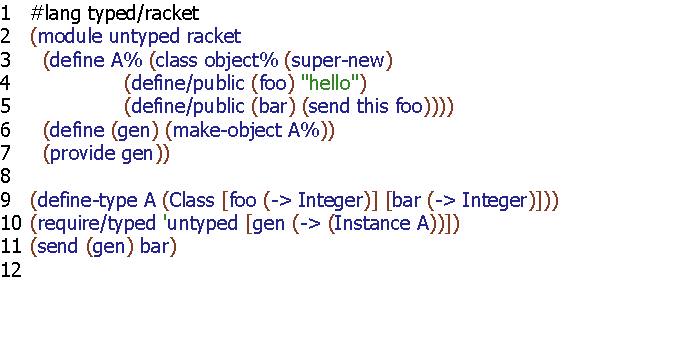
\includegraphics[scale=.7]{../figures/internal.pdf}&\hspace{-2cm}
\begin{minipage}{.5\textwidth}
\vspace{-4.3cm}
\tiny
\begin{lstlisting}[basicstyle=\scriptsize\ttfamily]
foo: broke its own contract
  promised: Integer
  produced: "hello"
  in: the foo method in
      the range of
      (->
       (object/c
        (bar (-> any/c Integer))
        (foo (-> any/c Integer))))
  contract from: (interface for gen)
  contract on: gen
  blaming: (interface for gen)
\end{lstlisting}
\end{minipage}
\end{tabular}
\caption{Typed Racket ensures that internal untyped calls respect external types}
\label{fig:arktex3}
\end{figure}

This issue is illustrated in figure~\ref{fig:intbeh2}, where the source program
initially requires \n to take \xt{A} and return \xt{A}, then requires it to take
and return \xt{B}. If we lift the methods up verbatim (adding only the trivial
casts), then we end up with a type-incorrect wrapper. As a result, we have to
dynamically insert casts inside of the lifted method bodies, ensuring that they
remain type correct in the wrapper class. This operation is depicted in detail
in the appendix.


\begin{figure}[!ht]
\begin{tabular}{l@{\hspace{0.05\textwidth}}l@{\hspace{0.05\textwidth}}l}
\begin{minipage}{0.3\textwidth}
\begin{lstlisting}
class A {n(x:*):*{x}}
class B {m(x:*):*{x}}
class C { 
  m(x:A):A { 
    this.n(x) }
  n(x:A):A { x }}
class D { 
  m(x:A):A { x }
  n(x:B):B { x }}
(<D>new C()).m(
  new C())
\end{lstlisting}
\end{minipage}
&
\begin{minipage}{0.25\textwidth}
\begin{lstlisting}
class DW {
  that : C
  

  m(x:A):A { 
    this.n(x) }

  n(x:B):B { 
    (*@\hspace{-1.5mm}\BehStart\hspace{-1.5mm}@*)B(*@\BehEnd@*)(*@\ShaStart\hspace{-1.5mm}@*)B(*@\ShaEnd\hspace{0mm}@*)
    (*@\hspace{-0.5mm}\BehStart\hspace{-1.5mm}@*)A(*@\BehEnd@*)(*@\ShaStart\hspace{-1.5mm}@*)A(*@\ShaEnd\hspace{0mm}@*)x }
}
\end{lstlisting}
\end{minipage} &
\begin{minipage}{0.3\textwidth}
\begin{lstlisting}
class DW {
  that : C

  m(x:A):A { 
    (*@\hspace{-0.5mm}\BehStart\hspace{-1.5mm}@*)A(*@\BehEnd@*)(*@\ShaStart\hspace{-1.5mm}@*)A(*@\ShaEnd\hspace{0mm}@*)this.n(
      (*@\hspace{-0.5mm}\BehStart\hspace{-1.5mm}@*)B(*@\BehEnd@*)(*@\ShaStart\hspace{-1.5mm}@*)B(*@\ShaEnd\hspace{0mm}@*)x) }

  n(x:B):B { 
    (*@\hspace{-1.5mm}\BehStart\hspace{-1.5mm}@*)B(*@\BehEnd@*)(*@\ShaStart\hspace{-1.5mm}@*)B(*@\ShaEnd\hspace{0mm}@*)
      (*@\hspace{-0.5mm}\BehStart\hspace{-1.5mm}@*)A(*@\BehEnd@*)(*@\ShaStart\hspace{-1.5mm}@*)A(*@\ShaEnd\hspace{0mm}@*)x }
}
\end{lstlisting}
\end{minipage} \\
Source & Type-incorrect & Type-corrected
\end{tabular}
\caption{Wrapper generation}
\label{fig:intbeh2}
\end{figure}

The other major concern when designing a wrapper-based protection system for
objects is that losing methods is a real possibility. If a wrapper zealously
enforces its type, then it will not wrap methods that do not appear on its
type, which can then be lost to later untyped or more-typed code that is
given that wrapper.
Our approach avoids this by inserting ``passthrough'' methods that retain their
original types and behaviors into the output wrappers, as illustrated in
figure~\ref{ctod}, where we make a \C into a \D and then back again. When we
reduce the set of required methods by casting a \C to a \D, we retain the method
\mp by adding it to the output class. Notably, this operation preserves existing
subtyping relationships, as the generated wrappers only appear as values, and
the operation only adds additional methods.

%%%%%%%%%%%%%%%%% EXAMPLE  <C><D>new C %%%%%%%%%%%%%%%%%%%%%%%%%%%%%%%%%%%%
\begin{figure}[h!]
\footnotesize
\begin{tabular}{ll}\begin{minipage}{6cm}
\[\begin{array}{l}
\class ~\C~ \{\\
\SP  \Mdef\m\x\E\E\x\\
\SP  \Mdef\mp\x\E\E\x\\
\}\\[2mm]
\class ~\EMxt{CtoD}~ \{\\
\SP  \Fdef\that\C\\
\SP  \Mdef \m\x\any\any{\BehCast\any{\ShaCast\any{\BehCast\E{\ShaCast\E\x}}}}\\
\SP  \Mdef \mp\x\E\E{\x}\\
\}\\
\end{array}\]
\end{minipage}
&
\begin{minipage}{5cm}
\[\begin{array}{l}
\class ~\D~ \{\\
\SP  \Mdef\m\x\any\any\x\\
\}
\\
\\[2mm]
\class ~\EMxt{CtoDtoC}~ \{\\
\SP  \Fdef\that{\EMxt{CtoD}}\\
\SP  \HT{\m(\HT\x\E)}{\E}\;\{\BehCast\E{\ShaCast\E{\BehCast\any{\ShaCast\any{}}}} \\
\SP ~~~~{\BehCast\E{\ShaCast\E{\BehCast\any{\ShaCast\any\x}}}}\}\\
\SP  \Mdef\mp\x\E\E{ \BehCast\E{\ShaCast\E{\BehCast\E{\ShaCast\E\x}}}}\\
\SP  \Mdef\mp\x\any\any{ \BehCast\any{\Call\this\mp{\BehCast\E{\ShaCast\E{\x}}}}}\\
\}\\
\end{array}\]
\end{minipage}
\end{tabular}
\caption{Wrapper classes generated by \BehCast\C{(\BehCast\D{\New\C{}})}}
\label{ctod}
\end{figure}

The Typed Racket translation demonstrates some of the key issues inherent in
a wrapper-based system, where wrapper-inserting casts build up very quickly
internally, leading to the potential for a wrapper explosion, as previously
noted by Takikawa et al~\cite{practical-gt}, a point that is further
highlighted by the number of casts inserted into the wrappers.




\begin{figure}[!t]
\small
\begin{tabular}{@{}cc}
  \begin{tabular}{|@{}cc@{\hspace{1mm}}|}\hline
  \begin{minipage}{4.6cm}
    \begin{lstlisting}
class A {
 m(x:A):A {this}}

class I {
 n(x:I):I {this}}

class T {
 s(x:I):T {this}
 t(x:*):* {this.s(x)}}
      \end{lstlisting}    
  \end{minipage}
&
  \begin{minipage}{4.6cm}
    \begin{lstlisting}
class A {
 m(x:A): A {this}}

class I {
 m(x:C):I {this}}

class T {
 s(x:I):T {this}
 t(x:*):* {this.s(x)}}
      \end{lstlisting}    
  \end{minipage}
\\[2mm]
(Litmus test 1) & (Litmus test 2)\\[3mm]
  \begin{minipage}{4.3cm}
    \begin{lstlisting}
class A {
 m(x:*):* {this}}

class I {
 m(x:C):C {x}}

class J {
 m(x:D):D {x}}

class E {f:I g:J}

class T {
 t(x:*):* {
   new E(x,x)}}
      \end{lstlisting}    
  \end{minipage}
&
  \begin{minipage}{4.6cm}
    \begin{lstlisting}
class A {
 f:*
 m(x:A):A {
  this.f(new A(new C()))}}


class I {
 f:D
 m(x:I):I {this}}


class T {
 s(x:I):I {x.m(x)}
 t(x:*):* {this.s(x)}}
      \end{lstlisting}    
  \end{minipage}
\\[2mm]
(Litmus test 3) &  (Litmus test 4)\\\hline
  \end{tabular}
  &
\begin{minipage}{4cm}
\begin{tabular}{|@{}c@{\hspace{1mm}}|}\hline
  \begin{minipage}{4cm}
    \begin{lstlisting}
class C { 
  n(x:C):C {this}}

class D {
  o(x:D):D {this}}
    \end{lstlisting}    
  \end{minipage}
 \\
  (Auxiliary classes)\\\hline
\end{tabular}
\\ \\ \\  
\begin{tabular}{|@{}c@{\hspace{1mm}}|}\hline
  \begin{minipage}{4cm}
    \begin{lstlisting}
new T()@t(new A())
    \end{lstlisting}    
  \end{minipage}
  \\
  (Program 1-3)\\\hline
\end{tabular}
\\ \\ \\  
\begin{tabular}{|@{}c@{\hspace{1mm}}|}\hline
  \begin{minipage}{4cm}
    \begin{lstlisting}
new T()@t(
    new A(new D()))
    \end{lstlisting}    
  \end{minipage}
  \\
  (Program 4)\\\hline
\end{tabular}
\end{minipage}
\end{tabular}


\center
\renewcommand{\V}{\EM{\checkmark}}
\begin{tabular}{|r|l@{~}l@{~}l@{~}l|}\hline
                     & L1 & L2 & L3 & L4\\\hline\rowcolor{Gray}
Thorn                &    &    &    &   \\
Typed Racket         &    & \V & \V &  \\\rowcolor{Gray}
Monotonic  RetPy     &    & \V &    &   \\
Transient RetPy      &    & \V & \V & \V \\\rowcolor{Gray}
TypeScript           & \V & \V & \V & \V \\\hline
\end{tabular}  
  \caption{Semantic litmus tests.}\label{litmus}
\end{figure}


\subsection{Trace preservation}

One outcome of our work is showing how \emph{all} of the gradual type systems
are observationally distinct.  \figref{litmus} presents four litmus tests that
are sufficient to distinguish the five type systems being studied in this
paper.  Each litmus test is a program composed of a class table and a main
expression. The programs are written in \kafka syntax but equivalent
programs can be expressed in each of the target languages. All programs are
well-typed in each of the respective type systems and give raise to
different runtime errors. Under TypeScript semantics, all programs run to
completion without getting stuck. With Thorn, all litmus programs fail at a structural cast from \code A to \code I.  For the other languages the situation is
as follows:
\begin{itemize}
\item {\bf L1:} Fails because \code A is not a subtype of \code I, the
  failure is at a shallow cast because \code A does not have all the methods of
  \code I.   \FZ{CHECK, we do not have shallow casts, is this still relevant?}
\item{\bf L2:} Succeeds in Monotonic/Transient/Racket because shallow casts
  of \code A to \code I go through. \FZ{CHECK, we do not have shallow casts, is this still relevant?  Cite monotonic here?}
\item{\bf L3:} Fails in Monotonic because the same object is being cast to
  two different types, \code I and \code J.  \FZ{CHECK, cite monotonic or not?}
\item{\bf L4:} Fails in Monotonic because the object refereed to by \code x
  in method \code s is cast to \code I. This updates the effective type of field
  \code f to \code D. However, the assignment in method \code m tries to give it
  an \code A. This fails in Racket because the \this field is wrapped with an
  \code I type, and the assignment to \code f does not respect that type.
\end{itemize}

\section{Implementation} We designed \kafka to have a close correspondence to
the intermediate languages (ILs) used by common VMs, but by necessity the
correspondence is not exact; real ILs are far too complex to be easily
presented or formally reasoned about. To validate this aspect of \kafka's
design, we implemented a compiler from \kafka to C\#, alongside a runtime that
provides the key behavioral cast operation.

The key challenge that we encountered in the development of this compiler
relates to one of our earliest design choices: the use of a structural type
system. As previously mentioned, structural typing is common in gradually
typed languages, but is very uncommon in actual virtual machines, especially
those that already have static typing like the CLR or the JVM. In order to
implement \kafka by translation to C\#, we have to convert \kafka's structural
types to C\# nominal types, maintaining semantic equivalence.

\subsection{Structural to Nominal Translation} Our implementation of the
conversion of \kafka to C\# types is based on a whole program type analysis.
Consider a (structural) class table \K, and assume that $\StrSub{}\K\t\tp$ for
some $\t$ and $\tp$. C\# already handles the case where $\t$ or $\tp$ is
$\any$, via its \xt{dynamic} type, which has the same semantics, but if $\t$
and $\tp$ are classes $\C$ and $\D$, then we have to be more careful.

The approach works by introducing the interface \xt{ID}, which the translated
version of $\C$ implements. \xt{ID} has all of the same methods as $\D$ did,
allowing the same operations to be performed on its instances. We then refer
to $\D$ by \xt{ID} in the generated C\# type signatures and casts, which then
allows our translation of the class $\C$ to be used wherever a $\D$ is
expected, satisfying subtyping. If we apply this to every pair of types $\C$
and $\D$ where the subtyping relation holds, the C\# subtyping relation
mirrors the \kafka one exactly.

We chose C\# for this translation because it provides the natural
correspondence between our $\any$ and its \xt{dynamic}. However, C\# also
created a substantial problem for our implementation, for it does not allow
for covariance or contravariance in interface implementation, whereas \kafka's
subtyping mechanism does allow both. However, C\# does allow for
\emph{explicit implementations}, which we use to implement covariant and
contravariant interface implementation, by explicitly calling out the
interface method to implement and forwarding to the actual implementation.

\subsection{Validation of \kafka}

The goal of our implementation was to validate the choice of features to
include in \kafka by showing that they are similar to those provided in
modern, high performance VMs, and for most of \kafka's functionality, the
implementation was trivial. However, structural typing proved difficult, both
because of fundamental differences forcing the generation of a very large and
fixed inheritance hierarchy, and because of specific design choices made in
C\#. Even when making a major assumption - the closed-world restriction - our
implementation of structural typing on top of a nominal type system is
relatively non-trivial. While some practical, sound, implementations of
structurally typed languages exist (with Scala being the most notable),
structural typing creates fundamental difficulties in using off-the-shelf VMs.

What our implementation does not do is provide an accurate picture of the
performance of the gradual typing systems in question, rather focusing on
semantic differences. This limitation is due to a wide range of factors,
including having none of the commonly-cited performance optimizations, such as
threesomes~\cite{siek10}, combined with the severe inherent restrictions on
what programs can be reasonably written in \kafka. As a result, any
performance evaluation based on our \kafka implementation would not be
representative of the performance of a real implementation. %\clearpage

\section{Conclusion}

Gradual typing is no longer simply a popular research topic in academia.
Real-world applications are being written with gradual types and the tug of
war between soundness and performance is being played out in multiple
language designs.  It is the responsibility of language researchers to
present a clear understanding of each viable gradual typing idiom available.
We have introduced \kafka, a formal language that serves as the foundation
for deconstructing five existing gradual typing systems: Typescript, Thorn,
Transient Python, and Typed Racket.
%, and Monotonic Python. 
\kafka offers the
opportunity for comparing and contrasting these gradual typing systems
within an unified framework. The translations to \kafka for each gradual
typing system highlights the essences which makes each system unique.


\bibliographystyle{unsrturl}
\bibliography{../../bib/jv,../../bib/all}

\clearpage

\appendix
%%%%%%%%%%%%%%%%%%%%%%%%%%%%%%%%%%%%%%%%%%%%%%%%%%%%%%%%%%%%%%%%%%%%%%%%%%%%%%
%%%%%%%%%%%%%%%%%%%%%%%%%%%%%%%%%%%%%%%%%%%%%%%%%%%%%%%%%%%%%%%%%%%%%%%%%%%%%%
\section{Auxiliary Definitions for \kafka}%%%%%%%%%%%%%%%%%%%%%%%%%%%%%%%%%%%%
%%%%%%%%%%%%%%%%%%%%%%%%%%%%%%%%%%%%%%%%%%%%%%%%%%%%%%%%%%%%%%%%%%%%%%%%%%%%%%
%%%%%%%%%%%%%%%%%%%%%%%%%%%%%%%%%%%%%%%%%%%%%%%%%%%%%%%%%%%%%%%%%%%%%%%%%%%%%%
\label{appendix:kafka}


\subsection{Syntax}

\begin{figure}[!h]
% \hrulefill

\hspace{0.1cm}
\begin{minipage}{5.9cm}\begin{tabular}{@{}l@{~}l@{}l@{}l@{}ll}
\e &::=  \x         &\B \this         &\B \that      \\
   &\B \New\C{\b\e}  &\B \Get\e\f     &\B \Set\e\f\e   \\
   &\B \KCall\e\m\e\t\t &\B \DynCall\e\m\e &\B \SubCast\t\e \\
%    &\B \ShaCast\t\e  
   &\B \a \\
\end{tabular}\end{minipage}
\begin{minipage}{5.9cm}\begin{tabular}{l@{~}l@{}l@{}l}
   ~ \k &::= \Class \C {\b\fd}{\b\md}
%    ~ \k &::= \Class {\C \Exten \Cp} {\b\fd}{\b\md}
\end{tabular}
\begin{tabular}{l@{~}l@{}l@{}l}
% \md &::= \NMdef\m\this\t\x\t\t\e   &\B  \NMdef\f\this\t\x\t\t\e &\B \\ &\qquad \NMdefz\f\this\t\t\e \\
\md &::= \Mdef\m\x\t\t\e   &\B  \Mdef\f\x\t\t\e &\B \Mdefz\f\t\e \\
~ \t&::= ~ \any  \B   \C  \\ 
~\fd&::= ~ \Fdef\f\t \\ 
~\s&::= \{\b{\Bind\a{\obj\C{\b\a}}}\} \\
\end{tabular}\end{minipage}

% \hrulefill
\caption{\kafka Syntax.}
\end{figure}



\subsection{Semantics}

\begin{figure}[!b]
% \hrulefill

\begin{minipage}{8cm}
  \opdef{\Reduce \K\e\s \Kp\ep\sp}
        {\e\s evaluates to \ep\xspace in a step}\\[-1mm]
\begin{tabular}{l@{}l@{~}l@{~}l}
\CondRule{E1}{  %% new C -> a
   \fresh\ap 
}{ 
  \ReduceA \K{\New\C{\b\a}}\s \K\ap{\Map\s{\Bind\ap{\obj\C{\b\a}}}}
}
\CondRule{E2}{  %% a.f() -> e
    \Mdefz\f\t\e \In \App\K\C \AND  \App\s\a =\obj\C{\b\a}
}{
   \ReduceA \K{\Get\a\f}\s \K{[\a/\this]\e}\s
}
\CondRule{E3}{  %% a.f(a) -> e
    \Mdef\f\x\t\t\e \In \App\K\C \AND  \App\s\a=\obj\C{\b\a}
}{
   \ReduceA \K{\Set\a\f\ap}\s \K{[\a/\this~{\ap/\x}]\e}\s
}
\CondRule{E4}{  %% a.f() -> e
 \readf \s\a\f\K =  \ap 
}{
  \ReduceA \K{\Get\a{\f}}\s  \K\ap\s
}
\CondRule{E5}{  %% a.f(e) -> e
 \setf \s\a\f\ap\K =  \sp
}{
  \ReduceA \K{\Set\a{\f}\ap}\s \K\ap\sp
}
\CondRule{E6a}{  %% a.m(a) -> e
  \Mdef\m\x\tp\t\e  \In \App\K\C \AND \App\s\a=\obj\C{\b\a}
}{
 \ReduceA \K{\KCall\a\m\ap\tp\t}\s \K{[\a/\this~{\ap/\x}]\e}\s
}
\CondRule{E7}{  %% a@m(a) -> e
    \Mdef\m\x\any\any\e \In \App\K\C \AND \App\s\a=\obj\C{\b\a}
}{
  \ReduceA \K{\DynCall\a\m\ap}\s \K{[\a/\this~{\ap/\x}]\e}\s
}
\CondRule{E8}{  %% Subtypecast
}{ 
  \ReduceA \K{\SubCast \any\a}\s \K\a\s
}
\CondRule{E9}{  %% Subtypecast
  \StrSub {}\K\C \D \AND \App\s\a=\obj\C{\b\a} 
}{ 
  \ReduceA \K{\SubCast \D\a}\s \K\a\s
}
\CondRule{E10}{  %% E[e] -> E[e']
  \Reduce \K\e\s \Kp\ep\sp
}{
 \ReduceA \K{\EE[\e]}\s \Kp{\EE[\ep]}\sp
}
\end{tabular}\end{minipage}

%%%%%%%%%%%%%%%%%%% CONTEXTS %%%%%%%%%%%%%%%%%%%%%%%%%%%%%%%%%%%%%%%%%%%%
~\\[2mm]

\begin{minipage}{4cm}\begin{tabular}{l@{~~}l@{~}l@{~}l@{~}l@{~}l@{~}l@{~}l}
\EE &::= \Get\EE\f     &\B
        \Set\EE\f\e   &\B
        \Set\a\f\EE   &\B  
        \KCall\EE\m\e\t\t  &\B
        \KCall\a\m{\EE}\t\t &\B
        \DynCall\EE\m\e   &\B
        \DynCall\a\m\EE   \\
   &\B~
       \SubCast\t\EE  &\B
       \New\C{\b \a\,\EE\,\b\e}
  &\B \EM{\square}
\end{tabular}
\end{minipage}

% \hrulefill
\caption{\kafka Semantics.}
\end{figure}

%\clearpage

\subsection{Subtyping}

The structural subtype relation, written \StrSub\M\K\t\tp, asserts that \t
is a subtype of \tp in the environment \M composing a set of subtype relations and
a class table \K.   The set of subtype relations can be omitted if its empty.

~\\

\opdef{\StrSub\M\K\t\tp}{\t is a subtype of \tp}
\begin{mathpar}
\IRule{SRef}{
}{
 \StrSub\M\K \t \t
}

\IRule{SAss}{
\C \Sub \D \in \M
}{
 \StrSub \M\K \C\D
}

\IRule{SRec}{
 \M' = \M~\C\Sub\D\\
\mt \in \classoff\D\K \implies \mtp \in \classoff\C\K ~.~ \StrSub{\M'}\K\mt{\mtp}
}{
 \StrSub \M\K \C \D 
}
\end{mathpar}

\opdef{\StrSub\M\K\mt\mtp}{\mt is a subtype of \mtp}
\begin{mathpar}
\IRule{SMet}{
  \StrSub \M\K {\t[1]} {\t[2]} \\
  \StrSub \M\K {\tp[2]} {\tp[1]}
}{
 \StrSub \M\K {\Mtype\m{\t[1]}{\tp[1]}} {\Mtype\m{\t[2]}{\tp[2]}}
}

\IRule{SGet}{
  \StrSub \M\K {\t[1]} {\t[2]}
}{
 \StrSub \M\K {\Mtype\f{}{\t[1]}} {\Mtype\f{}{\t[2]}}
}

\IRule{SSet}{
  \StrSub \M\K {\t[1]} {\t[2]}
}{
 \StrSub \M\K {\Mtype\f{\t[1]}{\t[1]}} {\Mtype\f{\t[2]}{\t[2]}}
}
\end{mathpar}

\subsection{Well-formedness}

The well-formedness judgments for \kafka are defined for programs, classes, methods, fields, and types.

~\\

\opdef{~\WFq{\K~\e~\s}}{Well-formed program}

\begin{mathpar}
\IRule{WP}{
  \k \in \K \implies \WF{}\cdot\K\k \\
  \EnvType\Env\s\K\e\t \\
  \WFtype\K\s
}{
  \WFq{\K~\e~\s}
}
\end{mathpar}

\opdef{\WF{}\s\K {\Class\C{\b\fd}{\b\md}}}{Well-formed class}

\begin{mathpar}
\IRule{WC}{
 \xt{overloading}_{\emptyset}(\b\md~\b\fd)\OK \\
 \fd\in\b\fd\implies \WF {}{}\K \fd \\
 \md\in\b\md\implies \WF {\text{this}:\C~}\s\K \md 
}{
 \WF {}\s\K {\Class \C {\b\fd}{\b\md}}
}
\end{mathpar}

The \xt{overloading} auxiliary function states that there are no overloaded 
field or method names within the given field and method definitions. \\

\opdef{~\WF \Env\s\K \md}{Well-formed methods}
\begin{mathpar}
\IRule[width=18em]{WT1}{
 \EnvType {\Env{~\Ftype\x\any}~}\s\K\e\any\\
 \WFtype\K\any \\
}{
 \WF \Env\s\K {\Mdef\m\x\any\any\e}
}

\IRule{WS1}{
 \EnvType {\Env{~\Ftype\x\any}~}\s\K \e\any \\
 \WFtype \K\any 
}{
 \WF  \Env\s\K {\Mdef\f\x\any\any\e}
}

\IRule{WG1}{
 \EnvType \Env\s\K\e\any \\
 \WFtype \K\any
}{
 \WF \Env\s\K {\Mdefz\f\any\e}
}
\end{mathpar}

\begin{mathpar}
\IRule[width=18em]{WT2}{
 \EnvType {\Env{~\Ftype\x\C}~}\s\K\e\Cp\\
 \WFtype\K\C \\
 \WFtype\K\Cp \\
}{
 \WF \Env\s\K {\Mdef\m\x\C\Cp\e}
}

\IRule{WS2}{
 \EnvType {\Env{~\Ftype\x\Cp}~}\s\K \e\C \\
 \WFtype \K\C 
}{
 \WF  \Env\s\K {\Mdef\f\x\C\C\e}
}

\IRule{WG2}{
 \EnvType \Env\s\K\e\C \\
 \WFtype \K\C
}{
 \WF \Env\s\K {\Mdefz\f\C\e}
}
\end{mathpar}

\opdef{~\WFtype \K {\fd}}{Well-formed fields}
\begin{mathpar}
\IRule{WF}{
 \WFtype\K\t 
}{
 \WFtype\K{\Fdef\f\t}
}
\end{mathpar}
 
\opdef{~\WFtype\K\t}{Well-formed types}
\begin{mathpar}
\IRule{WA}{
}{
 \WFtype\K\any
}

\IRule{WC}{
 \C \in \K
}{
 \WFtype\K\C
}
\end{mathpar}

\opdef{~\WFtype\K\s}{Well-formed heaps}
\begin{mathpar}
\IRule{WH}{
\Bind\ap{\obj\C{\a_1 \ldots \a_n}}~\in~\s \implies \Class\C{\HT{\f_1}{\t_1} \ldots \HT{\f_n}{\t_n}}{\b\md}\in\K~\wedge \\ 
\EnvType\cdot\s\K{\a_1}{\t_1} ~\ldots~ \EnvType\cdot\s\K{\a_n}{\t_n}
}{
 \WFtype\K\s
}
\end{mathpar}

\subsection{Expression typing}

The expression typing judgments for \kafka includes in ascending order as listed in the formalism:
variable, untyped address, subsumption, field set, field get, static method invocation, dynamic method invocation, object creation,
subtype cast,
% shallow cast, 
typed address, \xt{that} field get, and \xt{that} field set.

Field access rules W3 and W4 require a typed receiver, since \any does not
have any methods a receiver typed at \any will never typecheck.

Shallow casts, W9, do not change the type of the expression, as we are casting
to the name of \t not to \t.  

~\\

\opdef{\EnvType\Env\s\K\e\t}{\e has type \t in environment \Env against heap \s and class table \K}
\begin{mathpar}

\IRule{W1}{
   \HasType \Env\x\t
 }{
   \EnvType \Env\s\K\x\t
}

\IRule{W2}{ 
  \EnvType \Env\s\K\e\tp \\
 \StrSub \cdot\K \tp \t
 }{
  \EnvType \Env\s\K\e\t 
}   

\IRule{W3}{
  \EnvType \Env\s\K\e\C \\
  \Mtype \f{}\t \in \classoff\C\K
}{
  \EnvType \Env\s\K{\Get\e\f}\t
}    

\IRule[width=20em]{W4}{
  \EnvType \Env\s\K\e\C \\
  \Mtype \f\t\t \in \classoff\C\K  \\
  \EnvType \Env\s\K\ep\t
}{
  \EnvType \Env\s\K{\Set\e\f\ep}\t
}    

\IRule[width=20em]{W5}{
  \EnvType \Env\s\K\e\C \\
  \Mtype \m\t\tp\in \classoff\C\K  \\
  \EnvType \Env\s\K\ep\t
}{
  \EnvType \Env\s\K{\KCall\e\m\ep\t\tp}\tp
}    

\IRule{W6}{
  \EnvType \Env\s\K\e\any \\
  \EnvType \Env\s\K\ep\any
}{
  \EnvType \Env\s\K{\DynCall\e\m\ep}\any
}    

\IRule{W7}{
 \EnvType \Env\s\K{\e_1}{\t_1}\dots 
 \EnvType \Env\s\K{\e_n}{\t_n}\ \\ 
 \b\fd=\Fdef{\f_1}{\t_1}\dots\Fdef{\f_n}{\t_n} \\ 
  \Class \C {\b\fd}{\b\md} \in \K
}{
  \EnvType\Env\s\K{\New\C{\e_1\dots\e_n}}\C
}

\IRule{W8}{
  \EnvType \Env\s\K\e\tp
}{
  \EnvType \Env\s\K{\SubCast\t\e}\t
}

\IRule{W9}{
  \s(\a) = \obj\C{\b\ap}
}{
  \EnvType \Env\s\K\a\C
}

\IRule{W10}{
 }{
   \EnvType \Env\s\K\a\any
}
\end{mathpar}


\subsection{Field read}

The function $\readf\s\a\f\K$ reads the value in the field \f in the object \a.

\begin{equation*}
\readf \s\a\f\K = \ap 
  ~~\mathit{if}~~ \begin{cases}  \s(\a) = \obj\C{\a_1\dots\a_n \ap \dots}\\
 \Class\C {\Fdef{\f_1}{\t_1}\dots\Fdef{\f_n}{\t_n}\Ftype\f\t\dots}{\b\md}\in\K
 \end{cases}
\end{equation*}

\subsection{Field write}

The function \setf\s\a\f\ap\K denotes writing of value \ap to the field \f of
the object stored at \a in \s.

\begin{equation*}
\setf \s\a\f\ap\K= \Map\s{\Bind{\a}{\obj\C{\a_1\dots\a_n\,\ap\dots}}}
  ~~\mathit{if}~~ \begin{cases}
   \s(\a) = \obj\C{\a_1\dots\a_n\,\app\dots}\\
   \Class\C{\Fdef{\f_1}{\t_1}\dots\Fdef{\f_n}{\t_n}\,\Fdef\f\t\dots}{\b\md}\in\K
\end{cases}
\end{equation*}

\subsection{Method overloading}

The function $\xt{overloading}(\b\md ~ \b\fd)$ there are no overloaded method names in the
given method definitions.


\opdef{~\xt{overloading}$_{\cmdp}$(\b\md ~\b\fd)}{Method overloading}
\begin{mathpar}
\IRule{MO1}{
}{
\xt{overloading}_{\cmd}(\emptyset)
}

\IRule{MO2}{
 \Mtype\m\any\any \notin \cmd \\
 \cmdp = \cmd, \Mtype\m\any\any \\
 \xt{overloading}_{\cmdp}(\b\md\,\b\fd)
}{
\xt{overloading}_{\cmd}(\Mdef\m\x\any\any\e~\b\md~\b\fd)
}

\IRule{MO3}{
 \Mtype\m\t\t \in \cmd \implies \t = \any \\
 \cmdp = \cmd, \Mtype\m\t\t \\
 \xt{overloading}_{\cmdp}(\b\md\,\b\fd)
}{
\xt{overloading}_{\cmd}(\Mdef\m\x\C\C\e~\b\md~\b\fd)
}

\IRule{MO4}{
 \f \in \xt{names}(\cmd) \implies \f \notin \xt{names}(\cmd \setminus \Mtype\f{}\t)  \\
 \cmdp = \cmd, \Mtype\f\t\t  \\
 \xt{overloading}_{\cmdp}(\b\md\,\b\fd)
}{
\xt{overloading}_{\cmd}(\Mdef\f\x\t\t\e ~ \b\md ~\b\fd)
}

\IRule{MO5}{
 \f \in \xt{names}(\cmd) \implies \f \notin \xt{names}(\cmd \setminus \Mtype\f\t\t)  \\ \cmdp = \cmd, \Mtype\f\t\t \\
 \xt{overloading}_{\cmdp}(\b\md\,\b\fd)
}{
\xt{overloading}_{\cmd}(\Mdefz\f\t\e ~ \b\md ~ \b\fd)
}
\end{mathpar}

\opdef{~\xt{overloading}(\b\fd)}{field overloading}
\begin{mathpar}
\IRule{FO1}{
 \f \notin \xt{names}(\cmd) \\
 \cmdp = \cmd, \Fdef\f\t \\
 \xt{overloading}_{\cmdp}(\b\fd)
}{
\xt{overloading}_{\cmd}(\Fdef\f\t ~ \b\fd)
}
\end{mathpar}

% \subsection{Source Method Overloading}
% 
% \opdef{~${\soverloading_{\cmdp}(\b\md ~\b\fd)}$}{Method overloading}
% \begin{mathpar}
% \IRule{MSO1}{
% }{
% {\soverloading_{\cmd}(\emptyset)}
% }
% 
% \IRule{MSO2}{
%  {\Mtype\m\t\t \notin \cmd} \\
%  {\cmdp = \cmd, \Mtype\m\t\t} \\
%  {\soverloading_{\cmdp}(\b\md)}
% }{
%  {\soverloading_{\cmd}(\Mdef\m\x\t\t\e~\b\md~\b\fd)}
% }
% \end{mathpar}
% 
% \opdef{~${\soverloading(\b\fd)}$}{field overloading}
% \begin{mathpar}
% \IRule{FSO1}{
%  {\f \notin \xt{names}(\cmd)} \\
%  {\cmdp = \cmd, \Fdef\f\t} \\
%  {\soverloading_{\cmdp}(\b\fd)}
% }{
% {\soverloading_{\cmd}(\Fdef\f\t ~ \b\fd)}
% }
% \end{mathpar}

\section{Complete translation for TypeScript}

\subsection{TypeScript translation for program, class, and method}

\opdef{$\progtrans {\e~\K}{\e'~{\K'}}$}{TypeScript translation for programs}
\opdef{$\classtrans {\K} {\Class \C{...}{...}~\K} {\Class \C{...}{...}~\K}$}{TypeScript translation for classes} 
\opdef{$\methtrans {\K}{\C}{\md}{\md'}{}$}{TypeScript translation for methods} 
\opdef{$\fieldtrans {\fd}{\fd'}{}$}{TypeScript translation for fields} 

\begin{mathpar}
\IRule[width=20em]{TS-PROGRAM}{
  {\classtrans{\K}{\K}{\K'}} \\ \GenCast{\K}{\cdot}{\e}{\ep}{\t} 
}{\progtrans{\e~\K}{\e'~{\K'}}}

\IRule[width=30em]{TS-CLASS1}{ 
  \cload{\b\md ~ \b\fd}\\
  \b{\methtrans {\K}{\C}{\md}{\md'}{}} \\
  \b{\fieldtrans {\fd}{\fd'}{}} \\
  {\C \not\in \Kp} \\
  \classtrans {\K}{\Kp}\Kpp
}{
   \classtrans {\K}{{\Class \C{\b{\fd}}{\b\md}~\Kp}}{\Class \C {\b{\fd'}}{\b{\md'}}~\Kpp}}

\IRule{TS-CLASS2}{ 
}{
  \classtrans {\K}\cdot\cdot
}

\IRule{TS-FIELD}{
}{
  \fieldtrans{\Fdef\f\t}{\Fdef\f\any}{}
}

\IRule{TS-METHOD}{
  \AnaCast {\K}{\HT\this{\C}~\HT\x{\t}}{\e}\ep{\tp}
}{
  \methtrans {\K}{\C}{\Mdef\m\x{\t}{\tp}{\e}}{\Mdef\m\x\any\any{\SubCast\any\ep}}{}
}
\end{mathpar}

\subsection{TypeScript synthetic translation for expressions}

\opdef{$\GenCast\K\Env{\e}{\ep}{\t}$}{$\e$ translates to $\ep$ producing type $\t$, with context $\Env$ and class table $\K$}

% \begin{mathpar}

\colorbox[gray]{1}{
\begin{minipage}{\textwidth}
\begin{mathpar}
\IRule{TSS-VAR}{\HasType{\Env}\x\t}{\GenCast{\K}\Env\x\x\t}

\IRule[width=30em]{TSS-TYCALL}{
    \GenCast\K\Env{\e_1}{\e_3}{\C} \\ \m({\t_1}):\t_2 \in \classoff\C\K \\ {\AnaCast\K\Env{\e_2}{\e_4}{\t_1}}
}{
    \GenCast\K\Env{\Call{\e_1}\m{{\e_2}}}{\DynCall{\SubCast\any{\e_3}}\m{\SubCast\any{\e_4}}}{\t_2}
}

\IRule[width=10em]{TSS-DYCALL}{
    \GenCast\K\Env{\e_1}{\e_3}{\any} \\ {\AnaCast\K\Env{\e_2}{\e_4}{\any}}
}{
    \GenCast\K\Env{\Call{\e_1}\m{{\e_2}}}{\DynCall{\e_3}\m{{\e_4}}}{\any}
}

\IRule[width=20em]{TSS-FIELD}{
    {\HasType{\Env}\this\C} \\ 
    {\f(\b{\t}):\t \in \classoff\C\K} \\ 
    \b{\AnaCast\K\Env{\e}{\ep}{\t}}
}{
    \GenCast\K\Env{\Call{\this}\f{\b\e}}{\Call{\this}\f{\b\ep}}{\t}
}

\IRule{TSS-NEW}{
  \b{\AnaCast{\K}\Env{\e_1}{\e_2}\t} \\ 
  {\Class \C {\b{\Fdef\f\t}} {\b{\md}} \in \K}
}{
  \GenCast\K\Env{\New\C{\b{\e_1}}}{\SubCast\any{\New\C{\b{\e_2}}}}{\C}
}
\end{mathpar}
\end{minipage}
}


\subsection{TypeScript analytic translation for expressions}

\opdef{$\AnaCast\K\Env\e\ep\t$}{$\e$ translates to $\ep$ against type $\t$, with context $\Env$ and class table $\K$}

\colorbox[gray]{1}{
\begin{minipage}{\textwidth}
\begin{mathpar}
\IRule{TSA-SUB}{
  \GenCast\K\Env\e\ep\tp \\
  {\K \vdash \tp \Sub \t}
}{
  \AnaCast\K\Env\e\ep\t
}

\IRule{TSA-TRANS1}{
  \GenCast\K\Env\e\ep\any
}{
  \AnaCast\K\Env\e\ep\t
}

\IRule{TSA-TRANS2}{
  \GenCast\K\Env\e\ep\C
}{
  \AnaCast\K\Env\e\ep\any
}
\end{mathpar}
\end{minipage}
}


\section{Complete translation for Thorn}

\subsection{Thorn Type Translation}
\opdef{$\Kt{\t} = \src{\tp}$}{The \kafka equivalent of $\t$ is $\tp$}

\begin{mathpar}
\IRule{THT-ANY}{
}{
  \src\any = \Kt{\any}
}

\IRule{THT-CONC}{
}{
  \src\C = \Kt{\C}
}

\IRule{THT-WEAK}{
}{
  \src\any = \Kt{\dt\C}
}
\end{mathpar}
\opdef{$\progtrans {\e~\K}{\e'~{\K'}}$}{Thorn translation for programs}
\opdef{$\classtrans {\K} {\Class \C{...}{...}~\K} {\Class \C{...}{...}~\K}$}{Thorn translation for classes} 
\opdef{$\methtrans {\K}{\C}{\md}{\md'}{}$}{Thorn translation for methods} 
\opdef{$\fieldtrans {\fd}{\fd'}{}$}{Thorn translation for fields} 
\begin{mathpar}
\IRule[width=20em]{TH-PROGRAM}{
  {\classtrans{\K}{\K}{\K'}} \\ \GenCast{\K}{\cdot}{\e}{\ep}{\t} 
}{\progtrans{\e~\K}{\e'~{\K'}}}

\IRule[width=30em]{TH-CLASS1}{ 
  \cload{\b\md ~ \b\fd}\\
  \b{\methtrans {\K}{\C}{\md}{\md'}{}} \\
  \b{\fieldtrans {\fd}{\fd'}{}} \\
  {\C \not\in \Kp} \\
  \classtrans {\K}{\Kp}\Kpp
}{
   \classtrans {\K}{{\Class \C{\b{\fd}}{\b\md}~\Kp}}{\Class \C {\b{\fd'}}{\b{\md'}}~\Kpp}}

\IRule{TH-CLASS2}{ 
}{
  \classtrans {\K}\cdot\cdot
}

\IRule{TH-FIELD}{
  \src\tp = \Kt\t
}{
  \fieldtrans{\Fdef\f\t}{\Fdef\f\tp}{}
}

\IRule[width=25em]{TH-METHODANY}{
  \AnaCast {\K}{\HT\this{\C}~\HT\x{\t[1]}}{\e}\ep{\t[2]} \\
  \src{\Kt{\t[1]} = \Kt{\t[2]} = \any}
}{
  \methtrans {\K}{\C}{\Mdef\m\x{\t[1]}{\t[2]}{\e}}{\Mdef\m\x{\any}{\any}{\ep}}{}
}

\IRule[width=25em]{TH-METHOD}{
  \AnaCast {\K}{\HT\this{\C}~\HT\x{\Cp}}{\e}\ep{\Cpp} \\
}{
  \methtrans {\K}{\C}{\Mdef\m\x{\Cp}{\Cpp}{\e}}{\begin{array}{c}
    \Mdef\m\x{\Cp}{\Cpp}{\ep} \\
    \Mdef\m\x{\any}{\any}{\SubCast\any{\KCall\this\m{\SubCast\Cp\x}\Cp\Cpp}} \\
  \end{array}}{}
}
\end{mathpar}

\subsection{Thorn synthetic translation for expressions}

\opdef{$\GenCast\K\Env\e\ep\t$}{$\e$ translates to $\ep$ producing type $\t$, with context $\Env$ and class table $\K$}

\begin{mathpar}
\IRule{THS-VAR}{
  \HasType\Env\x\t
}{
  \GenCast\K\Env\x\x\t
}

\IRule[width=30em]{THS-FIELD}{
    \GenCast\K\Env{\e_1}{\e_3}\C \\ 
    {\f(\b{\t_1}):\t_2 \in \classoff\C\K} \\ 
    \b{\AnaCast\K\Env{\e_2}{\e_4}{\t_1}}
}{
    \GenCast\K\Env{\Call{\e_1}\f{\b{\e_2}}}{\Call{\e_3}\f{\b{\e_4}}}{\t_2}
}

\IRule[width=30em]{THS-OPTTCALL}{
    \GenCast\K\Env{\e_1}{\e_3}{\dt\C} \\ 
    {\m({\D_1}):\D_2 \in \classoff\C\K} \\ 
    \AnaCast\K\Env{\e_2}{\e_4}{\D_1}
}{
    \GenCast\K\Env{\Call{\e_1}\m{{\e_2}}}{\SubCast{\D_2}{\DynCall{\e_3}\m{\SubCast\any{\e_4}}}}{\D_2} %Q: do I need to cast the return value of non-bang
}

\IRule[width=20em]{THS-OPTUCALL}{
    \GenCast\K\Env{\e_1}{\e_3}{\dt\C} \\ 
    {\m({\t_1}):\t \in \classoff\C\K} \\ 
    \src{\any} = \Kt{\t[1]}\\
    \AnaCast\K\Env{\e_2}{\e_4}{\t_1} 
}{
    \GenCast\K\Env{\Call{\e_1}\m{{\e_2}}}{\DynCall{\e_3}\m{{\e_4}}}{\t}
    %Q: do I need to cast the return value of non-bang
}

\IRule[width=30em]{THS-TYCALL}{
  \GenCast\K\Env{\e_1}{\e_3}{\D} \\
  {\Mtype\m\t\tp \in \classoff\D\K} \\
  \AnaCast\K\Env{\e_2}{\e_4}{\t}
}{
  \GenCast\K\Env{\Call{\e_1}\m{\e_2}}{\KCall{\e_3}\m{\e_4}\t\tp}{\tp}
}

\IRule{THS-DYCALL}{
    \GenCast\K\Env{\e_1}{\e_3}\any \\ 
    \AnaCast\K\Env{\e_2}{\e_4}\any
}{
    \GenCast\K\Env{\Call{\e_1}\m{{\e_2}}}{\DynCall{\e_3}\m{{\e_4}}}\any
}

\IRule{THS-NEW}{
  \b{\AnaCast\K\Env{\e_1}{\e_2}\t} \\ 
  \Class \C {\b{\Ftype\f\t}} {\b\md} \in \K
  }{
  \GenCast\K\Env{\New\C{\b{\e_1}}}{\New\C{\b{\e_2}}}\C
}
\end{mathpar}
\subsection{Thorn analytic translation for expressions}

\opdef{$\AnaCast\K\Env{\e}{\ep}{\t}$}{$\e$ translates to $\ep$ against type $\t$, with context $\Env$ and class table $\K$}

\begin{mathpar}
\IRule{THA-CSUB}{
  \GenCast\K\Env{\e_1}{\e_2}{\t_2} \\
  {\ThorSub\K\cdot{\t_2}{\t_1}}\\
}{
  \AnaCast\K\Env{\e_1}{\e_2}{\t_1}
}

\IRule{THA-OPTCONC}{
  \GenCast\K\Env{\e_1}{\e_2}{\dt\D} \\ 
  {\ThorSub\K\cdot\D\C}
}{
  \AnaCast\K\Env{\e_1}{\SubCast{\C}{\e_2}}{\C}
}

\IRule{THA-ANYOPT}{
  \GenCast\K\Env{\e_1}{\e_2}{\any} \\
}{
  \AnaCast\K\Env{\e_1}{\e_2}{\dt\C}
}

\IRule{THA-ANYCONC}{
  \GenCast\K\Env{\e_1}{\e_2}{\any} \\
}{
  \AnaCast\K\Env{\e_1}{\SubCast\C{\e_2}}{\C}
}

\IRule{THA-TOANY}{
  \GenCast\K\Env{\e_1}{\e_2}{\t} \\ \t \neq \any
}{
  \AnaCast\K\Env{\e_1}{\e_2}{\any}
}
\end{mathpar}

\subsection{Supporting Text for Thorn}

\subsubsection{Attempted Explanation of Bidirectional}


Cast insertion in our system is illustrated by the following example:

\begin{verbatim}
class C {
  f : C
  m(x:*):* {
    new C(x)
  }
}
\end{verbatim}

Here, in method \m, the only type that \x can possibly have is \any, in spite of the surrounding invocation requiring that it 
be an instance of a \C. Likewise, the only type that makes sense for \New\C\x is \C, despite the return type being declared as
\any. We have to insert casts to make these two cases be well typed, giving us the following translated code:

\begin{verbatim}
class C {
  f : C
  m(x:*):* {
    <*>new C(<C>x)
  }
}
\end{verbatim}

Our cast insertion system is based on this intuition, finding the places where an expression's type is absolute (like \x being 
of type \any), yet is surrounded by an expression that requires it to be something quite different (e.g. \New\C\x requires that
\x must be a \C), drawing on a commonly used approach from type inference, bidirectional typing.

In our approach, we compute ``real'' types using the so-called \emph{synthetic} case of typing, written $\GenCast\K\Env\e\ep\t$,
meaning that $\e$ will always have type $\t$, while translating to $\ep$. Likewise, we enforce ``required'' types through the 
\emph{analytic} judgment, written $\AnaCast\K\Env\e\ep\t$, meaning that if $\e$ is required to be of type $\t$, then the translated
$\ep$ will be of type $\t$.

As a illustrative example, consider $\x$ in the above. We know that $\x$ will always have type $\any$ - expressed as
$\GenCast\K\Env\x\x\any$ by rule \RuleRef{THS-VAR} - no matter what happens around it. However, we also know that $\New\C\x$ 
requires that $\x$ has type $\C$ - expressed as $\AnaCast\K\Env\x?\C$, using ? as a placeholder for the result of translation
- and need to insert a cast so that the types make sense. We can then apply rule \RuleRef{THA-ANYCONC} to \x with \C to find out
that we can make \x have type \C via casting, concluding that $\AnaCast\K\Env\x{\SubCast\C\x}\C$.


\subsubsection{Explanation of Synthetic Cases}
\begin{itemize}
  \item \RuleRef{THS-VAR} is used to determine the type of variables, reporting the variable's type in the context.
  \item \RuleRef{THS-FIELD} determines the type of both field access and assignment, denoted by the field accessors having 0 or 1 arguments, respectively. A field reference will have type $\t$ if the field is of type $\t$, and for a field assignment, the new value must also be of type $\t$.
  \item \RuleRef{THS-OPTTCALL} handles the case when we are making a call 
\end{itemize}

\section{Complete translation for Transient}

\opdef{$\progtrans {\e~\K}{\e'~{\K'}}$}{Transient translation for programs}
\opdef{$\classtrans {\K} {\Class \C{...}{...}~\K} {\Class \C{...}{...}~\K}$}{Transient translation for classes} 
\opdef{$\methtrans {\K}{\C}{\md}{\md'}{}$}{Transient translation for methods} 
\opdef{$\fieldtrans {\fd}{\fd'}{}$}{Transient translation for fields} 
\begin{mathpar}
\IRule[width=20em]{TA-PROGRAM}{
  {\classtrans{\K}{\K}{\K'}} \\ \GenCast{\K}{\cdot}{\e}{\ep}{\t} 
}{\progtrans{\e~\K}{\e'~{\K'}}}

\IRule[width=30em]{TA-CLASS1}{ 
  \cload{\b\md ~ \b\fd}\\
  \b{\methtrans {\K}{\C}{\md}{\md'}{}} \\
  \b{\fieldtrans {\fd}{\fd'}{}} \\
  {\C \not\in \Kp} \\
  \classtrans {\K}{\Kp}\Kpp
}{
   \classtrans {\K}{{\Class \C{\b{\fd}}{\b\md}~\Kp}}{\Class \C {\b{\fd'}}{\b{\md'}}~\Kpp}}

\IRule{TA-CLASS2}{ 
}{
  \classtrans {\K}\cdot\cdot
}

\IRule{TA-FIELD}{
}{
  \fieldtrans{\Fdef\f\t}{\Fdef\f\t}{}
}

\IRule[width=25em]{TA-METHODANY}{
  \AnaCast {\K}{\HT\this{\C}~\HT\x{\any}}{\e}\ep{\any} \\
}{
  \methtrans {\K}{\C}{\Mdef\m\x{\any}{\any}{\e}}{\Mdef\m\x{\any}{\any}{\ep}}{}
}

\IRule[width=25em]{TA-METHOD}{
  \AnaCast {\K}{\HT\this{\C}~\HT\x{\Cp}}{\e}\ep{\Cpp} \\
}{
  \methtrans {\K}{\C}{\Mdef\m\x{\Cp}{\Cpp}{\e}}{
    \Mdef\m\x\any\any{\SubCast\Cp\x ; \ep}}{} % sequencing is sugar
}
\end{mathpar}

\subsection{Transient synthetic translation for expressions}

\opdef{$\GenCast\K\Env{\e}{\ep}{\t}$}{Transient translation for expressions}

\begin{mathpar}
\IRule{TAS-VAR}{\HasType{\E}\x\t}{\GenCast{\K}\E\x{\SubCast\t\x}\t}


\IRule[width=30em]{TAS-TYCALL}{
    \GenCast\K\Env{\e_1}{\e_3}{\C} \\ \m({\t_1}):\t_2 \in \classoff\C\K \\ \b{\AnaCast\K\Env{\e_2}{\e_4}{\t_1}}
}{
    \GenCast\K\Env{\Call{\e_1}\m{{\e_2}}}{\SubCast{\t_2}{\KCall{{\e_3}}\m{\SubCast{\any}{\e_4}}\any\any}}{\t_2}
}

\IRule{TAS-DYCALL}{
    \GenCast\K\Env{\e_1}{\e_3}{\any} \\ {\AnaCast\K\Env{\e_2}{\e_4}{\any}}
}{
    \GenCast\K\Env{\Call{\e_1}\m{{\e_2}}}{\DynCall{\e_3}\m{{\e_4}}}{\any}
}

\IRule[width=20em]{TAS-FIELD}{
    \HasType{\E}\this\C \\ 
    \f(\b{\t_1}):\t_2 \in \classoff\C\K \\ 
    \b{\AnaCast\K\Env{\e_1}{\e_2}{\t_1}}
}{
    \GenCast\K\Env{\Call{\this}\f{\b{\e_1}}}{\Call{\this}\f{\b{\e_2}}}{\any}
}

\IRule{TAS-NEW}{
  \b{\AnaCast{\K}\E{\e_1}{\e_2}\t} \\ 
  \Class \C {\b{\Ftype\f\t}} {\b{\md}} \in \K
  }{\GenCast\K\Env{\New\C{\b{\e_1}}}{\New\C{\b{\e_2}}}{\C}}
\end{mathpar}

\subsection{Transient analytic translation for expressions}

\opdef{$\AnaCast\K\E\e\ep\t$}{Transient translation for bidirectional expressions}

\begin{mathpar}
\IRule{TAA-SUB}{
  \GenCast\K\E\e\ep\tp \\
  \K \vdash \tp \Sub \t
}{
  \AnaCast\K\E\e\ep\t
}

\IRule{TAA-CONS}{
  \GenCast\K\E\e\ep\tp \\
  \consistent\K\tp\t
}{
  \AnaCast\K\E\e{\SubCast\t\ep}\t
}
\end{mathpar}

\section{Complete translation for Typed Racket}

\subsection{Typed Racket translation for program, class, and method}


\opdef{$\progtrans {\e~\K}{\e'~{\K'}}$}{Typed Racket translation for programs}
\opdef{$\classtrans {\K} {\Class \C{...}{...}~\K} {\Class \C{...}{...}~\K}$}{Typed Racket translation for classes} 
\opdef{$\methtranst {\K}{\C}{\md}{\md'}{}$}{Typed Racket translation for typed methods} 
\opdef{$\methtransu {\K}{\C}{\md}{\md'}{}$}{Typed Racket translation for untyped methods} 
\opdef{$\fieldtranst {\fd}{\fd'}{}$}{Typed Racket translation for typed fields} 
\opdef{$\fieldtransu {\fd}{\fd'}{}$}{Typed Racket translation for untyped fields} 
\begin{mathpar}
\IRule[width=20em]{TR-PROGRAM}{
  {\classtrans{\K}{\K}{\K'}} \\ \GenCast{\K}{\cdot}{\e}{\ep}{\t} 
}{\progtrans{\e~\K}{\e'~{\K'}}}

\IRule[width=30em]{TR-TCLASS}{ 
  \cload{\b\md ~ \b\fd}\\
  \b{\methtranst {\K}{\C}{\md}{\md'}{}} \\
  \b{\fieldtranst {\fd}{\fd'}{}} \\
  {\C \not\in \Kp} \\
  \classtrans {\K}{\Kp}\Kpp
}{
   \classtrans {\K}{{\Class \C{\b{\fd}}{\b\md}~\Kp}}{\Class \C {\b{\fd'}}{\b{\md'}}~\Kpp}}

\IRule[width=25em]{TR-UCLASS}{ 
  \cload{\b\md ~ \b\fd}\\
  \b{\methtransu {\K}{\C}{\md}{\md'}{}} \\
  \b{\fieldtransu {\fd}{\fd'}{}} \\
  {\C \not\in \Kp} \\
  \classtrans {\K}{\Kp}\Kpp
}{
   \classtrans {\K}{{\Class \C{\b{\fd}}{\b\md}~\Kp}}{\Class \C {\b{\fd'}}{\b{\md'}}~\Kpp}}

\IRule{TR-CLASS2}{ 
}{
  \classtrans {\K}\cdot\cdot
}

\IRule{TR-TFIELD}{
}{
  \fieldtranst{\Fdef\f\C}{\Fdef\f\C}{}
}

\IRule{TR-UFIELD}{
}{
  \fieldtransu{\Fdef\f\any}{\Fdef\f\any}{}
}

\IRule[width=25em]{TR-TMETHOD}{
  \AnaCast {\K}{\HT\this{\C}~\HT\x{\Cp}}{\e}\ep{\Cpp} \\
}{
  \methtranst {\K}{\C}{\Mdef\m\x{\Cp}{\Cpp}{\e}}{
    \Mdef\m\x\Cp\Cpp{\e} }{}
}

\IRule[width=25em]{TR-UMETHOD}{
  \AnaCast {\K}{\HT\this{\any}~\HT\x{\any}}{\e}\ep{\any} \\
}{
  \methtransu {\K}{\C}{\Mdef\m\x{\any}{\any}{\e}}{
    \Mdef\m\x\any\any{\e} }{}
}
\end{mathpar}

\subsection{Typed Racket synthetic translation}

\opdef{$\GenCast{\K}\Env\e\ep\t$}{Typed Racket synthetic translation}

\begin{mathpar}
\IRule{TRS-VAR}{\HasType{\Env}\x\t}{\GenCast{\K}\Env\x\x\t}

\IRule[width=30em]{TRS-FIELD}{
    \GenCast\K\Env{\e_1}{\e_3}{\C} \\ \f(\b{\t_1}):\t_2 \in \classoff\C\K \\ \b{\AnaCast\K\Env{\e_2}{\e_4}{\t_1}}
}{
    \GenCast\K\Env{\Call{\e_1}\f{\b{\e_2}}}{\Call{\e_3}\f{\b{\e_4}}}{\t_2}
}

\IRule[width=30em]{TRS-TYCALL}{
    \GenCast\K\Env{\e_1}{\e_3}{\C} \\ \m(\Cp):\Cpp \in \classoff\C\K \\ \b{\AnaCast\K\Env{\e_2}{\e_4}{\Cp}}
}{
    \GenCast\K\Env{\Call{\e_1}\m{{\e_2}}}{\KCall{\e_3}\m{{\e_4}}\Cp\Cpp}{\Cpp}
}

\IRule{TRS-DYCALL}{
    \GenCast\K\Env{\e_1}{\e_3}{\any} \\ {\AnaCast\K\Env{\e_2}{\e_4}{\any}}
}{
    \GenCast\K\Env{\Call{\e_1}\m{{\e_2}}}{\DynCall{\e_3}\m{{\e_4}}}{\any}
}

\IRule{TRS-NEW}{
  \b{\AnaCast{\K}\Env{\e_1}{\e_2}\t} \\ 
  \Class \C {\b{\Ftype\f\t}} {\b{\md}} \in \K
  }{\GenCast\K\Env{\New\C{\b{\e_1}}}{\New\C{\b{\e_2}}}{\C}}
\end{mathpar}

\subsection{Typed Racket analytic translation}

\opdef{$\AnaCast\K\Env\e\ep\t$}{Typed Racket analytic translation}

\begin{mathpar}
\IRule{TRA-SUB}{
  \GenCast\K\Env\e\ep\tp \\
  \K \vdash \tp \Sub \t
}{
  \AnaCast\K\Env\e\ep\t
}

\IRule{TRA-WRAP}{
  \GenCast\K\Env\e\ep\tp \\
  \t \neq \tp
}{
  \AnaCast\K\Env\e{\BehCast\t{\ep}}\t
}
\end{mathpar}

\section{Generative Behavioural Casts}

\subsection{Behavioural cast static and dynamic rules}

\begin{minipage}{0.35\textwidth}
\begin{mathpar}
\IRule{WB}{
  \EnvType \Env\s\K\e\tp
}{
  \EnvType \Env\s\K{\BehCast\t\e}\t
}
\end{mathpar}
\end{minipage}
\begin{minipage}{0.5\textwidth}
\begin{tabular}{l@{}l@{~}l@{~}l}
\CondRule{E11}{  %% Behavioral cast  
  \behcast \a\t\s\K  \Kp\ap\sp    
}{    
  \ReduceA  \K{\BehCast \t\a}\s \Kp\ap\sp   
} \\
\multicolumn{4}{l}{\EE ::= \ldots \B \BehCast\t\EE }
\end{tabular}
\end{minipage}

\begin{figure}[!ht]
\vspace{-2mm}

{  
  \begin{mathpar}
  
\IRule{BC1}{
  \App\s\a = \obj\C{\b{\a_1}}  \\
  \fresh\D \\
  \fresh\ap \\
  \cload{\classoff\C\K} \\
  \names{\classoff\Cp\K} \subseteq \names{\classoff\C\K} \\
  \k = \wrap\C{\classoff\C\K}{\classoff\Cp\K}\D \\
  \sp = \Map \s{\Bind\ap{\obj\D{\a}}} \\  
}{
  \behcast\a\Cp\s\K {\K\,\k}\ap\sp
}

\IRule{BC2}{
  \App\s\a = \obj\C{\b{\a_1}}  \\
  \fresh\D \\
  \fresh\ap \\
  \k = \wrapAny\C{\classoff\C\K}\D\\
  \sp = \Map \s{\Bind\ap{\obj\D{\a}}} \\  
}{
  \behcast\a\any\s\K {\K\,\k}\ap\sp
}
\end{mathpar}}  

\vspace{-2mm}
\caption{Behavioural casts.}\label{behaves}
\end{figure}


\subsection{Class wrapper for Behavioural semantics}\label{wrap}

The \xt{wrap} function is used by the Type Racket language to generate the wrapper classes
for the behavioral cast semantics. The \xt{wrap} function takes two class types and the two
sets of method typing. The class type $\C$ is the type of the expression being casted, also known 
as the source type and represented by $\tp$ in the typing rule \xt{WB}.
The class type $\D$ is a fresh type, and represents the type of the wrapper class.
The method typing $\bmt$ corresponds to the typing definition of every method in $\C$.
The method typing $\bmtp$ is the set of method typing for the casting type. The casting
type is also known as the target type, shown by $\t$ in \xt{WB}. \\
 
\opdef{\mt ~~::= \Mtype\m\t\t \B  \Mtype\f\t\t  \B \Mtype\f{}\t 
}{ method typing
} \\

Every wrapper class has a \xt{that} field pointing to the source type.


The last three cases is for when the methods are in the source type but not the 
target type. For each of these method, their method call is redirected 
to its corresponding method in the source type.


\renewcommand{\bscast}[2]{\EM{\BehCast{#1}{{#2}}}}

\vspace{4mm}
%%%%%%%%%%%%%%%%%%%%%% WRAP %%%%%%%%%%%%%%%%%%%%%%%%%%%%%%%%%%%%%%%%%%%%%%%%%
%\IGNOREUNLESSNEEDED{
\[\begin{array}{@{}ll@{}l@{}r@{~}c@{~}r}
    \wrap\C\bmt\bmtp\D = \\
\SP \class ~\D ~ \{\\
\SPP \Fdef\that\C \\
\SPP \Mdefz\f{\tp}{~\bscast\tp{\Get{\Get\this\that}\f}~}
&    if\,\,\,\,\,\, \Mtype\f{}\t\in\bmt ~\wedge~ \Mtype\f{}\tp \in \bmtp \\
\\
\SPP \Mdef\f\x\tp\tp {~\bscast\t{\Set{\Get\this\that}\f{\bscast\t\x}}~}
&    if\,\,\,\,\,\, \Mtype\f\t\t \in \bmt ~\wedge~ \Mtype\f\tp\tp \in \bmtp \\
\\
\SPP \Mdef\m\x\Dp\Dpp {~\bscast\Dpp{{\Call{\Get\this\that} \m {\bscast{\Cp}\x} }}~}
&     if\,\,\,\,\,\, \Mtype\m\Dp\Dpp\in\bmtp ~\wedge~ \Mtype\m\Cp\Cpp\in\bmt ~\wedge~  \\
&     \multicolumn{5}{l}{\qquad \Mtype\m\any\any\not\in\bmtp ~\wedge~ \Mtype\m\any\any\not\in\bmt} \\
\\
\SPP \Mdef\m\x\Dp\Dpp{~\bscast\Dpp{\Call{\Get\this\that} \m {\x} }~}
&    if\,\,\,\,\,\, \Mtype\m\Dp\Dpp\in\bmtp ~\wedge~ \Mtype\m\any\any\in\bmt~\wedge~  \\
&     \multicolumn{5}{l}{\qquad \Mtype\m\any\any\not\in\bmtp ~\wedge~ \Mtype\m\Cp\Cpp\not\in\bmt} \\
\\
\SPP \Mdef\m\x\any\any{~\bscast\any{\Call{\Get\this\that} \m {\bscast{\Cp}\x} }~}
&    if\,\,\,\,\,\, \Mtype\m\any\any\in\bmtp ~\wedge~ \Mtype\m\Cp\Cpp\in\bmt ~\wedge~  \\
&     \multicolumn{5}{l}{\qquad \Mtype\m\Dp\Dpp\not\in\bmtp ~\wedge~ \Mtype\m\any\any\not\in\bmt} \\
\\
\SPP \Mdef\m\x\any\any{~\bscast\any{\Call{\Get\this\that} \m {\x} }~}
&    if\,\,\,\,\,\, \Mtype\m\any\any\in\bmtp ~\wedge~ \Mtype\m\any\any\in\bmt ~\wedge~  \\
&     \multicolumn{5}{l}{\qquad \Mtype\m\Dp\Dpp\not\in\bmtp ~\wedge~ \Mtype\m\Cp\Cpp\not\in\bmt} \\
\\
\SPP \Mdefz\f\t { ~\Get{\Get\this\that}\f~}
&    if\,\,\,\,\,\, \Mtype\f{}\t \in \bmt ~\wedge~ \Mtype\f{}\tp \not\in \bmtp \\
\\
\SPP \Mdef\f\x\t\t { ~\Set{\Get\this\that}\f\x~}
&    if\,\,\,\,\,\, \Mtype\f\t\t \in \bmt~\wedge~ \Mtype\f\tp\tp \not\in \bmtp \\
\\
\SPP \Mdef\m\x{\t}{\tp}{~\Set{\Get\this\that}\m{\x}~}
&    if\,\,\,\,\,\, \Mtype\m\t\tp\in\bmt ~\wedge~ \Mtype\m\tpp\tppp\not\in \bmtp \\
\\
% \SPP \Mdef\m\x\any\any{~\Set{\Get\this\that}\m{\x}~}
% &    if\,\,\,\,\,\, \Mtype\m\any\any\in\bmt  ~\wedge~ \Mtype\m\t\tp\not\in\bmtp \\
% \\
\SP \}
\\
\end{array}\]

\[\begin{array}{@{}ll@{}l@{}r@{~}c@{~}r}
\wrapAny\C\bmt\D = \\
\SP \class~\D~\{\\
\SPP \Fdef \that \C\\ 
\SPP   \Mdefz\f\any{~\BehCast\any{\Get{{\Get\this\that}}\f}~}
&  \Mtype\f{}\t \in \bmt\\
\SPP   \Mdef\f\x\any\any{~\BehCast\any{\Set{\Get\this\that}\f{\bscast\t\x}}~}
&  \Mtype\f\t\t \in \bmt\\
\SPP   \Mdef\m\x\any\any {~\bscast\any{\Call{\Get\this\that}\m{\bscast{\t}\x} }~}
&  \Mtype\m\t\t\in\b\mt \\
\\
\SP \}\\
\end{array}\]


\subsection{Static function}

The \xt{static} function returns true if the class \D does not (transitively) contain any $\star$ type
in any of its fields or methods.

\opdef{
  $\statictype\D\K{\b\C} = \texttt{Bool}$
}{ static function
}

\begin{mathpar}
\IRule{ST1}{ 
}{ 
  \statictype\any\K{\b\C} = \texttt{False} 
}

\IRule{ST2}{ 
 \D \in {\b\C}
}{ 
  \statictype\D\K{\b\C} = \texttt{True} 
}

\IRule{ST3}{
  \D ~\text{empty}
}{ 
  \statictype\D\K{\b\C} = \texttt{True} 
}

\IRule{ST4}{
 \Class \C {\b{\Ftype\f\t}}{\b\md} \in \K \\
 \sign{\b\md} = \b{\Mtype\m\tp\tpp} \\ 
 \b\Cp = \b\C, \D
}{ 
  \statictype\D\K{\b\C} = \statictype{\b\t}\K{\b\Cp} \cap \statictype{\b\tp}\K{\b\Cp} \cap \statictype{\b\tpp}\K{\b\Cp}
}
\end{mathpar}
\\

\subsection{Wftype function}

The function \wftype{\b\f}\C\K denotes the function that looks up the type of a particular set of fields in \C.

\begin{equation*}
\wftype{\b\f}\C\K = \b\t ~~\mathit{if}~~ \begin{cases}

 \Class \C {\b{\Ftype\fp\tp}}{\b\md} \in \K\\
 \b\t = \{ \b\t \subseteq \b\tp ~|~ \forall~ \f \in \b\f ~.~ \f \in \names{\b{\Ftype\fp\tp}} \} \\
 
\end{cases}
\end{equation*}

\subsection{Mtype function}

The \texttt{mtypes} function takes a class name $\C$ and the class table
$\K$, and outputs a list of typing signatures $\b\mt$ for every method in
class $\C$, which includes the implicit getter and setter methods for every
field in the definition of class $\C$.  (\textbf{Note}: An user cannot
define a getter or setter method for any field that already exists in the
class. Similarly, a field cannot be declared in a class that already has a
getter or setter method for that field. This is enforced by the
\texttt{overloading} function in class well-formedness.) \\

\begin{equation*}
\classoff\C\K = \b\mt ~~\mathit{if}~~ \begin{cases}

 \Class \C {\b{\Ftype\f\t}}{\b\md} \in \K\\
 \b\mt = \sign{\b\md} \oplus \forall ~\Ftype\f\t \in \b{\Ftype\f\t} ~|~ \f \notin \names{\b\md} ~\wedge~ \f\neq\that ~.~ \typez{\Ftype\f\t}

\end{cases}
\end{equation*}

\subsection{getmds function}

The function $\getmds\C\K$ denotes the function that returns the method definitions inside the class \C.

\begin{equation*}
\getmds\C\K = \b\md ~~\mathit{if}~~ \Class\C{\b{\fd}}{\b\md} \in \K
\end{equation*}

\subsection{Ftype function}

The function \ftypes\a\C\s\K returns the old references and the new types
for them according to the new wrapper \C.

\begin{mathpar}
\IRule{FT1}{
 \App\s\a=\obj\D{\ap} \\ % we know that a refers to a wrapper with a that field of the wrapped object
  \App\s\ap =\obj\E{\b\app}  \\ % getting the fields out of ap
 \Class \E {\b{\Fdef\f\t}}{\b\md} \in\K \\
 \wftype{\b\f}\C\K =\b\tp
}{
  \ftypes \a\C\s\K = \b\app~\b\tp
}
\end{mathpar}


\subsection{Dynamic function}

The \xt{dyn} function returns all the methods with $\star$ type for a particular set of 
signatures of method typing.

\begin{mathpar}
\IRule{DYN1}{
 \dyn{\b\mt} = \b{\mtp} \\
}{
  \dyn{\Mtype{\m}{\t}{\t} ~\,\b\mt} = \Mtype{\m}{\any}{\any}~\,\b\mtp
}

\IRule{DYN2}{
 \dyn{\b\mt} = \b{\mtp} \\
}{
  \dyn{\Mtype{\f}{\t}{\t} ~\,\b\mt} = \Mtype{\f}{\any}{\any}~\,\b\mtp
}

\IRule{DYN3}{
 \dyn{\b\mt} = \b{\mtp} \\
}{
  \dyn{\Mtype{\f}{}{\t} ~\,\b\mt} = \Mtype{\f}{}{\any}~\,\b\mtp
}

\IRule{DYNE}{
}{
  \dyn{\cdot} = \cdot
}
\end{mathpar}

\subsection{Signature function}

The \xt{signature} function returns method typing signatures ($\mt$) of method definitions ($\md$).

\begin{mathpar}
\IRule{SGE}{
}{
  \sign{\cdot} = \cdot
}

\IRule{SG1}{
  \md = \Mdef\m\x\t\t\e \\
  \sign{\b\md} = \b\mt \\
}{
  \sign{\md\,\b\md} = \Mtype\m\t\t~~\b\mt
}

\IRule{SG2}{
  \md = \Mdef\f\x\t\t\e \\
  \sign{\b\md} = \b\mt \\
}{
  \sign{\md\,\b\md} = \Mtype\f\t\t~~\b\mt
}

\IRule{SG3}{
  \md = \Mdefz\f\t\e \\ 
  \sign{\b\md} = \b\mt \\
}{
  \sign{\md\,\b\md} = \Mtype\f{}\t~~\b\mt
}
\end{mathpar}

\subsection{Typing function}

The \xt{typing} function takes field definitions and returns the method typing signature of that field's getter and setter methods. 

\begin{mathpar}
\IRule{TY1}{
}{
  \typez{\Ftype\f\t} = \Mtype\f\t\t~~\Mtype\f{}\t
}
\end{mathpar}

\subsection{Names function}

The \xt{Names} function takes either a field definition, method definition, or method typing, and returns the name of the respective
field/method.

\begin{mathpar}
\IRule{NE}{
}{
\names{\emptyset} = \emptyset
}
\end{mathpar}

\opdef{~\names{\b\fd}}{field naming}
\begin{mathpar}
\IRule{NF}{
 \b\x = \f, \names{\b\fd}
}{
\names{\Fdef\f\t, \b\fd} = \b\x
}
\end{mathpar}

\opdef{~\names{\b\md}}{method naming}
\begin{mathpar}
\IRule{NM1}{
 \b\x = \m, \names{\b\md}
}{
\names{\Mdef\m\x\t\t\e, \b\md} = \b\x
}

\IRule{NM2}{
 \b\x = \f, \names{\b\md}
}{
\names{\Mdef\f\x\t\t\e, \b\md} = \b\x
}

\IRule{NM3}{
 \b\x = \f, \names{\b\md}
}{
\names{\Mdefz\f\t\e, \b\md} = \b\x
}
\end{mathpar}

\opdef{~\names{\b\mt}}{type naming}
\begin{mathpar}
\IRule{NMT1}{
 \b\x = \m, \names{\b\md}
}{
\names{\Mtype\m\t\t, \b\mt} = \b\x
}

\IRule{NMT2}{
 \b\x = \f, \names{\b\md}
}{
\names{\Mtype\f\t\t, \b\mt} = \b\x
}

\IRule{NMT3}{
 \b\x = \f, \names{\b\md}
}{
\names{\Mtype\f{}\t, \b\mt} = \b\x
}
\end{mathpar}

\subsection{Duplicated method names}

\opdef{\cload\mt}{Duplicated method name over $\mt$}
\begin{mathpar}
\IRule{CMTE}{
}{
\cload{\emptyset}
}

\IRule{CMT1}{
  \f \in \names\bmt \implies \f \notin \xt{names}(\bmt \setminus \Mtype\f{}\t)  \\
 \cload{\bmt}
}{
\cload{\Mtype\f\t\t \,\, \bmt}
}

\IRule{CMT2}{
  \f \in \names\bmt \implies \f \notin \xt{names}(\bmt \setminus \Mtype\f\t\t)  \\
 \cload\bmt
}{
\cload{\Mtype\f{}\t \,\, \b\mt}
}

\IRule{CMT3}{
 \m \not\in \names\bmt \\
 \cload\bmt
}{
\cload{\Mtype\m\t\t \,\, \b\mt}
}
\end{mathpar}

\opdef{\cload\md}{Duplicated method name over $\md$}
\begin{mathpar}

\IRule{CMT1}{
 \m \not\in \names\bmd \\
 \cload{\bmd}
}{
\cload{\Mdef\m\x\t\t\e \,\, \bmd}
}

\IRule{CMT2}{
  \f \in \names\bmt \implies \f \notin \xt{names}(\bmt \setminus \Mdef\f\x\t\t\e)  \\
 \cload\bmd
}{
\cload{\Mdefz\f\t\e \,\, \b\md}
}

\IRule{CMT3}{
  \f \in \names\bmt \implies \f \notin \xt{names}(\bmt \setminus \Mdefz\f\t\e)  \\
 \cload\bmd
}{
\cload{\Mdef\f\x\t\t\e \,\, \b\md}
}
\end{mathpar}

\clearpage



\section{Source language syntax and semantics}

\subsection{Syntax}

\begin{figure}[!h]\hrulefill

\hspace{0.1cm}
\begin{minipage}{5.9cm}\begin{tabular}{@{}l@{~}l@{}l@{}l@{}ll}
\e &::=  \x          &\B \this          \\
   &\B \New\C{\b\e}  &\B \Get\e\f       &\B \Set\e\f\e   \\
   &\B \Call\e\m\e   &\B \a \\ 
\end{tabular}\end{minipage}
\begin{minipage}{5.9cm}\begin{tabular}{l@{~}l@{}l@{}l}
   ~ \k &::= \Class \C {\b\fd}{\b\md}
\end{tabular}
\begin{tabular}{l@{~}l@{}l@{}l}
\md &::= \Mdef\m\x\t\t\e   &\B  \Mdef\f\x\t\t\e &\B \Mdefz\f\t\e \\
%\mt &::= \Mtype\m\t\t &\B~  \Mtype\f\t\t  &\B \Mtype\f{}\t  \\ 
~ \t&::= ~ \any   \B   \C   \B   \CW \\ 
~\fd&::= ~ \Fdef\f\t \\ 
\end{tabular}\end{minipage}

\hrulefill
\caption{Source language syntax.}\label{sou-syn}
\end{figure}

\subsection{Thorn subtyping}

% \dt\C~\src\Sub~\dt\D and \C~\src\Sub~\dt\D both hold if \C~\src\Sub~\D

\begin{mathpar}
\IRule{SWeak}{
  \ThorSub \M\K\C\D
}{
  \ThorSub \M\K{\dt\C}{\dt\D}
}

\IRule{SLow}{
  \ThorSub \M\K\C\D
}{
  \ThorSub \M\K{\C}{\dt\D}
}
\end{mathpar}

\begin{mathpar}
\IRule{SRef}{
}{
 \ThorSub\M\K \t \t
}

\IRule{SAss}{
\C \Sub_t \D \in \M
}{
 \ThorSub\M\K \C \D
}

\IRule{SRec}{
 \M' = \M~\C\Sub_t\D\\
\mt \in \classoff\D\K \implies \mtp \in \classoff\C\K ~.~ \ThorSub{\M'}\K\mt{\mtp}
}{
 \ThorSub\M\K \C \D 
}
\end{mathpar}

\begin{mathpar}
\IRule{SMet}{
  \ThorSub \M\K {\t[1]} {\t[2]} \\
  \ThorSub \M\K {\tp[2]} {\tp[1]}
}{
 \ThorSub \M\K {\Mtype\m{\t[1]}{\tp[1]}} {\Mtype\m{\t[2]}{\tp[2]}}
}

\IRule{SGet}{
  \ThorSub \M\K {\t[1]} {\t[2]}
}{
 \ThorSub \M\K {\Mtype\f{}{\t[1]}} {\Mtype\f{}{\t[2]}}
}

\IRule{SSet}{
  \ThorSub \M\K {\t[1]} {\t[2]}
}{
 \ThorSub \M\K {\Mtype\f{\t[1]}{\t[1]}} {\Mtype\f{\t[2]}{\t[2]}}
}
\end{mathpar}

\subsection{Thorn well-formedness}

\opdef{~\WFpW{\e}{\K}}{Well-formed program}

\begin{mathpar}
\IRule{WP}{
  \k \in \K \implies \WFW{}\cdot\K\k \\
  \EnvTypeW\Env\cdot\K\e\t
}{
  \WFpW\e\K
}
\end{mathpar}

\opdef{\WFW{}\s\K {\Class\C{\b\fd}{\b\md}}}{Well-formed class}

\begin{mathpar}
\IRule{WC}{
 \xt{overloading}_{\emptyset}(\b\fd,\b\md) \\
 \fd\in\b\fd\implies \WFW {}{}\K \fd \\
 \md\in\b\md\implies \WFW {\text{this}:\C~}\s\K \md 
}{
 \WFW {}\s\K {\Class \C {\b\fd}{\b\md}}
}
\end{mathpar}

\opdef{~\WFW \Env\s\K \md}{Well-formed methods}
\begin{mathpar}
\IRule[width=18em]{WT}{
 \EnvTypeW {\Env{~\Ftype\x\C}~}\s\K\e\D\\
 \WFtypeW\K\C \\
 \WFtypeW\K\D \\
}{
 \WFW \Env\s\K {\Mdef\m\x\C\D\e}
}

\IRule[width=18em]{WWT}{
 \EnvTypeW {\Env{~\Ftype\x\CW}~}\s\K\e\DW\\
 \WFtypeW\K\CW \\
 \WFtypeW\K\DW \\
}{
 \WFW \Env\s\K {\Mdef\m\x\CW\DW\e}
}

\IRule[width=18em]{WU}{
 \EnvTypeW {\Env~\Ftype\x\any~}\s\K \e\any\\
}{
 \WFW \Env\s\K{\Mdef\m\x\any\any\e}
}

\IRule{WS}{
 \EnvTypeW {\Env{~\Ftype\x\tp}~}\s\K \e\t \\
 \WFtypeW \K\t 
}{
 \WFW  \Env\s\K {\Mdef\f\x\t\t\e}
}

\IRule{WG}{
 \EnvTypeW \Env\s\K\e\t \\
 \WFtypeW \K\t
}{
 \WFW \Env\s\K {\Mdefz\f\t\e}
}
\end{mathpar}

\opdef{~\WFtypeW \K {\Fdef\f\t}}{Well-formed fields}
\begin{mathpar}
\IRule{WF}{
 \WFtypeW\K\t 
}{
 \WFtypeW\K{\Fdef\f\t}
}
\end{mathpar}

\opdef{~\WFtypeW\K\t}{Well-formed types}
\begin{mathpar}
\IRule{WA}{
}{
 \WFtypeW\K\any
}

\IRule{WC}{
 \C \in \K
}{
 \WFtypeW\K\C
}

\IRule{WW}{
 \C \in \K
}{
 \WFtypeW\K{\CW}
}
\end{mathpar}

\subsection{Thorn expression typing}

\opdef{\EnvType\Env\s\K\e\t}{\e has type \t in environment \Env against heap \s and class table \K}
\begin{mathpar}

\IRule{TW1}{
   \HasType \Env\x\t
 }{
   \EnvTypeW \Env\s\K\x\t
}

\IRule{TW2}{
 }{
   \EnvTypeW \Env\s\K\a\any
}

\IRule{TW3}{
  \EnvTypeW \Env\s\K\e\tp \\
 \ThrSub \M\K \tp \t
 }{
  \EnvTypeW \Env\s\K\e\t 
}   

\IRule{TW4}{
  \EnvTypeW \Env\s\K\e\C \\
  \Mtype \f{}\tp \in \classoff\C\K
}{
  \EnvTypeW \Env\s\K{\Get\e\f}\tp
}    

\IRule{TW5}{
  \EnvTypeW \Env\s\K\e\C \\
  \Mtype \f\tp\tp \in \classoff\C\K  \\
  \EnvTypeW \Env\s\K\ep\tp
}{
  \EnvTypeW \Env\s\K{\Set\e\f\ep}\tp
}    

\IRule{TW6}{
  \EnvTypeW \Env\s\K\e\C \\
  \Mtype \m\tp\tpp\in \classoff\C\K  \\
  \EnvTypeW \Env\s\K\ep\tp
}{
  \EnvTypeW \Env\s\K{\Call\e\m\ep}\tpp
}    

\IRule{TW7}{
 \EnvTypeW \Env\s\K{\e_1}{\t_1}~~\dots~~ 
 \EnvTypeW \Env\s\K{\e_n}{\t_n}\ \\ 
 \b\fd=\Fdef{\f_1}{\t_1}~\dots~\Fdef{\f_n}{\t_n} \\ 
  \Class \C {\b\fd}{\b\md} \in \K
}{
  \EnvTypeW \Env\s\K{\New\C{\e_1\dots\e_n}}\C
}

\IRule{TW8}{
  \s(\a) = \obj\C{\b\ap}
}{
  \EnvTypeW \Env\s\K\a\C
}
\end{mathpar}


\section{Proofs of Related Theorems}

\subsection{Accessory Lemmas}

\paragraph{Evaluation Extends Class Tables}

If $\Reduce \K\e\s \Kp\ep\sp$ then $\Kp = \K~\Kpp$ for some $\Kpp$.

\paragraph{Weakening of Expression Typing}

If $\EnvType\Env\s\K\e\t$ then $\EnvType{\Env~\Envp}\s\K\e\t$. \\ 
If $\EnvType\Env\s\K\e\t$ then $\EnvType\Env{\s~\s'}\K\e\t$. \\ 
If $\EnvType\Env\s\K\e\t$ then $\EnvType\Env\s{\K~\Kp}\e\t$. \\ 

\paragraph{Weakening of Well-formedness}

If $\WFtype\K\t$ then $\WFtype{\K~\Kp}\t$. \\
If $\WF\Env\s\K\md$ then $\WF{\Env~\Envp}\s\K\md$.\\
If $\WF\Env\s\K\md$ then $\WF\Env{\s~\s'}\K\md$.\\
If $\WF\Env\s\K\md$ then $\WF\Env\s{\K~\Kp}\md$.\\
If $\WFtype\K{\Fdef\f\t}$ then $\WFtype{\K~\Kp}{\Fdef\f\t}$.\\
If $\WFtype\K\t$ then $\WFtype{\K~\Kp}\t$.\\

\paragraph{Weakening of Subtyping}

If $\StrSub\M{\K}\t\tp$ then $\StrSub\M{\K~\Kp}\t\tp$. \\
If $\StrSub{\M}{\K}\t\tp$ then $\StrSub{\M~\M'}{\K}\t\tp$.

\paragraph{Weakening of $\xt{mtypes}$}

If $\Mtype\n{\HT\x\t}\tp \in \classoff{\C}{\K}$, then $\Mtype\n{\HT\x\t}\tp \in \classoff{\C}{\K~\Kp}$ for some $\Kp$.\\
If $\Mtype\f{}\t \in \classoff\C\K$, then $\Mtype\f{}\t \in \classoff\C{\K~\Kp}$, for some $\Kp$.

\paragraph{Substitution}

If $\EnvType{\b{\HT\x\tp}}\s\K\e\t$ and $\b{\EnvType\cdot\s\K\a\tp}$, then $\EnvType\cdot\s\K{[\a/\x]\e}\t$

\paragraph{Correctness of \classoff{\C}{\K}}

If $\Mtype\m{\t}\tp \in \classoff{\C}{\K}$, $\EnvType\cdot\s\K\a\C$ and 
$\EnvType\cdot\s\K\ap\t$, then $\Reduce \K{\KCall\a\m{\ap}{\t}{\tp}}\s \K\epp\s$ where $\EnvType\cdot\s\K\epp\tp$. \\
If $\Mtype\f{\b\t}\tp \in \classoff{\C}{\K}$, $\EnvType\cdot\s\K\a\C$ and 
$\EnvType\cdot\s\K\ap\t$, then $\Reduce \K{\Call\a\f{\b\ap}}\s \K\epp\s$ where $\EnvType\cdot\s\K\epp\tp$. \\
If $\Mtype\f{}\tp \in \classoff{\C}{\K}$ and $\EnvType\cdot\s\K\a\C$, 
then $\Reduce \K{\Call\a\f{}}\s \K\epp\s$ where $\EnvType\cdot\s\K\epp\tp$.

\paragraph{Canonical forms}

If $\WFp\K{\e~\s}$ and $\EnvType\cdot\s\K\a\C$, then $\s[\a\mapsto{\obj\C{\b\a}}]$.

\paragraph{Evaluation retains typing} \label{lem:ert}

If $\EnvType\cdot\s\K\e\t$, $\EnvType\cdot\s\K\ep\tp$, and $\WFp\K{\ep~\s}$, then if $\Reduce\K\ep\s\Kp\epp\sp$, it follows that $\EnvType\cdot\sp\Kp\e\t$ and $\Kp = \K~\Kpp$.

\subsection{Reduction preserves Well-formedness}

If $\Reduce \K\e\s \Kp\ep\sp$ and $\WFp\K{\e~\s}$, then $\WFp\Kp{\ep~\sp}$. 

\subsection{Consistent Class Table}

If $\WFp\K{\e~\s}$, then $\forall~\Class\C{\b{\fd}}{\b\md}~.~\WFtype\K{\b\fd}~\wedge~\WF\cdot\s\K{\b\md}$

\subsection{Correctness of $\xt{wrap}$}

If $\WFp \K$ (TODO), if $\C \in \K$, $\Cp \in \K$, $\D$ free, $\b\md = \getmds\C\K$, $\bmt = \classoff\C\K$, $\bmtp = \classoff\Cp\K$, and $\k = \wrap\C\bmt\bmtp\D$, then $\StrSub\cdot{\K~\k}\D\Cp$ and $\WFp \k$.

\subsection{Type Soundness of Core \kafka Typing}

Given that $\WFp\K{\e~\s}$ and $\EnvType\cdot\s\K\e\t$, then either there is some $\ep$ 
such that $\Reduce \K\e\s \Kp\ep\sp$ and $\WFp\Kp{\ep~\sp}$ and $\EnvType\cdot\sp\Kp\ep\t$ hold, 
or $\e$ is stuck in one of the following forms:
\begin{itemize} 
\item $\a$
\item $\EE[\DynCall\a\m{\ap}]$
\item $\EE[\SubCast\tp\a]$
\end{itemize}

We proceed with rule induction on the judgement used to conclude $\EnvType\Env\s\K\e\t$. 
Note that we refer to rule preconditions from left to right.

\begin{itemize}
  \item \RuleRef{W1}
        Not applicable, since $\Gamma = \cdot$ and therefore contains no variables.
  \item \RuleRef{W2}

        We apply the IH to the first precondition. If we get stuck in the IH, then the entire
        expression gets stuck or terminates, trivially. Therefore, the interesting case is when
        $\Reduce \K\e\s \Kp\ep\sp$, $\WFp\Kp{\ep~\sp}$ and $\EnvType\cdot\sp\Kp\ep\tp$. Since, by the
        second precondition, we know that $\StrSub \M\K \tp \t$, it follows by weakening of subtyping $\StrSub\M\Kp\tp\t$.
        We can then apply \RuleRef{W2} to find that $\EnvType\cdot\sp\Kp\ep\t$, and therefore $\Reduce\K\e\s\Kp\ep\sp$, $\WFp\Kp{\ep~\sp}$, and $\EnvType\cdot\sp\Kp\ep\t$, and the theorem holds.
  \item \RuleRef{W3}

        We apply the IH to the first precondition, finding that either $\e$ is a value $\a$, $\e$ is stuck, or $\Reduce\K\e\s\Kp\ep\sp$, $\WFp\Kp{\ep~\sp}$, and $\EnvType\cdot\sp\Kp\ep\C$. 

        If $\e$ steps to some $\ep$, and since we know that $\Mtype\f{}\tp \in \classoff{\C}{\K}$, we can then apply \RuleRef{W3} via weakening of $\xt{mtypes}$.

        If $\e$ is a value $\a$, then we apply correctness of $\xt{mtypes}$ to find that $\Reduce\K{\Call\a\f{}}\s\K\ep\s$ for some $\ep$, and that $\EnvType\cdot\s\K\ep\t$. Therefore, the theorem holds.

        If $\e$ is a stuck state of the form $\EE[\ep]$, define $\EE' = \Call{\EE[\ep]}\f{}$, and then the theorem holds.
  \item \RuleRef{W4}

      We apply the IH to the first precondition, finding that either $\e$ is a value $\a$, $\e$ is a stuck state, or $\Reduce\K\e\s\Kp\ep\sp$, $\WFp\Kp{\ep~\sp}$, and $\EnvType\cdot\sp\Kp\ep\C$, then case analyze.
      \begin{itemize}
        \item $\Reduce\K\e\s\Kp\epp\sp$, $\WFp\Kp{\epp~\sp}$, and $\EnvType\cdot\sp\Kp\epp\C$. Apply \ref{lem:ert} to the second precondition to find that $\EnvType\Kp\sp\ep\t$, and apply \RuleRef{W4} to find that $\EnvType\cdot\sp\Kp{\Call\epp\f\ep}\tp$.
        \item $\e$ is $\a$: Apply the IH to $\e'$. Then, either $\e'$ is a value $\ap$, $\e'$ is stuck, or $\Reduce\K\ep\s\Kp\epp\sp$, $\WFp\Kp{\ep~\sp}$, and $\EnvType\cdot\sp\Kp\epp\t$. 
        \begin{itemize}
          \item $\Reduce\K\ep\s\Kp\epp\sp$, $\WFp\Kp{\epp~\sp}$, and $\EnvType\cdot\sp\Kp\epp\t$. Then, $\Reduce\K{\Call\a\f\ep}\s\Kp{\Call\a\f\epp}\sp$ by the definition of evaluation contexts. Apply \ref{lem:ert} to the first precondition to find that $\EnvType\cdot\sp\Kp\a\C$, then use \RuleRef{W4} to conclude that $\EnvType\cdot\sp\Kp{\Call\a\f\epp}\tp$.
          \item $\e' = \ap$. In this case, apply correctness of $\xt{mtypes}$ to find that $\Reduce\K{\Call\a\f\ap}\s\K\epp\s$, where $\EnvType\cdot\s\K\epp\tp$.
          \item $\e'$ is stuck at one of the three stuck states, of the form $\EE[\epp]$, then we can construct $\EE'[\epp] = \Call\a\f{\EE[\epp]}$, which is stuck.
        \end{itemize}
        \item If $\e$ is stuck at one of the three stuck states, of the form $\EE[\epp]$, then we can construct $\EE'[\epp] = \Call{\EE[\epp]}\f\ep$, which is stuck.
      \end{itemize}
  \item \RuleRef{W5}

      We apply the IH to the first precondition, finding that either $\e$ is a value $\a$, $\e$ is a stuck state, or $\Reduce\K\e\s\Kp\ep\sp$, $\WFp\Kp{\ep~\sp}$, and $\EnvType\cdot\sp\Kp\ep\C$, then case analyze.
      \begin{itemize}
        \item $\Reduce\K\e\s\Kp\epp\sp$, $\WFp\Kp{\epp~\sp}$, and $\EnvType\cdot\sp\Kp\epp\C$. Apply \ref{lem:ert} to the second precondition to find that $\EnvType\Kp\sp\ep\t$, and apply \RuleRef{W5} to find that $\EnvType\cdot\sp\Kp{\KCall\epp\m\ep\t\tp}\tp$.
        \item $\e$ is $\a$: Apply the IH to $\e'$. Then, either $\e'$ is a value $\ap$, $\e'$ is stuck, or $\Reduce\K\ep\s\Kp\epp\sp$, $\WFp\Kp{\ep~\sp}$, and $\EnvType\cdot\sp\Kp\epp\t$. 
        \begin{itemize}
          \item $\Reduce\K\ep\s\Kp\epp\sp$, $\WFp\Kp{\epp~\sp}$, and $\EnvType\cdot\sp\Kp\epp\C$. Then, $\Reduce\K{\KCall\a\m\ep\t\tp}\s\Kp{\KCall\a\m\epp\t\tp}\sp$ by the definition of evaluation contexts. Apply \ref{lem:ert} to the first precondition to find that $\EnvType\cdot\sp\Kp\a\C$, then use \RuleRef{W5} to conclude that $\EnvType\cdot\sp\Kp{\KCall\a\m\epp\t\tp}\tp$.
          \item $\e' = \ap$. In this case, apply correctness of $\xt{mtypes}$ to find that $\Reduce\K{\KCall\a\m\ap\t\tp}\s\K\epp\s$, where $\EnvType\cdot\s\K\epp\tp$.
          \item $\e'$ is stuck at one of the three stuck states, of the form $\EE[\epp]$, then we can construct $\EE'[\epp] = \KCall\a\m{\EE[\epp]}\t\tp$, which is stuck.
        \end{itemize}
        \item If $\e$ is stuck at one of the three stuck states of the form $\EE[\epp]$, then we can construct $\EE'[\epp] = \KCall{\EE[\epp]}\m{\ep}\t\tp$, which is stuck.
      \end{itemize}
  
  \item \RuleRef{W6}
  
      We apply the IH to the first precondition, finding that either $\e$ is a value $\a$, $\e$ is a stuck state, or $\Reduce\K\e\s\Kp\ep\sp$, $\WFp\Kp{\ep~\sp}$, and $\EnvType\cdot\sp\Kp\ep\any$, then case analyze.
      \begin{itemize}
        \item $\Reduce\K\e\s\Kp\epp\sp$, $\WFp\Kp{\epp~\sp}$, and $\EnvType\cdot\sp\Kp\epp\any$. Apply \ref{lem:ert} to the second precondition to find that $\EnvType\Kp\sp\ep\any$, and apply \RuleRef{W6} to find that $\EnvType\cdot\sp\Kp{\DynCall\epp\m\ep}\any$.
        \item $\e$ is $\a$: Apply the IH to $\e'$. Then, either $\e'$ is a value $\ap$, $\e'$ is stuck, or $\Reduce\K\ep\s\Kp\epp\sp$, $\WFp\Kp{\ep~\sp}$, and $\EnvType\cdot\sp\Kp\epp\any$. 
        \begin{itemize}
          \item $\Reduce\K\ep\s\Kp\epp\sp$, $\WFp\Kp{\epp~\sp}$, and $\EnvType\cdot\sp\Kp\epp\any$. Then, $\Reduce\K{\KCall\a\m\ep\t\tp}\s\Kp{\KCall\a\m\epp\t\tp}\sp$ by the definition of evaluation contexts. Apply \ref{lem:ert} to the first precondition to find that $\EnvType\cdot\sp\Kp\a\any$, then use \RuleRef{W6} to conclude that $\EnvType\cdot\sp\Kp{\DynCall\a\m\epp}\any$.
          \item $\e' = \ap$. If $\sigma(a) = \C\{\b{\app}\}$, and if $\Mdef\m\x\any\any\e \in \K(\C)$, then $\Reduce\K{\DynCall\a\m\ap}\s\K{[\a/\this ~ \ap/\x]\e}\any$, by the definition of evaluation. Then, since $\WFp\K{\e~\s}$, it follows that $\WFq\C$, and then that $\EnvType{\HT{\this}{\C}~\HT{\x}{\any}}\s\K\e\any$. Then, since we have that $\EnvType\cdot\s\K\a\C$ (by application of \RuleRef{W10}), and that $\EnvType\cdot\s\K\ep\any$, we can use the substitution lemma to find that $\EnvType\cdot\s\K{[\a/\this ~ \ap/\x]\e}\any$, and the theorem holds.


          If the precondition does not apply, and $\C$ does not contain $\m$ under type $\any$, then the expression gets stuck, and the theorem holds.
          \item $\e'$ is stuck at one of the three stuck states, of the form $\EE[\epp]$, then we can construct $\EE'[\epp] = \DynCall\a\m{\EE[\epp]}$, which is stuck.
        \end{itemize}
        \item If $\e$ is stuck at one of the three stuck states of the form $\EE[\epp]$, then we can construct $\EE'[\epp] = \DynCall{\EE[\epp]}\m{\ep}$, which is stuck.
      \end{itemize}
      
  \item \RuleRef{W7}
  
  We apply the IH to the preconditions $\e_{1} \cdots \e_{n}$, finding that either $\e_{i}$ is a value $\a$, $\e_{i}$ is a stuck state, 
  or $\Reduce\K{\e_i}\s\Kp{\ep_i}\sp$, $\WFp\Kp{\ep_i~\sp}$, and $\EnvType\cdot\sp\Kp{\ep_i}\C_i$, then case analyze.
    
  \begin{enumerate}
   \item $\EnvType\cdot\s\K{\New\C{\e_1\dots\e_n}}\C$ 
   \item $\WFp\K{\e~\s}$  by case  
   \item $\Class \C {\b\fd}{\b\md} \in \K$  
   \item $\EnvType \cdot\s\K{\e_1}{\t_1}\dots \EnvType \cdot\s\K{\e_n}{\t_n}$
   \item $\b\fd=\Fdef{\f_1}{\t_1}\dots\Fdef{\f_n}{\t_n}$ by inversion lemma on (1)
   \item $\EnvType \cdot\s\K{\a_1}{\t_1}\dots \EnvType \dot\s\K{\a_n}{\t_n}$ by Inductive hypo on (2)
   \item $\Kp~{\New\C{\b\a}~\s}$ by Inductive hypo and (6)
   \item $\Kp=\K$
   \item $\sp=\Map\s{\Bind\ap{\obj\C{\b\a}}}$
   \item $\ap$ fresh
   \item $\ep=\ap$ by semantics on (7)
   \item $\EnvType \cdot\sp\Kp{\ap}{\C}$ by W10 on (8) and (9)
   \item $\k \in \K \implies \WF{}\cdot\K\k$ by (2)
   \item $\WFtype{\K}\s$ by premise of WF (2)
   \item $\WFtype{\K}\sp$ by (14), (2), (4)
   \item $\WFtype{\Kp}\sp$ by (15), (8)
   \item $\WFp\Kp{\ap~\sp}$ by (13), (8), (16), (12)
   \item done by (17) and (12)
  \end{enumerate}

  \item \RuleRef{W8}
  
      Apply the IH to the precondition, finding that either $\e$ is a value $\a$, $\e$ is a stuck state, or $\Reduce\K\e\s\Kp\ep\sp$, $\WFp\Kp{\ep~\sp}$, and $\EnvType\cdot\sp\Kp\ep\any$. If it gets stuck at one of the three stuck states, or steps to a new expression, then the case is trivial.

      Consider the $\a$ case. Case analyze on $\t$:
      \begin{itemize}
        \item $\t = \any$. Trivially, $\Reduce\K{\SubCast\t\a}\s \K\a\s$.
        \item $\t = \C$. Define $\D$ such that $\sigma(\a) = \D\{\b{\ap}\}$. Case analyze on if $\StrSub \M\K \D \C$.
        \begin{itemize}
          \item If $\StrSub \M\K \D \C$, then $\Reduce\K{\SubCast\t\a}\s \K\a\s$. Moreover, $\HasType\cdot\K\s\a\t$, via \RuleRef{W2} and \RuleRef{W10}.
          \item Otherwise, $\SubCast\t\a$ is stuck, and the theorem holds.
        \end{itemize}
      \end{itemize}
  
  \item \RuleRef{W9}
  
      Trivial, as $\e=\a$.
  
  \item \RuleRef{W10}
  
      Trivial, as $\e=\a$.

  
\end{itemize}


\subsection{Type Soundness of \kafka Behavioral Cast}

Given that $\WFp\K{\e~\s}$ and $\EnvType\cdot\s\K\e\t$, then either there is some $\ep$ 
such that $\Reduce \K\e\s \Kp\ep\sp$ and $\WFp\Kp{\ep~\sp}$ and $\EnvType\cdot\sp\Kp\ep\t$ hold, 
or $\e$ is stuck in one of the following forms:
\begin{itemize} 
\item $\a$
\item $\EE[\DynCall\a\m{\ap}]$
\item $\EE[\SubCast\tp\a]$
\item $\EE[\BehCast\tp\a]$
\end{itemize}

Note that the majority of the proof is identical to that seen in the above proof
for soundness of the \kafka core, and is therefore elided. We will only cover
the case for the \kafka behavioural cast, \RuleRef{WB1}.

\begin{proofy}
\stepp[base] $\EnvType\cdot\s\K\e\tp$ \basis By assumption.
\stepp[progform] $\WFp \K{\e~\s}$ \basis By assumption
\stepp[inpswf] $\WFq \s$ \basis By inversion of \refby{progform}
\stepp Apply IH to \refby{base} and case analyze.
\begin{casel}
  \caseof{ \begin{iknown}
    \stepp[kred] $\Reduce\K\e\s\Kp\ep\sp$
    \stepp[kbase] $\WFp\Kp{\ep~\sp}$
    \stepp $\EnvType\cdot\sp\Kp\ep\tp$
    \end{iknown}} 
  \begin{proofy}
  \stepp $\Reduce\K{\BehCast{\t}{\e}}\s\Kp{\BehCast{\t}{\ep}}\sp$ \basis By defn. of evaluation environments on \refby{kred}
  \stepp[ktype] $\EnvType\cdot\sp\Kp{\BehCast\t\ep}\t$ \basis By \RuleRef{WB1}
  \stepp $\WFp\Kp{\ep~\sp}$ \basis By \refby{kbase, ktype}
  \end{proofy}
  \caseof{$\e$ is stuck in one of the allowed stuck states $\EE[\ep]$}
  \begin{proofy}
    \stepp $\BehCast\t\e = \EE'[\ep]$ \basis By case analysis and defn. of $\EE$.
    \stepp $\EE'[\ep]$ stuck \basis As $\ep$ stuck.
  \end{proofy}
  \caseof{$\e = \a$}
  \begin{proofy}
    \stepp Let $\C$ and $\b{\ap}$ be such that $\s(\a) = \C\{\b\ap\}$
    \stepp Case analyze on $\t$.
    \begin{casel}
      \caseof{$\t = \Cp$}
      \begin{proofy}
        \stepp Let $\D$ be fresh.
        \stepp Let $\ap$ be fresh.
        \stepp[wcorr] Let $\k$ be $\k = \wrap\C{\classoff\C\K}{\classoff\Cp\K}\D$.
        \stepp Let $\sp = \s[\ap \mapsto \D\{\a\}]$.
        \stepp[b2] $\EnvType\cdot{\K\k}\sp\ap\D$ \basis \RuleRef{W9}
        \stepp[b1] $\StrSub\cdot{\K\k}\D\Cp$ \basis correctness of $\xt{wrap}$ on \refby{wcorr}
        \stepp[wth] $\EnvType\cdot{\K\k}\sp\ap\Cp$ \basis \RuleRef{W2} on \refby{b1,b2}
        \stepp $\WFp{\K ~ \k}{\ap~\sp}$ \basis \RuleRef{WP} on \refby{wth, inpswf}
      \end{proofy}
      \caseof{$\t = \any$}
      \begin{proofy}
        \stepp Let $\D$ be fresh.
        \stepp Let $\ap$ be fresh.
        \stepp[wcorr2] Let $\k$ be $\k = \wrapAny\C{\classoff\C\K}\D$.
        \stepp Let $\sp = \s[\ap \mapsto \D\{\a\}]$.
        \stepp[b21] $\EnvType\cdot{\K\k}\sp\ap\any$ \basis \RuleRef{W10}
        \stepp $\WFp{\K ~ \k}{\ap~\sp}$ \basis \RuleRef{WP} on \refby{b21,wcorr2}
      \end{proofy}
    \end{casel}
  \end{proofy}
\end{casel}
\end{proofy}

\subsection{Wrap function creates well-formed classes}

  \begin{theorem}{Wrap function creates well-formed classes}{WFun-WFC}
  
  \begin{conds}
   \cond{\WFq{\K~\e~\s}}\lbl{cond1}
   \cond{\names{\classoff\Cp\K} $\subseteq$ \names{\classoff\C\K}}\lbl{cond2}
   \cond{\fresh\D}\lbl{cond3}
   \cond{k = \wrap\C{\classoff\C\K}{\classoff\Cp\K}\D}\lbl{cond4}
  \end{conds}
  
  \then\axiom{\WF{}\s\K{\k}}
  
    \begin{proof} \innat
    
%       \begin{case}{R-Field}
% 	\begin{steps}{\bydef{R-Field}{\trf{cond3}}}
	  \step{asdf}\lbl{A1}
	  \step{asdf}\lbl{A2}
	  \step{\C$'$ = \C}\lbl{A3}
% 	\end{steps}
%       \end{case}
    \end{proof}
   \end{theorem}


\subsection{Type Soundness of Transient Translation}

\section{New Source Language and Translations}

\subsection{New source}

\begin{verbatim}
e ::= x | this | e.f() | e.f(e) | e.m(e) | new C(e ...) 
k ::= class C { fd ... md ... }
md ::= m(x:t):T { e }
fd ::= f:t
t ::= * | C
\end{verbatim}
\end{document}

%######## ##    ## ########      #######  ########    ########   #######   ######  ##     ## ##     ## ######## ##    ## ######## 
%##       ###   ## ##     ##    ##     ## ##          ##     ## ##     ## ##    ## ##     ## ###   ### ##       ###   ##    ##    
%##       ####  ## ##     ##    ##     ## ##          ##     ## ##     ## ##       ##     ## #### #### ##       ####  ##    ##    
%######   ## ## ## ##     ##    ##     ## ######      ##     ## ##     ## ##       ##     ## ## ### ## ######   ## ## ##    ##    
%##       ##  #### ##     ##    ##     ## ##          ##     ## ##     ## ##       ##     ## ##     ## ##       ##  ####    ##    
%##       ##   ### ##     ##    ##     ## ##          ##     ## ##     ## ##    ## ##     ## ##     ## ##       ##   ###    ##    
%######## ##    ## ########      #######  ##          ########   #######   ######   #######  ##     ## ######## ##    ##    ##    

%######## ##    ## ########      #######  ########    ########   #######   ######  ##     ## ##     ## ######## ##    ## ######## 
%##       ###   ## ##     ##    ##     ## ##          ##     ## ##     ## ##    ## ##     ## ###   ### ##       ###   ##    ##    
%##       ####  ## ##     ##    ##     ## ##          ##     ## ##     ## ##       ##     ## #### #### ##       ####  ##    ##    
%######   ## ## ## ##     ##    ##     ## ######      ##     ## ##     ## ##       ##     ## ## ### ## ######   ## ## ##    ##    
%##       ##  #### ##     ##    ##     ## ##          ##     ## ##     ## ##       ##     ## ##     ## ##       ##  ####    ##    
%##       ##   ### ##     ##    ##     ## ##          ##     ## ##     ## ##    ## ##     ## ##     ## ##       ##   ###    ##    
%######## ##    ## ########      #######  ##          ########   #######   ######   #######  ##     ## ######## ##    ##    ##    

%######## ##    ## ########      #######  ########    ########   #######   ######  ##     ## ##     ## ######## ##    ## ######## 
%##       ###   ## ##     ##    ##     ## ##          ##     ## ##     ## ##    ## ##     ## ###   ### ##       ###   ##    ##    
%##       ####  ## ##     ##    ##     ## ##          ##     ## ##     ## ##       ##     ## #### #### ##       ####  ##    ##    
%######   ## ## ## ##     ##    ##     ## ######      ##     ## ##     ## ##       ##     ## ## ### ## ######   ## ## ##    ##    
%##       ##  #### ##     ##    ##     ## ##          ##     ## ##     ## ##       ##     ## ##     ## ##       ##  ####    ##    
%##       ##   ### ##     ##    ##     ## ##          ##     ## ##     ## ##    ## ##     ## ##     ## ##       ##   ###    ##    
%######## ##    ## ########      #######  ##          ########   #######   ######   #######  ##     ## ######## ##    ##    ##    


\subsection{behavioral}

% \subsection{Expression translation for Behavioural semantics}\label{behtrans}
% 
% \opdef{$\rtranst{\b{\mt}}{\b{\mtp}}\e\x\e\ep $}{Behavioral dynamic expression translation}
% 
% \begin{mathpar}
% \IRule{REW1}{ }{ \rtranst{\b{\mt}}{\b{\mtp}}\e\x\x{[\e/\x]\x} }
% 
% \IRule{REW2}{ \x \neq \x' }{ \rtranst{\b{\mt}}{\b{\mtp}}\e\x{\x'}{\x'} }
% \\
% \IRule[width=25em]{REW4}{ \Mtype\m{{\t_1}}{\tp_1} \in \b{\mt} \\ \Mtype\m{{\C_2}}{\Cp_2} \in \b{\mtp} \\
% \b{\rtranst{\b{\mt}}{\b{\mtp}}\e\x{\ep}{\epp}}}{\rtranst{\b{\mt}}{\b{\mtp}}\e\x{\KCall{\this}\m{\ep}{\t[1]}{\tp[1]}}{\BehCast{\tp_1}{\KCall{\this}\m{{\BehCast{\C_2}{\epp}}}{\C_2}{\Cp_2}}}}
% \\
% \IRule[width=25em]{REW5}{ \Mtype\f{{\t_1}}{\tp_1} \in \b{\mt} \\ \Mtype\f{{\t_2}}{\tp_2} \in \b{\mtp} \\ 
% {\rtranst{\b{\mt}}{\b{\mtp}}\e\x{\ep}{\epp}}}{\rtranst{\b{\mt}}{\b{\mtp}}\e\x{\Call{\this}\f{\ep}}{\BehCast{\tp_1}{\Call{\this}\f{{\BehCast{\t_2}{\epp}}}}}}
% \\
% \IRule[width=25em]{REW6}{ \Mtype\f{}{\tp_1} \in \b{\mt} \\ \Mtype\f{}{\tp_2} \in \b{\mtp}}
% {\rtranst{\b{\mt}}{\b{\mtp}}\e\x{\Call{\this}\f{}}{\BehCast{\tp_1}{\Call{\this}\f{}}}}
% \\
% \IRule[width=18em]{REW7}{ \Mtype\m{{\t_1}}{\tp_1} \in \b{\mt} \\ \Mtype\m{{\any}}{\any} \in \b{\mtp} \\ 
% \b{\rtranst{\b{\mt}}{\b{\mtp}}\e\x{\e}{\ep}}}{\rtranst{\b{\mt}}{\b{\mtp}}\e\x{\KCall{\this}\m{\e}{\t[1]}{\tp[1]}}{\BehCast{\tp_1}{\DynCall{\this}\m{{\BehCast{\any}{\ep}}}}}}
% 
% \IRule[width=25em]{REW8}{ \Mtype\f{\b{\t_1}}{\tp_1} \in \b{\mt} \\ \Mtype\f{\b{\t_2}}{\tp_2} \not\in \b{\mtp}  \\ 
% \b{\rtranst{\b{\mt}}{\b{\mtp}}\e\x{\e}{\ep}}}{\rtranst{\b{\mt}}{\b{\mtp}}\e\x{\Call{\this}\f{\b\e}}{{\Call{\this}\f{\b{{\ep}}}}}}
% 
% \IRule[width=25em]{REW9}{ \Mtype\m{{\t_1}}{\tp_1} \in \b{\mt} \\ \Mtype\m{{\t_2}}{\tp_2} \not\in \b{\mtp}  \\ 
% {\rtranst{\b{\mt}}{\b{\mtp}}\e\x{\e}{\ep}}}{\rtranst{\b{\mt}}{\b{\mtp}}\e\x{\KCall{\this}\m{\e}{\t_1}{\tp[1]}}{{\KCall{\this}\m{{{\ep}}}{\t_1}{\tp[1]}}}}
% 
% \IRule[width=20em]{REW10}{ \e_1 \neq \this \\ \rtranst{\b{\mt}}{\b{\mtp}}\e\x{\e_1}{\e_2} \\ \b{\rtranst{\b{\mt}}{\b{\mtp}}\e\x{\ep_1}{\ep_2}}}{\rtranst{\b{\mt}}{\b{\mtp}}\e\x{\Call{\e_1}\f{\b{\ep_1}}}{\Call{\e_2}\f{\b{\ep_2}}}}
% 
% \IRule[width=20em]{REW11}{ \e_1 \neq \this \\ \rtranst{\b{\mt}}{\b{\mtp}}\e\x{\e_1}{\e_2} \\ \b{\rtranst{\b{\mt}}{\b{\mtp}}\e\x{\ep_1}{\ep_2}}}{\rtranst{\b{\mt}}{\b{\mtp}}\e\x{\KCall{\e_1}\m{\b{\ep_1}}{\t}{\tp}}{\KCall{\e_2}\m{\b{\ep_2}}{\t}{\tp}}}
% 
% \IRule{REW12}{ \rtranst{\b{\mt}}{\b{\mtp}}\e\x{\e_1}{\e_2} \\ \rtranst{\b{\mt}}{\b{\mtp}}\e\x{\ep_1}{\ep_2}}{\rtranst{\b{\mt}}{\b{\mtp}}\e\x{\DynCall{\e_1}\m{\ep_1}}{\DynCall{\e_2}\m{\ep_2}}}
% 
% \IRule{REW12}{ \b{\rtranst{\b{\mt}}{\b{\mtp}}\e\x{\e}{\ep}} }{\rtranst{\b\mt}{\b\mtp}\e\x{\New\C{\b\e}}{\New\C{\b\ep}}}
% \end{mathpar}

% \vspace{-2mm}
% %%%%%%%%%%%%%%%%%%%%%%%%%%%%%%%%%%%%%%%%%%%%%%%%%%%%%%%%%%%%%%%%%%%%%%%%%%%%%
% \hrulefill
% \caption{.}\label{behtrans}
% \end{figure}

% \clearpage

\subsection{monotonic}

% 
% \section{Complete translation for Monotonic}
% 
% \subsection{Monotonic cast static and dynamic rules}
% 
% \begin{minipage}{0.35\textwidth}
% \begin{mathpar}
% \IRule{W10}{
%   \EnvType \Env\s\K\e\tp
% }{
%   \EnvType \Env\s\K{\MonCast\t\e}\t
% }
% \end{mathpar}
% \end{minipage}
% \begin{minipage}{0.5\textwidth}
% \begin{tabular}{l@{}l@{~}l@{~}l}
% \CondRule{E11}{  %% Monotonic cast  
%   \moncast \a\t\s\K  \Kp\ap\sp    
% }{    
%   \ReduceA  \K{\MonCast \t\a}\s \Kp\ap\sp   
% } \\
% \multicolumn{4}{l}{\EE ::= \ldots \B \MonCast\t\EE }
% \end{tabular}
% \end{minipage}
% 
% \subsection{Monotonic translation for program, class, and method}
% 
% \opdef{$\progtrans{\e~\K}{\e'~{\K'}}$}{Monotonic translation for programs}
% \opdef{$\classtrans {\K}{\Class \C{...}{...}~\K}{\Class \C{...}{...}~\K}$}{Monotonic translation for classes}
% \opdef{$\methtrans {\K}{\C}{\md}{\md'}{\K}$}{Monotonic translation for methods}
% 
% \begin{mathpar}
% \IRule{PT}{
%   {\classtrans{\K}{\K}{\K'}} \\ \GenCast{\K}{\cdot}{\e}{\ep}{\t} 
% }{\progtrans{\e~\K}{\e'~{\K'}}}
% 
% \IRule{MCT1}{
%   \D \text{ fresh}\\
%   \k = \classgen{\C,\getmds\C\K,{\classoff\C\K},{\classoff\C\K},\D,\K}
% }{
%   \monowrap{\C}{\K} = \D~\k
% }
% 
% \IRule{MCT2}{
% }{
%   \monowrap{\any}{\K} = \any
% }
% 
% \IRule{CR1}{ 
%   \b{\methtrans \K\C\md{\md'}{\K_m}} \\
%   \classtrans \K\Kp\Kpp \\
%   \b{\monowrap\t\Kpp = \tp~\Kppp}
% }{
%    \classtrans \K{\Class \C{\b{\Ftype\f\t}}{\b\md}~\Kp}{\Class \C {\b{\Ftype\f\tp}}{\b{\md'}}~\Kpp~\K_m~\b{\Kppp}}}
% 
% \IRule{CR2}{ 
% }{
%   \classtrans \K\cdot\cdot
% }
% 
% \IRule{MTT}{
%   \AnaCastMono \K{\HT\this\C~\HT\x\t}\e\ep\tp{\K_1} \\
%   \monowrap{\t}\K = \t[2]~\K_2 \\
%   \monowrap{\tp}\K = \tp[2]~\K_3
% }{
%   \methtrans \K\C{\Mdef\m\x{\t}{\tp}\e}{\Mdef\m\x{\t_2}{\tp[2]}\ep}{\K_1~\K_2~\K_3}
% }
% \end{mathpar}
% 
% \subsection{Monotonic translation for expressions}
% 
% \opdef{$\GenCastMono{\K}\E\e\ep\t{\K}$}{Monotonic translation for expressions}
% 
% 
% \begin{mathpar}
% \IRule{MOS1}{\HasType{\E}\x\t}{\GenCastMono{\K}\E\x\x\t{}}
% 
% \IRule[width=30em]{MOS2}{
%     \GenCastMono\K\Env{\e_1}{\e_3}{\C}{\K_1} \\ \src{\f(\b{\t_1}):\t_2 \in \classoff\C\K} \\ \b{\AnaCastMono\K\Env{\e_2}{\e_4}{\t_1}{\K_2}}
% }{
%     \GenCastMono\K\Env{\Call{\e_1}\f{\b{\e_2}}}{\Call{\e_3}\f{\b{\e_4}}}{\t_2}{\K_1~\b{\K_2}}
% }
% 
% \IRule[width=30em]{MOS3}{
%     \GenCastMono\K\Env{\e_1}{\e_3}{\C}{\K_1} \\ 
%     \m({\t_1}):\t_2 \in \classoff\C\K \\ 
%     \statictype{\t_1}{\K}{\cdot} \\ 
%     {\AnaCastMono\K\Env{\e_2}{\e_4}{\t_1}{\K_2}}
% }{
%     \GenCastMono\K\Env{\Call{\e_1}\m{{\e_2}}}{\KCall{\e_3}\m{{\e_4}}{\t_1}{\t_2}}{\t_2}{\K_1~\b{\K_2}}
% }
% 
% \IRule[width=30em]{MOS3}{
%     \GenCastMono\K\Env{\e_1}{\e_3}{\C}{\K_1} \\ \m({\t_1}):\t_2 \in \classoff\C\K \\ \lnot\statictype{\t_1}{\K}{\cdot} \\ \b{\AnaCastMono\K\Env{\e_2}{\e_4}{\t_1}{\K_2}}
% }{
%     \GenCastMono\K\Env{\Call{\e_1}\m{{\e_2}}}{\KCall{(\MonCast\any\e_3)}\m{\MonCast\any{\e_4}}\any\any}{\t_2}{\K_1~\b{\K_2}}
% }
% 
% \IRule{MOS4}{
%     \GenCastMono\K\Env{\e_1}{\e_3}{\any}{\K_1} \\ {\AnaCastMono\K\Env{\e_2}{\e_4}{\any}{\K_2}}
% }{
%     \GenCastMono\K\Env{\Call{\e_1}\m{{\e_2}}}{\DynCall{\e_3}\m{{\e_4}}}{\any}{\K_1~\K_2}
% }
% 
% \IRule{MOS5}{
%   \b{\AnaCastMono{\K}\E{\e_1}{\e_2}\t{\K}} \\ 
%   \Class \C {\b{\Ftype\f\t}} {\b{\md}} \\
%   \D~\text{fresh} \\
%   \k = \classgen{\C,\getmds\C\K,\classoff\C\K,\classoff\C\K,\D,\K} \\
%   }{\GenCastMono\K\Env{\New\C{\b{\e_1}}}{\New\D{\New\C{\b{\e_2}}}}{\C}{\K~\k}}
% \end{mathpar}
% 
% \subsection{Monotonic translation for bidirectional expressions}
% 
% \opdef{$\AnaCastMono\K\Env\e\ep\t\K$}{Monotonic translation for bidirectional expressions}
% 
% 
% \begin{mathpar}
% \IRule{MOA1}{
%   \GenCastMono\K\Env\e\ep\tp\K \\
%   \K \vdash \tp \Sub \t
% }{
%   \AnaCastMono\K\Env\e\ep\t\K
% }
% 
% \IRule{MOA2}{
%   \GenCastMono\K\Env\e\ep\tp\K \\
%   \consistent\K\t\tp
% }{
%   \AnaCastMono\K\Env\e{\MonCast\t\ep}\t\K
% }
% \end{mathpar}

% \section{Generative Monotone Casts}
% 
% \subsection{Retype function}\label{retype}
% 
% Formally, the \xt{retype} function takes a list of object
% addresses \b\a and a list of types to ascribe to them \b\t, and updates the
% heap \s and class table \K. 
% 
% \begin{align*}
% \S &::= \cdot \B \Map\S{\Bind\a\C}
% \end{align*}
% \begin{mathpar}
% \IRule{CRM1}{
%   \htype \a\S\s\K = \C~\Kp\\
%   \tmeet\C\t\cdot\Kp = \D\,\Kpp\\ 
%   \C\not\EQ\D  \\
%   \ftypes \a\D \s\Kpp = \b\ap~\b\tp \\
%   \Sp = \Map\S{\Bind\a\D } \\
%   \retype{\b\ap}{\b\tp}\Sp\s\K = \Spp\,\K'''
% }{
%   \retype \a\t\S\s\K = \Spp\,\K'''
% }
% 
% \IRule{CRM2}{
%   \htype \a\S\s\K = \tp\,\Kp\\
%   \tmeet\tp\t\cdot\Kp = \tpp\,\Kp \\
%   \tp\EQ\tpp \\
% }{
%   \retype \a\t\S\s\K = \S~\Kpp
% }
% 
% \IRule{CRM3}{
%   \retype\a\t\S\s\K = \Sp\,\Kp\\
%   \retype{\b\a}{\b\t}\Sp\s\Kp = \Spp\,\Kpp
% }{
%   \retype {\a\,\b\a}{\t\,\b\t}\S\s\K = \Spp\,\Kpp
% }
% \end{mathpar}
% 
% \subsection{Spec function}\label{mono:spec}
% 
% Formally, the \xt{spec} (heap specialization) function takes a
% sequence of object addresses \b\a, a heap typing \S, a heap \s
% and a class table \K and returns a new heap where the objects
% have been retyped. \Dom\S retrieves the list of addresses 
% that have to be retyped.
% 
% \begin{mathpar}
% \IRule{CMS1}{
%   \E \text{ fresh}\\
%   \D = \App\S\a \\
%   \obj\C{\ap} = \App\s\a \\
%   \obj\Cp{\b\app} = \App\s\ap \\
%   \classoff\Cp\K = \b\mt \\
%   \classoff\D\K = \b\mtp \\  
%   \names{\b\mtp} \subseteq \names{\b\mt}\\
%   \Kp = \K~\classgen{\Cp,\b\mt,\b\mtp,\E,\K} \\
%   \sp = \Map\s{\Bind\a{\E\{\ap\}}}
% }{
%   \spec \a\S\s\K = \sp~\Kp
% }
% 
% \IRule{CMS2}{
%   \spec \a\S\s\K = \sp\\
%   \spec {\b\a}\S\sp\K =\spp
% }{
%    \spec {\a\,\b\a}\S\s\K = \spp
% }
% \end{mathpar}
% 
% \subsection{Meet function}\label{monmeet}
% 
% The \texttt{mmeet} function is used by the \texttt{tmeet} functions to
% perform the meet over the typing of each method within a class definition.
% The \texttt{mmeet} function also takes four arguments, the method
% signatures of the original class $\b\mt$, the method signatures of the cast
% class $\b\mtp$, the environment $\P$, a class table $\K$, and outputs method
% types $\b\mtpp$ and a class table $\Kp$. \\
% 
% % \hrulefill
% 
% \opdef{
%   $\mmeet{\b\mt}{\b\mtp}\P\K = \b\mtpp\,\Kp$
% }{
% }
% \begin{mathpar}
% \IRule{MM1}{
% }{
%   \mmeet{\b\mt}{\cdot}\P\K =\b{\mt} ~\K
% }
% 
% \IRule{MM2}{
% }{
%   \mmeet{\cdot}{\b\mt}\P\K =\b{\mt} ~\K
% }
% 
% \IRule{MM3}{ 
%   \Mtype\f{}{\t} = \mt \\
%   \Mtype\f{}{\tp} \in \b{\mtp} \\
%   \tmeet{\t}{\tp}\P\K = \tpp~\Kp \\
%   \Mtype\f{}{\tpp} = \mtpp
% }{ 
%    \mmeet{\mt}{\b{\mtp}}\P\K = \mtpp\,\Kp
% }
% 
% \IRule{MM4}{ 
%   \Mtype\f{\t}{\t} = \mt \\
%   \Mtype\f{\tp}{\tp} \in \b{\mtp} \\
%   \tmeet{\t}{\tp}\P\K = \tpp~\Kp \\
%   \Mtype\f{\tpp}{\tpp} = \mtpp
% }{ 
%    \mmeet{\mt}{\b{\mtp}}\P\K = \mtpp\,\Kp
% }
% 
% 
% \IRule{MM5}{ 
%   \Mtype\m{\t_1}{\t_2} = \mt \\
%   \Mtype\m{\t_3}{\t_4} \in \b{\mtp} \\
%   \tmeet{\t_3}{\t_1}\P\K = \t_5~\Kp \\
%   \tmeet{\t_2}{\t_4}\P\Kp = {\t_6}~{\Kpp} \\
%   \Mtype\n{\t_5}{\t_6} = \mtpp
% }{ 
%    \mmeet{\mt}{\b{\mtp}}\P\K = \mtpp\,\Kpp 
% }
% 
% \IRule{MM6}{
%   \mmeet{\mt}{\b{\mt_2}}\P\K = \mt_3~\Kp\\
%   \mmeet{\b{\mt_1}}{\b{\mt_2}}\P\Kp = \b{\mt_4}~\Kpp
% }{
%   \mmeet{\mt~\b{\mt_1}}{\b{\mt_2}}\P\K =\mt_3\b{\mt_4} ~\Kpp
% }
% \end{mathpar}
% \\
% 
% \subsection{Monotonic dynamic expression translation}\label{montrans}
% 
% \opdef{$\rtranstz{\b{\mt}}{\b{\mtp}}\e\ep$}{Monotonic dynamic expression translation}
% 
% \begin{mathpar}
% \IRule{MREW1}{ }{ \rtranstz{\b{\mt}}{\b{\mtp}}\x\x }
% \\
% \IRule[width=25em]{MREW2}{ 
%   \Mtype\m{{\t_1}}{\tp_1} \in \b{\mt} \\ 
%   \Mtype\m{{\C_2}}{\Cp_2} \in \b{\mtp} \\ 
%   {\rtranstz{\b{\mt}}{\b{\mtp}}{\e}{\ep}}
% }{
%   \rtranstz{\b{\mt}}{\b{\mtp}}{\KCall{\this}\m{\e}{\t[1]}{\tp[1]}}{\MonCast{\tp_1}{\KCall{\this}\m{{\MonCast{\C_2}{\ep}}}{\C_2}{\Cp_2}}}
% }
% \\
% \IRule[width=25em]{MREW3}{ 
%   \Mtype\f{\b{\t_1}}{\tp_1} \in \b{\mt} \\ 
%   \Mtype\f{\b{\t_2}}{\tp_2} \in \b{\mtp} \\ 
%   \b{\rtranstz{\b{\mt}}{\b{\mtp}}{\e}{\ep}}
% }{
%   \rtranstz{\b{\mt}}{\b{\mtp}}{\Call{\this}\f{\b\e}}{\MonCast{\tp_1}{\Call{\this}\f{\b{\MonCast{\t_2}{\ep}}}}}
% }
% \\
% 
% \IRule[width=20em]{MREW4}{ 
%   \Mtype\m{{\t_1}}{\tp_1} \in \b{\mt} \\ 
%   \Mtype\m{{\t_2}}{\tp_2} \not\in \b{\mtp} \\ 
%   \b{\rtranstz{\b{\mt}}{\b{\mtp}}{\e}{\ep}}
% }{
%   \rtranstz{\b{\mt}}{\b{\mtp}}{\KCall{\this}\m{\e}{{\t_1}}{\tp_1}}{{\KCall{\this}\m{{{\ep}}}{{\t_1}}{\tp_1}}}
% }
% 
% \IRule[width=20em]{MREW5}{ 
%   \Mtype\f{\b{\t_1}}{\tp_1} \in \b{\mt} \\ 
%   \Mtype\f{\b{\t_2}}{\tp_2} \not\in \b{\mtp} \\ 
%   \b{\rtranstz{\b{\mt}}{\b{\mtp}}{\e}{\ep}}
% }{
%   \rtranstz{\b{\mt}}{\b{\mtp}}{\Call{\this}\f{\b\e}}{{\Call{\this}\f{\b{{\ep}}}}}
% }
% 
% \IRule[width=20em]{MREW6}{ 
%   \e_1 \neq \this \\ \rtranstz{\b{\mt}}{\b{\mtp}}{\e_1}{\e_2} \\ 
%   \b{\rtranstz{\b{\mt}}{\b{\mtp}}{\ep_1}{\ep_2}}
% }{
%   \rtranstz{\b{\mt}}{\b{\mtp}}{\Call{\e_1}\f{\b{\ep_1}}}{\Call{\e_2}\f{\b{\ep_2}}}
% }
% 
% \IRule[width=20em]{MREW7}{ 
%   \e_1 \neq \this \\ \rtranstz{\b{\mt}}{\b{\mtp}}{\e_1}{\e_2} \\ 
%   \b{\rtranstz{\b{\mt}}{\b{\mtp}}{\ep_1}{\ep_2}}
% }{
%   \rtranstz{\b{\mt}}{\b{\mtp}}{\KCall{\e_1}\m{{\ep_1}}{\t_1}{\tp[1]}}{\KCall{\e_2}\m{{\ep_2}}{\t_1}{\tp[1]}}
% }
% 
% \IRule{MREW8}{ 
%   \rtranstz{\b{\mt}}{\b{\mtp}}{\e_1}{\e_2} \\ 	
%   \rtranstz{\b{\mt}}{\b{\mtp}}{\ep_1}{\ep_2}
% }{
%   \rtranstz{\b{\mt}}{\b{\mtp}}{\DynCall{\e_1}\m{\ep_1}}{\DynCall{\e_2}\m{\ep_2}}
% }
% 
% \IRule{MREW9}{
%   \b{\rtranstz{\b{\mt}}{\b{\mtp}}{\e}{\ep}} 
% }{
%   \rtranstz{\b\mt}{\b\mtp}{\New\C{\b\e}}{\New\C{\b\ep}}
% }
% \end{mathpar}
% 
% 
% \subsection{Monotonic class generation}\label{classgen}
% 
% The \xt{monWrap} function generates the wrapper for the monotonic translations,
% when a monotonic cast is required.
% 
% \footnotesize
% \[\begin{array}{l@{~}r@{}r@{~}r@{~}r@{~}rr}
% \arrayrulecolor{white}
% \classgen{\C, \b\md, \bmt, \bmtp, \D, \K}= \\
% \SP \class~\D~\{ \\
% \SPP \Fdef\that\C
% \\[1mm]
% \SPP \Mdef\f\x\any\any {\SubCast\any{\MonCast\tp{
%       \Set{\Get\this\that}\f{\MonCast\t{\MonCast\tp\x}}}}}
% &
% \All f \Mtype\f\t\t\in\bmt &\wedge& \Mtype\f\tp\tp\in\bmtp
% \\[1mm]\hline
% \SPP \Mdefz\f\any{\SubCast\any{\MonCast\tp{\Get{\Get\this\that}\f}}}
% &
%  \All f \Mtype\f{}\t \in \bmt &\wedge& \Mtype\f{}\tp \in \bmtp
% \\[1mm]\hline
% \SPP \Mdef\m\x\any\any {~\SubCast\any{\MonCast{\tp[2]}{{[{(\MonCast{\t[1]}\x)}/\x]\ep}}}~}
% &     \All \m \Mdef\m\x{\t[1]}{\tp[1]}\e\in\b\md &\wedge& \Mtype\m{\t[2]}{\tp[2]}\in\bmtp \\
% &&\wedge&\multicolumn{3}{l}{\rtranstz{\bmt}\bmtp{[{(\MonCast\t\x)}/\x]\e}{\ep}}
% \\[1mm]\hline
% \SPP \Mdef\m\x{\t[2]}{\tp[2]} {\MonCast{\tp[2]}{[{(\MonCast{\t[1]}\x)}/\x]\ep}~}
% &     \All \m \Mdef\m\x{\t[1]}{\tp[1]}\e\in\b\md &\wedge& \Mtype\m{\t[2]}{\tp[2]}\in\bmtp \\
% &&\wedge&\multicolumn{3}{l}{\rtranstz{\bmt}\bmtp{\e}{\ep}} \\
% &&\wedge&\multicolumn{3}{l}{\statictype{\t[2]}{\K}{\cdot}}
% \\[1mm]\hline
% \SP\}
% \end{array}
% \]
% \normalsize
% 
% 
% 
% 
% 
% \subsection{Monotonic equivalent type generation}\label{typegen}
% 
% The \xt{typegen} function is used by the \xt{tmeet} function to generate the new classes
% of the type produced by the meet operation.
% 
% \footnotesize
% \[\begin{array}{l@{~}r@{}r@{~}r@{~}r@{~}rr}
% \arrayrulecolor{white}
% \typegen{\bmt}{\D} = \\
% \SP \class~\D~\{
% \\[1mm]
% \SPP \Mdef\m\x\t\tp {{\MonCast\tp{\x}}} 
% &
% \All m \Mtype\m\t\tp\in\bmt
% \\[1mm]\hline
% \SPP \Mdef\f\x\t\t {\x}
% &
% \All f \Mtype\f\t\t\in\bmt
% \\[1mm]\hline
% \SPP \Mdefz\f\t{{\MonCast\t{\New\D{}}}}
% &
%  \All f \Mtype\f{}\t \in \bmt
% \\[1mm]
% \SP\}
% \end{array}
% \]
% \normalsize
% 
% 
% 
% 
% \subsection{Htype function}
% 
% The function \htype\a\S\s\K
% returns the class of the object at address \a.  \htype\a\S\s\K is \C if \C =
% \App\S\a or if $\a\not\in\S$ and \obj\C{\b\a}=\App\s\a.
% 
% \begin{mathpar}
% \IRule{HT1}{
%   \a \not\in \text{addr}(\S) \\
%   \enfortype\C\cdot\K = \D\,\W\,\Kp
% }{
%   \htype\a\S{\sigma[\a \mapsto \C\{\ap\}]}\K = \D~\Kp
% }
% 
% \IRule{HT2}{
%   \S(\a) = \t
% }{
%   \htype{\a}{\S}{\sigma}\K = \t~\K
% }
% \end{mathpar}
% 
% \subsection{Lifting function}
% 
% % \hrulefill
% \begin{align*}
% \W &::= \cdot \B \Map\W{\Bind\C\D}
% \end{align*}
% \begin{mathpar}
% \IRule{ENT1}{ 
%   \Class\C{\hspace{-0.3em}}{\Fdef\that\Cp ~ \b\md} \in \K \\ 
%   \C \notin \text{dom}(\W) \\
%   \D\text{ fresh} \\
%   \Wp = \W\,\Bind\C\D \\
%   \Kp = \K\,\Class\D{\hspace{-0.3em}}{\Fdef\that\Cp ~ \enformt{\b{\md}}{\Wp}{\K}} \\ 
% }{
%   \enfortype{\C}{\W}{\K} = \D\,\Wp\,\Kp
% }
% 
% \IRule{ENT2}{ 
%   \W(\C) = \D \\
% }{
%   \enfortype{\C}{\W}{\K} = \D\,\W\,\K
% }
% 
% \IRule{ENT3}{ 
% }{
%   \enfortype{\any}{\W}{\K} = \any\,\W\,\K
% }
% \end{mathpar}
% \\
% 
% % \hrulefill
% 
% \begin{mathpar}
% \IRule{ENMT1}{
%   \md =  \Mdef\m\x\any\any {~\SubCast\any{\MonCast\tp{{[{(\MonCast\t\x)}/\x]\ep}}}~} \\
%   \enfortype\t\W\K = \tpp\,\Wp\,\Kp \\
%   \enfortype\tp\Wp\Kp = \tppp\,\Wpp\Kpp \\
%   \mdpp = \Mdef\m\x\tpp\tppp {\MonCast\tppp\x} \\
%   \enformt{\b\md}{\Wpp}{\Kpp} = \b\mddp \\
% }{
%   \enformt{\md\,\b\md}{\W}{\K} = \mdpp\,\b\mddp
% }
% 
% \IRule{ENMT2}{
%   \md = \Mdef\m\x\t\tp {\ep~}\\ 
%   \enfortype\t\W\K = \tpp\,\Wp\,\Kp \\
%   \enfortype\tp\Wp\Kp = \tppp\,\Wpp\Kpp \\  
%   \mdpp =\Mdef\m\x\tpp\tppp {\MonCast\tppp\x}\\
%   \enformt{\b\md}{\Wpp}{\Kpp} = \b\mddp \\
% }{
%   \enformt{\md\,\b\md}{\W}{\K} = \mdpp\,\b\mddp
% }
% 
% \IRule{ENFS}{
%   \md = \Mdef\f\x\any\any {\SubCast\any{\MonCast\tp{\Set{\Get\this\that}\f{\MonCast\t{\MonCast\tp\x}}}}} \\ 
%   \enfortype\t\W\K = \tpp\,\Wp\,\Kp \\
%   \enfortype\tp\Wp\Kp = \tppp\,\Wpp\Kpp \\   
%   \mdpp = \Mdef\f\x\tpp\tppp {\MonCast\tppp\x} \\
%   \enformt{\b\md}{\Wpp}{\Kpp} = \b\mddp \\
% }{
%   \enformt{\md\,\b\md}{\W}{\K} = \mdpp\,\b\mddp
% }
% 
% \IRule{ENFG}{
%   \md =  \Mdefz\f\any{\SubCast\any{\MonCast\t{\Get{\Get\this\that}\f}}} \\ 
%   \enfortype\t\W\K = \tp\,\Wp\,\Kp \\
%   \mdpp = \Mdefz\f\tp {\MonCast\tp{\Get{\Get\this\that}\f}} \\
%   \enformt{\b\md}{\Wp}{\Kp} = \b\mddp \\
% }{
%   \enformt{\md\,\b\md}{\W}{\K} = \mdpp\,\b\mddp
% }
% 
% \IRule{ENE}{
% }{
%   \enformt{\cdot}{\W}{\K} = \cdot
% }
% \end{mathpar}
% 

\subsection{monotonic examples in RP}

% \begin{lstlisting}[language=python]
% class C:
% 	def m1(self,v:Int,g:Dyn)->Dyn:
% 		return 2
% 
% class D:
% 	def m1(self,v:Dyn,g:Int)->Dyn:
% 		return 2
% 
% class E:
% 	def m1(self,v:Int,g:Int)->Dyn:
% 		return 2
% 
% def castC(e:C) -> C:
% 	return e
% 
% e = E()
% c = castC(e)
% c.m1(2,2)
% \end{lstlisting}
% 
% 
% \begin{lstlisting}[language=python]
% class C:
% 	def m1(self,x:C,v:Int,g:Dyn)->Dyn:
% 		return 2
% 
% class D:
% 	def m1(self,x:D,v:Dyn,g:Int)->Dyn:
% 		return 2
% 
% class E:
% 	def m1(self,x:E,v:Int,g:Int)->Dyn:
% 		return 2
% 
% def castD(e:D) -> D:
% 	return e
% 
% c = C()
% d = castD(c)
% c.m1(c,2,2)
% \end{lstlisting}
% 
% 
% \begin{lstlisting}[language=python]
% class C:
% 	def m1(self,x:C)->Dyn:
% 		return 2
% 
% class E:
% 	def m1(self,x:E)->Int:
% 		return 2
% 
% c = C()
% c.m1(c)
% \end{lstlisting}
% 
% 
% \begin{lstlisting}[language=python]
% class C:
% 	def m1(self,x:C)->Dyn:
% 		return 2
% 
% class E:
% 	def m1(self,x:E)->Int:
% 		return 2
% 
% def castE(e:E) -> E:
% 	return e
% 
% c = C()
% e = castE(c)
% c.m1(C())
% \end{lstlisting}


%% Example -- please check

%% class A {
%%   fa : B
%%   ma(x : A): B { fa.mb(a) }
%% }
%% class B {
%%   fb : any
%%   mb(x:A):B { this }
%% }
%% class C {}

%% class Ap {
%%   fa : Bp
%%   ma(x : Ap): Bp {...}
%% }
%% class Bp {
%%   fb: C 
%%   ma(x : Ap): Bp {...}
%% }

%% a = new A(new B(new C()))
%% ap = <| Ap |> a

%% class WA {
%%   that : A
%%   fa() : B { that.fa() }
%%   fa(x:B):B { that.fa(x) }
%%   ma(x:B):B { that.ma(x) }
%% }
%% class WB {
%%   that : any
%%   fb() : any { that.fb() }
%%   fb(x:any):any { that.fb(x) }
%%   mb(x:B):B { that.mb(x) }
%% }
%% class WBp {
%%   that : A
%%   ...

%% Example -- please check

%%class A {
%%  m(x:*):* { x }  
%%}
%% a = new A()
%% a.m(new A()) -- works fine
%%class B {
%%  m(x:B):B { x }  
%%}
%% b = <|B|> a
%% b.m(new B()) -- works
%% a.m(new A()) -- fails

% translated version

%%class wA {
%%  that : A
%%  m(x:*):* { this.that().m(x) }
%%}
%%a = new wA(new A())
%%(<*>a)@(<*>new wA(new A()))
%%class AmB {
%%  m(x:B):B{ ... }
%%}
%%class AwAmB {
%%  that : A
%%  m(x:*):* { <|*|><|B|>(<|*|>this.that())@m(<|*|><|B|>x) }
%%  m(x:B):B { <|B|>(<|*|>this.that())@m(<|*|>x)}  
%%}
%% b = <|B|> a -- b and a instance of AwAmB
%% b.m(new B()) -- works
%% a.m(new A()) -- fails

% example 2

%% class T { }
%% class A { f : * }
%% class B { f : A }
%% class C { f : B }
%% a1 = new A(new T())
%% a2 = new A(a1)
%% a3 = new A(a2)
%% b = <|B|> a3
%% c = <|C|> a3

% translated

%% class WA { that : A f():* { <|*|><|*|> this.that().f() } f(x:*):* { <|*|><|*|> this.that().f(<|*|><|*|>s x)} }
%% class WAmB { that:A f():* { <|*|><|A|>this.that().f() } f(x:*):* {<|*|><|A|> this.that().f(<|*|><|A|> x) } }
%% class WAmBmC { that:A f():* {<|*|> <|B|> this.that().f() } f(x:*):* { <|*|> <|B|> this.that().f(<|*|><|B|> x)} }
%% a1 = new WA(new A(new WT(new T())))
%% a2 = new WA(new A(a1))
%% a3 = new WA(new A(a2))
%% b = <|B|> a3 -- s(b) : WAmB
%% a3.f(new T()) -- boom
%% a2.f(new T()) -- ok
%% c = <|C|> b -- s(b) : WAmBmC, s(a2) : WAmB
%% a3.f(new T()) -- boom
%% a3.f(new WA(new A(new T))) -- boom
%% a2.f(new T()) -- boom

%% class A {
%%   fa : B
%%   ma(x : A): B { fa.mb(a) }
%% }
%% class B {
%%   fb : any
%%   mb(x:A):B { this }
%% }
%% class C {}

%% class Ap {
%%   fa : Bp
%%   ma(x : Ap): Bp {...}
%% }
%% class Bp {
%%   fb: C 
%%   ma(x : Ap): Bp {...}
%% }

%% a = new A(new B(new C()))
%% ap = <| Ap |> a

%% class WA {
%%   that : A
%%   fa() : B { that.fa() }
%%   fa(x:B):B { that.fa(x) }
%%   ma(x:B):B { that.ma(x) }
%% }
%% class WB {
%%   that : any
%%   fb() : any { that.fb() }
%%   fb(x:any):any { that.fb(x) }
%%   mb(x:B):B { that.mb(x) }
%% }
%% class WBp {
%%   that : A
%%   ...

\subsection{others}

%TODO Fix ME \mtype\m\C\K = \convert{\methz\m\C\K} 

\hrulefill

\opdef{\classoff\C\K}{Auxiliary function: Type definition}

\begin{equation*}
\classoff\C\K = \EMxt{MT} ~~s.t.~~ \begin{cases}

 \K(\C) = \Class \C {\b{\Ftype\f\t}}{\b\md} \\
 \EMxt{MT} = \{\convert{\b\md} \oplus \forall ~\Ftype\fp\tp \in \b{\Ftype\f\t} ~|~ \fp \notin \b{\names{\md}} ~.~ \convertFD{\Ftype\fp\tp}\}

\end{cases}
\end{equation*}

\hrulefill


\opdef{\classoffs\a\s\K}{Auxiliary function: Type definition}

\begin{equation*}
\classoffs\a\s\K = \EMxt{MT} ~~s.t.~~ \begin{cases}

 \s(\a) = \obj\C{\b\a} \\
 \K(\C) = \Class \C {\b{\Ftype\f\t}}{\b\md} \\
 \EMxt{MT} = \{\convert{\b\md} \oplus \forall ~\Ftype\fp\tp \in \b{\Ftype\f\t} ~|~ \fp \notin \b{\names{\md}} ~.~ \convertFD{\Ftype\fp\tp}\}

\end{cases}
\end{equation*}

\hrulefill

\opdef{\ftype\f\C\K}{Auxiliary function: Field type lookup}

\begin{equation*}
\ftype\f\C\K = \t ~~s.t.~~ \begin{cases}

 \K(\C) = \Class \C {\ldots ~ \Ftype\f\t ~ \ldots}{\b\md}
\end{cases}
\end{equation*}

\hrulefill

\opdef{\field\C\K}{Auxiliary function: Field definition}

\begin{equation*}
\field\C\K = \b{\Ftype\f\t} ~~s.t.~~ \begin{cases}

 \K(\C) = \Class \C {\b{\Ftype\f\t}}{\b\md}
\end{cases}
\end{equation*}




This common core is focused on the basics of object functionality, with a
simple example being a \xt{Point} class.\footnote{For our examples we use
  integers and common arithmetic operations even if they are not in core
  calculus.}

%%% FIXME: formatting
\begin{verbatim}
class Point {
  x : Int
  y : Int
  addx( v : Int ) : Int {
       this.x!( this.x() + v )
  }
  addy( v : Int ) : Int {
       this.y!( this.y() + v )
  }
}
\end{verbatim}

The type system ensures that, if \xt{pt} is declared to be of type
\xt{Point}, an operation such as \xt{pt.addx(42)} will not get stuck.  As
this small language requires all variables to be initialized, there checking
for \xt{null} is not needed as it likely would in a full fledged language.

The language also supports a single unconstrained type, denote \any (pronounced
dyn), thus one could write the following method

%%% FIXME: formatting
\begin{verbatim}
  mkPt( u : * ) : Point {
      new Point( u.x() 
                 (<Point> u).y() )
  }
\end{verbatim}

This method will accept an instance of any class and will return a new
\xt{Point}. At run-time, the code will get stuck if the dynamic cast
\xt{\Cast{\xt{Point}}{\xt{u}}} fails. If \x is a declared of type \any, an
expression such as \xt{u.x()} will fail if the object bound to \xt{u} does
not have a getter \xt{x()}.


%%%%%%%%%%%%%%%%%%%%%% DYNAMIC SEMANTICS %%%%%%%%%%%%%%%%%%%%%%%%%%%%%%%%%%%%%%

The dynamic semantics evaluates expression extended with object references,
denoted \a, and errors, denoted \err, together with a heap \s mapping
references to object values. Object values contain all fields, methods, a
type, and a class; they are denoted \obj\C{\b\a}. The class is used for
locating methods and the type is used for type casts. The need for keeping
them separate will become clear later.

The semantics uses evaluation context \E[\e], meaning that $\e$ is in the
hole of $\E$. Selecting an object from the heap is written \Sel\s\a, while a
heap is extended with a new object by \Map{\s}{\Bind{\a}{\obj\C{\dots}}}.

For an object reference \a, such that \EM{\Sel\s\a=\obj\C\dots}, we have 
\classofis{\Sel\s\a}\C and \typeofis\s\a\t.

We use the notation \Mdef\m\x\t\t \in\C to select a method in a class
definition and \Fdef\f\t\a\in\obj\C\dots to express the selection of a
field. Lastly a field of an object can be update with the notation
\Update{\obj\C\dots}\f\a.

\subsection{Core Type System}

As a basis for our gradual type system, we will use a simple static
type system, ensuring that the program will not get stuck, but while
simultaneously is entirely up-front and not gradual, shown in
figure~\ref{fig:basetyp}.

This basic type system is typical of calculi that support objects, notably
including subtyping. Subtyping in our system is defined in
figure~\ref{fig:sub}, which defines a simple structual subtyping system with
names (to provide for recursive types) as well as the Amber rule to support
recursive types. Notably, however, because there are no valid operations on
$\any$ other than casting, this type system cannot be called a
\emph{gradual} type system, as a gradual type system should allow $\any$
typed-terms to coexist with fully typed ones.

Soundness for this base system is typical. We combine the progress and
preservation lemmas to come up with an aggregate small step soundness
theorem, which we then extend with the typical cast failure carve-out to
enable casts to fail without the program getting stuck.

\begin{thm}
If $\EnvType\Es\e\t$, then one of the following holds:
\begin{itemize}
\item $\e \rightarrow \e'$ and $\EnvType\Es{\e'}\t$
\item $\e \rightarrow \xt{v}$ and $\EnvType\Es{\xt{v}}\t$
\item $\e$ is $\Cast{\t}{\e'}$ and $\e \rightarrow \err$
\end{itemize}
\end{thm}

\begin{figure}
%!TEX root = ../ss.tex
\opdef{\EnvType{\Es}\e\t}{\e has type \t in environment \E against heap \s}
\begin{mathpar}
\IRule{W1}{
    \HasType{\E}\x\t
 }{
   \EnvType{\Es}\x\t
}

\IRule{W2}{
   \EnvType{\Es}\e{\tp 1} \\ {\tp 1} \Sub {\t}
 }{
   \EnvType{\Es}\e\t 
}   

\IRule{W4}{
   \EnvType{\Es}\e{\t} \\ \Mtype\m{\b{\tp2}}{\tp3}\inc \t  \\  \b{\EnvType{\Es}{\ep1}{\tp 2}}
}{
    \EnvType{\Es}{\Call\e\m{\b{\ep1}}}{\tp3}
}    

\IRule{W5}{
  \b{\EnvType{\Es}\e\t} \\ 
  \Class \C {\b{\Ftype\f\t}} {\b{\md}}
}{
  \EnvType{\Es}{\New\C{\b\e}}\C
}

\IRule{W6}{
  \EnvType{\Es}\e{\tp1}
}{
   \EnvType{\Es}{\Cast\t\e}\t
}

\IRule{W7}{
  \EnvType{\Es}{\ep1}{\tp1} \\
  \f : \t \in \tp1 \\
}{
  \EnvType{\Es}{\Get\e\f}{\t}
}

\IRule{W8}{
  \EnvType{\Es}{\ep1}{\tp1} \\
  \f : \t \in \tp1 \\
  \EnvType{\Es}{\ep2}{\t}
}{
  \EnvType{\Es}{\Set{\ep1}\f{\ep2}}\t
}

\IRule{W9}{
  \s(\ap1) = \Obj{\b{\f=\ap2}}{\C} \\ \b{\f:{\tp2} \in \C} \\ \b{\EnvType{\Es}{\ap2}{\tp2}} \\ 
}{
  \EnvType{\Es}{\ap1}{\C}
}
\end{mathpar}
\caption{Typing rules for the base langauge}
\label{fig:basetyp}
\end{figure}


\section{Gradual Typing}
In order to extend the core calculus to enable programmers to write
gradually typed code without having to insert a great number of casts
manually, we use gradual type systems to add casts where required,
presenting a unified gradual semantics to the programmer while relying on
the core system for soundness.

Our characterization of gradual typing is \emph{gradual typing by translation},
using an approach similar to that of~\cite{Bierman10}, adding gradual
types to the underlying fully typed language. In this vein,
we define our gradual typing extensions as \emph{cast insertion} phases.

\subsection{Cast Insertion}

The user-facing component of a gradual typing system is its type checker,
or the surface type system, which is then complemented by a type-driven
cast insertion mechanism ``behind the scenes''. In our approach, these two
steps are combined into a cast insertion system.

Cast insertion is fundamentally \emph{type driven}. In our type system, it is
required to have a cast whenever a type needs to be altered, and therefore in
inserting casts we need to know every site where one type is required to be another.
Our system handles this through an \emph{bidirectional cast insertion} system,
introduced by~\cite{pierce:1998:local}.

Our choice comes from an observation about the nature of traditional
bottom-up type systems. The fundamental building block is judgements of the
form $\E \vdash \e : \t$, which means that $\e$ inherently has type
$\t$. For example, a type mismatch would look like trying to conclude a
judgement $\E \vdash \e : \any$ when only $\E \vdash \e : \xt{int}$ holds.

Other systems have solved this problem through the introduction of
nondeterministic rules such as subsumption, but nondeterminism in cast
insertion creates problems where a single program can be typed in multiple
different ways (EXAMPLE).

To solve this problem, we use the aforementioned bidirectional cast
insertion mechanism. Ina bidirectional system, we have two judgements:

\begin{itemize}
\item The \emph{analytic} judgement $\E \vdash \e \Rightarrow \t$, which says that
$\e$ inherently has type $\t$ against environment $\E$, equivalently to the
traditional bottom-up type system.
\item The \emph{synthetic} judgement $\E \vdash \e \Leftarrow \t$, which implies that
$\e$ can potentially have type $\t$ against environment $\E$.
\end{itemize}

For example, consider the function call $\Call{\ep1}{\m}{\ep2}$. A
bidirectional type system will begin with seeing what type $\ep1$ has, with
the judgment $\E \vdash \ep1 \Rightarrow \t$.  From this, the bidirectional
type system will check what type the method $\m$ has in $\t$, here denoted
$\Mtype\m{\tp1}{\tp2} \in \t$, then ensure that the arguments make sense
with that type.

In a bottom-up type system, we would write $\E \vdash \ep2 : \tp1$, but, as
commonly noted with subsumption, this can require the introduction of a
nonalgorithmic rule to conclude this final judgment. Instead, in a
bidirectional type system, we can simply ensure that the type of $\ep2$ is
consistent with $\tp1$ through the judgment $\E \vdash \ep2 \Leftarrow
\tp2$.

Finally, we will be able to conclude that $\E \vdash \Call{\ep1}{\m}{\ep2}
\Rightarrow \tp2$. This is a synthetic judgement as $\tp2$ is the type that
the expression can be known to have in the absence of any external
information.

To support cast insertion, we extend these basic type checking judgements
with an output term, of the form $\GenCast{\E}{\ep1}{\ep2}{\t}$ for the
synthetic case and $\AnaCast{\E}{\ep1}{\ep2}{\t}$ for the analytic, case,
where the former translates $\ep1$ to $\ep2$ producting type $\t$, and the
latter translates the same ensuring type $\t$.

An important note in the construction of our bidirectional type system is
that our handling of the key case, function application, is less specific
than it could be, as we ignore the analytic case. Other works in this area,
including~\cite{bidir-typing} use a third bidirectional judgment to handle
function application, largely to handle the analytic case. If we are trying
to typecheck a function call against some known type, then we can infer a
type for the receiver by using synthetic type checking on the arguments.
However, in our context, detailed handling of this case is not required, as
our type inference does not need to be as precise as it does for Dunfield
and Krishnaswami's type inference.

\subsection{Class Translation}

A key component of many gradual type systems is enabling checks for every
field access or modification, ensuring type invariants about the heap. To
enable these checks, we cannot expose ``raw'' field access and modification
in our calculus, as otherwise these checks could be easily bypassed.

As a result, we expose no typing judgment for field manipulation, and
instead auto-generate getter and setter methods in a phase we call
\emph{class translation}, occuring at the same time as cast insertion.

Another issue solved by class translation is that raised by calling a method
on a dynamic receiver type.  Consider the invocation $\Call{\e}{\m}{\e'}$
where $\EnvType{\Es}{\e}{\any}$ and $\EnvType{\Es}{\e'}{\any}$.  Now,
suppose that we have a method on $\e$ $\m(\x:\C)$. Using casting, we can
figure out that the method exists, and that the arity is correct, but there
is no static way to know the argument types of $\m$ statically to insert
checks.

Class translation solves this problem by creating a ``guard'' method
$\m_\xt{u}$ that will have the same arity and a related name, but only has
arguments of type $\any$. We then translate every call to a method $\m$ on
an untyped receiver to a call to a call to $\m_\xt{u}$, which then does the
approperiate type check before calling the typed method. Likewise, method reads and writes are protected by getters and setters added
during the class translation phase.

%%%%%%%%%%%%%%%%%%%%%%%% SUBTYPING %%%%%%%%%%%%%%%%%%%%%%%%%%%%%%%%%%%%%%%%

\begin{figure}
%%!TEX root = ../ss.tex
\opdef{$\tp1 \Sub \tp2$}{\tp 1 is a subtype of \tp 2}
\begin{mathpar}
\IRule{S-Ref}{ }{\t \Sub \t}

\IRule{S-Top}{ }{\t \Sub {\Type{}}}

\IRule{S-Rec}{
	\tp3 \Sub \tp1 \\
	\tp2 \Sub \tp4 \\
	\Type{\b{\mt_1} ~ \b{\mt_2}} \Sub \Type{\b{\mt_3}}
}{
   {\Type{\b{\mt_1} ~ \Mtype\m{\b{\tp1}}{\tp2} ~ \b{\mt_2} \,} } \Sub {\Type{\Mtype\m{\b{\tp3}}{\tp4} ~ \b{\mt_3} \,} } 
}
\end{mathpar}

\caption{Subtyping}
\label{fig:sub}
\end{figure}


%%%%%%%%%%%%%%%%%%%%%%%%% WELLFORMDNESS %%%%%%%%%%%%%%%%%%%%%%%%%%%%%%%%%%


\begin{figure}
%\opdef{$\GenCast\E{\ep1}{\ep 2}\t$}{\ep1 translates to \ep2 in environment \E with type $\t$}
\begin{mathpar}
\IRule{A1}{\HasType{\E}\x\t}{\GenCast\E\x\x\t}

\IRule{A2}{\GenCast\E{\ep1}{\ep2}{\C} \\ \f:\t \in \C }{\GenCast{\E}{\Get{\ep1}\f}{\Call{\ep2}\f{}}{\t}}

\IRule{A3}{\GenCast\E{\ep1}{\ep3}{\C} \\ \GenCast\E{\ep2}{\ep4}{\tp1} \\ \f:\tp2 \in \C \\ \tp1 <: \tp2 }{\GenCast{\E}{\Set{\ep1}\f{\ep2}}{\Call{\ep3}{\xt{f!}}{\ep4}}{\tp2}}

\IRule{A4}{
	\inv{\E}{\Call{\ep1}\m{\b{\ep2}}} = \ep3, \t \\
}{
	\GenCast{\E}{\Call{\e_1}\m{\b{\e_2}}}{\ep3}{\t}
}

\IRule{A5}{
  \b{\AnaCast\E{\e_1}{\e_2}\t} \\ 
  \Class \C {\b{\Ftype\f\t}} {\b{\md}}
  }{\GenCast{\E}{\New\C{\b{\e_1}}}{\New\C{\b{\e_2}}}{\C}}
\end{mathpar}
\caption{Synthetic cast insertion}
\end{figure}

%%%%%%%%%%%%%%%%%%%%%%%%% CLASS TRANSLATION %%%%%%%%%%%%%%%%%%%%%%%%%%%%%
\begin{figure}
%
\begin{mathpar}
\IRule{AASC1}{
  \GenCast{\E}{\ep1}{\ep2}{\tp2} \\
  \tp2 <: \tp1\\
}{
  \AnaCast{\E}{\ep1}{\ep2}{\tp1}
}

\IRule{AASC2}{
  \GenCast{\E}{\ep1}{\ep2}{\any} \\
}{
  \AnaCast{\E}{\ep1}{\Cast{\tp1}{\ep2}}{\tp1}
}

\IRule{AASC3}{
  \GenCast{\E}{\ep1}{\ep2}{\t} \\ \t \neq \any
}{
  \AnaCast{\E}{\ep1}{\Cast\any{\ep2}}{\any}
}
\end{mathpar}
\caption{Analytic Cast Insertion}
\end{figure}

\begin{figure}
%\begin{mathpar}
\IRule{CT1}{
 \b{ \mdp1} \equiv \b{\fcast{\md, \C}} ~~ \b{\setter\fd} ~~ \b{\getter\fd}\\  \b{\mdp2} \equiv \b{\mdp1} ~~ \b{\proxy{\mdp1}}
}{ 
  \TransClass { \Class \C {\b{\fd}} {\b{\md}} }{  \Class \C {\b{\fd}} {\b{\mdp2}} }
}

\IRule{}{
  \AnaCast{\this:\C,\;\b{\x:\tp1}}{\ep1}{\ep2}{\tp2}
}{
  \fcast{\Mdef\m\x{\tp1}{\tp2}{\ep1}, \C} \equiv \Mdef\m\x{\tp1}{\tp2}{\ep2}
}

\IRule{}{
}{
  \getter{\f:\t} \equiv \m() : \t ~ \{ \this.\f \}
}

\IRule{}{
}{
  \setter{\f:\t} \equiv \m(\x:\t) : \t ~ \{ \this.\f=\x \}
}

\IRule{}{
}{
  \proxy{\Mdef\m\x{\tp1}{\tp2}{\ep1}} \equiv \Mdef{\m_\xt{u}}\x{\any}{\any}{\Cast{\any}{\Call\this\m{\b{\Cast{\tp1}\x}}}}
}
\end{mathpar}
\caption{Class Translation}
\end{figure}
%%%%%%%%%%%%%%%%%%%%%%%%%%%%%%%%%%%%%%%%%%%%%%%%%%%%%%%%%%%%%%%%%%%%%%%%%

At this point, we have defined a not-very-useful semantics for gradual typing, 
with all of the key components but providing no additional functionality
beyond what our original statically typed core. This semantics has us
applying class translation, $\TransClass\C\C$, expression translation,
$\GenCast\E\e\e\t$ and $\AnaCast\E\e\e\t$, a dynamic semantics $\e 
\rightarrow \e$, and finally a subtyping relationship $\t <: \t$, defining the
architecture that we will follow for the remainder of the languages.


By following this structure, we can describe a semantics for our language
with the 5-tuple $(\rightharpoonup, \hookrightarrow, \rightsquigarrow, <:, \rightarrow)$.
The core would be defined as (TODO)


\subsection{Type soundness:}
Theorem 1: Type translation. If $\EnvType{\Es}\e\t$ and $\TransExp\E\e{\e'}\t$ then $\EnvType{\E ~ \cdot}{\e'}\t$.

Theorem 2: Progress. If $\EnvType{\Es}{\e}{\t}$ then $\s,\e \rightarrow \s',\e'$ for $\e'$ expression or $\e' ~ \err$.

Theorem 3: Preservation. If $\s,\e \rightarrow \s',\e'$ and $\EnvType{\Es}{\e}{\t}$ then $\EnvType{\E~\s'}{\e'}{\t}$.

For a list of classes $\bar{\c}$ such that $\b{\c ~~ WF}$ and an expression $e$ such that $\EnvnvType\cdot\e\t$ and $\b{\TransClass\c{\c'}}$, we have $\cdot~e \rightarrow^* \sigma~r$ (against $\b{\c'}$) where $r$ is either a value or $\err$.


\begin{figure}
%!TEX root = ../ss.tex
\begin{mathpar}
\IRule{UTWrap}{
	\Class\C{\b{\Mdef\m\x{\tp1}{\tp2}\e}~\b{\Mdef{\m'_u}\x{\tp1}{\tp2}\e}}
}{
	\wrapper{\C\Rightarrow\any,\xt{D}} = \Class{\xt{D}}{\xt{s} : \C}{\b{\Mdef{\m_\xt{u}}\x{\any}{\any}{\Cast{\any}{\this.\xt{s}.\m(\b{\Cast{\tp1}{\x}})}}} ~ \b{\Mdef{\m'_u}\x{\tp1}{\tp2}{\xt{s}.\m'_u(\b{x})}}}
}

\IRule{TWrap}{
	\Class\C{\b{\fd}}{\b{\md}} \\ 
}{
	\wrapper{\C\Rightarrow\{\b{\mt}\},\xt{D}} = \Class{\xt{D}}{\xt{s} : \C}{\tw{\b\md, \b\mt} ~ {\utw{\b\md, \b\mt}}}
}

\IRule{MTWrap}{
}{
  \tw{\Mdef{\m_\xt{u}}\x\any\any\e;\b{\md},\Mtype\m{\b{\tp1}}{\tp2};\b{\mt}} = \Mdef{\m}\x{\tp1}{\tp2}{\Cast{\tp2}{\this.\xt{s}.{\m_\xt{u}(\b{\Cast{\any}{\x}})}}} ~ \tw{\b{\md},\b{\mt}}
}

\IRule{MUTWrap}{
	\m \not\in\b{\mt}
}{
  \utw{\Mdef{\m_\xt{u}}\x\any\any\e;\b{\md},\b{\mt}} = \Mdef{\m_\xt{u}}\x\any\any\e ~ \utw{\b{\md},\b{\mt}}
}
\end{mathpar}
\caption{Translation for Typed Racket}
\end{figure}

Typed Racket uses a much stricter definition of where $\any$ types can go, where every class is either fully typed or fully untyped. To describe this, we alter definition 1 and 2 to


\begin{definition} A Typed Racket class table is well-formed if for every class \C  in
the class table, every method is of the form \Mdef\d\x{\tp1}{\tp2}\e where
\EnvType{\this:\C,\b{\x:\tp1}}\e{\tp2} holds in \C, and all types in \C are either $\any$ or all not $\any$
\end{definition}

Typed Racket uses wrappers to ensure that typed code type guarantees are not violated, and that untyped code follows the types that it is casted to. We generate these wrappers using the following mechanism.

\begin{definition}
Every place a type \Type{\mt} where $\mt=\Mtype\m{\b{\tp1}}{\tp2}$ flows from typed into untyped code, generate a wrapper $\Class{\C'}{~\xt{orig}:\t,\b{\md}}$ where $\md = \Mdef\m\x{\any}{\any}{\Cast{\any}{\xt{this}.\xt{orig}.\m(\b{\Cast{\tp1}x})}}$.
\end{definition}

To model Typed Racket, we then need to enforce the property that objects are wrapped at typed/untyped boundaries, and ensuring that untyped code cannot use typed code internally through casts. We do this by altering the completion process, giving us a new definition. We use the wrappers we generated using definition 4 to enforce the type guarantees


\begin{definition} A Typed Racket class table is completed if for every 
 \Class \C {\b{\fd}} {\b{\md}} in the class table: 
 \begin{itemize}
 \item for every type \Type{\b{\md}}, add a class \xt{D} such that 
 \begin{itemize}
 \item for every method $\Mtype\m{\tp1}{\tp2} \in \b{\md}$, generate a function in \xt{D} $\Mdef\m{x}{\any}{\any}{\Cast{\any}{\New{\xt{D}}{\xt{this}.\xt{orig}.\m(\New\C{\b{\Cast{\tp1}x}})}}}$
 \end{itemize}
 \item for every field \Ftype\f\t\in\C, we add to \C:
 \begin{itemize}
 \item A setter \SMdef\f\x\t\t{\Set\this\f\x} 
 \item A getter \GMdef\f\t{\Get\this\f}; 
 \end{itemize}
 \item For every method definition \Mdef\d\x\t{\tp1}\e\in\C:
 \begin{itemize}
 \item A dynamic method \Mdef{\Dyn\d}\x\any\any{\Cast\any{\Call\this\d{\b{\Cast\t\x }} }} is added to \C 
 \item We replace the body \e of \m is replaced by \ep1 where \TransClass\e{\ep1}.
 \end{itemize}
 \end{itemize}
\end{definition}

One of the issues inherent to the Strongscript approach (and is apparent in
the common core as well) is that a strict interpretation of the static type
system causes the programmer to have to write a very large number of
``obvious'' casts, breaking untyped code and seemingly-sensible typed
code. We can solve this by having the compilation process insert the types
for the programmer, which we describe using a cast insertion system.

Our cast insertion approach is based on a bidirectional type
system~\cite{}, where each expression either \emph{synthesizes}, or
inherently makes, a type, or is \emph{analyzed} against a type where the
type system checks to make sure that the expression still ``works'' under
the given type. This approach has been used for a number of other tasks,
including inferring types to select sub-languages~\cite{}, infer
types for higher rank languages~\cite{}. In our case, they allow us
to simply specify in an extensible manner where to insert casts.

Synthetic cast insertion is closer to a traditional type system, as it
produces types from terms in a similar manner. However, instead of having
non algorithmic cases where types are known (for example, in the arguments
to a typed function), the synthetic cast insertion judgment defers to the
analytic cast insertion mechanism with the known type. Importantly for us,
the basic semantics of the static type system does not change between any of
the type systems under consideration, and as a result the synthetic cases
are not changed by any of the systems.

Analytic cast insertion ensures that an expression is of a given type. We use analytic cast insertion when a type is known for an expression and we want to force that expression to be of the correct type, which we do by inserting the appropriate cast. The actual details of analytic cast insertion vary depending on the system under consideration (most notably, the monotonic semantics has a notion of consistency that differs from the other two systems).

\begin{figure}
$\t = \ldots \B {\WType{\Mtype\m\t\t}}$
\caption{Strongscript}
\end{figure}

\begin{figure}
%\begin{mathpar}
\IRule{A5}{
	\GenCast{\E}{\e_1}{\e_3}{\tp1} \\
	\Mtype{\m}{\b{\tp2}}{\tp3} \in \tp1 \\
	\b{\AnaCast{\E}{\e_2}{\e_4}{\tp2}} \\
}{
	\GenCast{\E}{\Call{\e_1}\m{\b{\e_2}}}{\Cast{\tp3}{(\Call{\e_3}{\m_u}{\b{\Cast{\any}{\e_4}}})}}{\tp3}
}
\end{mathpar}
\caption{Transient}
\end{figure}


\section{Monotonic}

%%%%%%%%%%%%%%%% Monotonic Statics

\begin{figure}[h]
%\begin{mathpar}
\IRule{CS1}{ }{{\t} \ConsSub{\t}}

\IRule{CS2}{ }{{\any} \ConsSub{\t}}

\IRule{CS3}{ }{{\t} \ConsSub{\any}}

\IRule{CS4}{ \tp 1 \Sub \tp 2 }{{\tp 1} \ConsSub{\tp 2}}

\IRule{CS5}{
    \Mtype\m{\b{\tp1}}{\tp2} \in \t\\
	\b{{\tp3} \ConsSub{\tp1}} \\
    {\tp2} \ConsSub{\tp4} \\
    {\t} \ConsSub{\Type{\b{\md}}}
}{{\t} \ConsSub{\Type{\Mtype\m{\b{\tp3}}{\tp4} ~ \b{\md}}}}
\end{mathpar}
\caption{Consistent Subtyping}
\end{figure}

The key static difference between the monotonic semantics and the other systems we have considered is the consistent subtyping relationship. Traditional subtyping can be thought of as if a value satisfies one type, then it will satisfy any supertype of that type. Consistent subtyping encapsulates both this notion and the new idea of consistency. Consistency for objects means that two types have static type information that does not conflict - e.g. $\Type{\Ftype\f\any}$ could very well be able to replace $\Type{\Ftype\f\C}$, though we are unable to tell statically. Consistency allows us to interchange these types, inserting a cast where required.

Subtype consistency combines the two properties. Subtyping lets us add and remove fields from a type, and consistency allows us to make the type we are going to more or less dynamic. Going by the above intuition, a value of type $\any$ could work with any other type and vice versa, and clearly two identical types are compatible. The most complex case is when we have two class types, both with the same method $\m$, which we resolve by ensuring that $\m$ has parameters and return types that are consistent and continuing on through the rest of the class.

Adding this to our static type system is simple. We just introduce the rule that allows types to be converted via $\stcons{}{}$. The details of how to make the dynamics work with this static addition will be covered later.

\begin{figure}[h]
%\opdef{$\meet{\tp1}{\tp2} \equiv \tp3$}{The most specific type common to $\tp1$ and $\tp2$ is $\tp3$}
\begin{mathpar}
\IRule{M1}{ }{\meet{\t}{\any} \equiv \t}

\IRule{M2}{ }{\meet{\any}{\t} \equiv \t}

\IRule{M3}{ }{\meet{\t}{\t} \equiv \t}

\IRule{M4}{
	\b{\meet{\tp3}{\tp1}  \equiv \tp5} \\
    \meet{\tp2}{\tp4} \equiv \tp6\\
    \meet{\Type{\b{\md_1}}}{\Type{\b{\md_2}}} \equiv \Type{\b{\md_3}} 
}{\meet{\Type{\Mtype\m{\b{\tp1}}{\tp2}~ \b{\md_1}}}{\Type{\Mtype\m{\b{\tp3}}{\tp4} ~ \b{\md_2}}} \equiv \Type{\Mtype\m{\b{\tp5}}{\tp6} ~ \b{\md_3}}}
\end{mathpar}
\caption{Meet for the monotonic system}
\end{figure}

This idea leads us into the core of the monotonic idea. Under this system, if we have a field of some given type $\t$, we do not know if the value of that field is truly of the expected type (since the class could have been cast to one where that field is $\any$ and the field updated), and therefore have to check the value of $\f$ at every point it is used. The solution used by the monotonic approach is to ensure that if a type is given to a field, then that type is never violated.

Consistency allows us to convert between, for example, $\Type{\Ftype\f\any, \Ftype{\xt{g}}\C}$ and $\Type{\Ftype\f\C, \Ftype{\xt{g}}\any}$, as neither has static typing information that would rule out a value that satisfied the other type. However, if we have a value that satisfied both, we would end up with a type that had neither type exactly - we would have $\Type{\Ftype\f\C, \Ftype{\xt{g}}\C}$. This is the key to the monotonic system - we never throw away any type information away. If, at any point in the program, we have an object with some specialized (e.g. not all $\any$) type, then those type assumptions will never be violated. As a result, we can ensure that no get operation will need to be checked.


\begin{figure}

For every class $\C$ and every $\t$ where $\stcons\C\t$, we can generate a most specific type as $\t' \equiv \meet\C{\t^i}$. We then produce a wrapper class $\refine\C\t$ such that

%%!TEX root = ../ss.tex
\begin{mathpar}
\IRule{}{
\Mtype\m{\b{\tp3}}{\tp4} \in \t'
}{
\adapt{\Mdef\m\x{\tp1}{\tp2}\e, \t} \equiv \\ \Mdef \m\x\any{\meet{\tp2}{\tp4}}{\xt{this}.\m'(\b{\Cast{\meet{\tp1}{\tp3}}{x}})},\\
\Mdef {\m'}\x{\meet{\tp1}{\tp3}}{\meet{\tp2}{\tp4}}{\Cast{\meet{\tp2}{\tp4}}\e},	
}

\IRule{}{
	\b{\adapt{\md_1, \t}} \equiv \md_2
}{\TransClass{\Class\C{\b{\fd}}{\b{\md_1}}}{\Class{\refine\C\t}{\b{\fd}}{\b{\md_2}}}}
\end{mathpar}
\caption{Monotonic translation}
\end{figure}

\begin{figure}
%\begin{mathpar}
\IRule{Cast-Check}{\Heap\s{\Bind\a{\Obj{\a_1,\ldots}{\C}}} \\ \C <: \tp2 }{\cast\a{\tp2}\s = \a, \s}

\IRule{Cast-Wrap}{\C = \wrapper{\t}}{\cast\a{\t}\s = \New\C\a, \s}

\IRule{Cast-Optional}{ }{\cast\a{?\t}\s = \a, \s}

\IRule{Cast-Any}{ }{\cast\a{\any}\s = \a, \s}

\IRule{Cast-Mono1}{
	\Heap{\sp1}{\Bind{\ap 1}{\Obj{\a'_1,\ldots}\C\}}} \\
	\C \not\equiv \meet{\tp1}{\C} \\
	\sp2 = \Heap{\sp1}{\Bind{\ap 1}{\Obj{\a'_1,\ldots}{\refine{\C}{\tp1}}}} \\
	\Class{\refine{\C}{\tp1}}{\f():\t'_1,~ \ldots,~ \f():\t'_n \ldots} \\
	\s'_1 = \castfn{\a_1'}{\t'_1}{\sp2} \\ \ldots \\ \s'_n = \castfn{\a_n'}{\t'_n}{\s'_{n-1}}\\
}{
	\castfn{\ap1}{\tp1}{\sp1} = \ap1, \s'_n\\
}
% \Reduce{\Cast{\tp 1}{\ap1}}{\sp1}{\ap1}{\sp2}

\IRule{Cast-Mono2}{
	\Heap{\s}{\Bind{\ap 1}{\Obj{\b\a}\C\}}} \\
	\C \equiv \meet{\tp1}{\C} \\
}{
	\castfn{\ap1}{\tp1}{\s} = \ap1,\s\\
}


\IRule{Cast-Any}{ }{\cast\a{\any}\s = \a, \s}

\IRule{Cast-Error}{ }{\cast\a{\t}\s = \err}
\end{mathpar}
\end{figure}


\begin{figure}
%\begin{mathpar}
\IRule{Insert-Recv}{\GenCast{\E}{\ep1}{\ep3}{\tp1} \\ \m(\b{x : \tp2}):\tp3 \in \tp1 \\ \b{\AnaCast{\E}{\ep2}{\ep4}{\tp2}}}{\inv{\E}{\Call{\ep1}\m{\b{\ep2}}} = \Call{\ep3}{\m}{\b{\ep4}}, \tp3}

\IRule{Insert-Dyn}{\GenCast{\E}{\ep1}{\ep3}{\any} \\ \AnaCast{\E}{\ep2}{\ep4}{\any}}{\inv{\E}{\Call\ep1\m{\b{\ep2}}} = \Call{\Cast{\Type{\Mtype{\m_\xt{u}}{\b\any}{\any}}}{\ep3}}{\m}{\b{\ep4}}, \any}

\IRule{Insert-Check}{\GenCast{\E}{\ep1}{\ep3}{\tp1} \\ \m(\b{x : \tp2}):\tp3 \in \tp1 \\ \b{\AnaCast{\E}{\ep2}{\ep4}{\tp2}}}{\Call{\ep1}\m{\b{\ep2}} = \Cast{\tp1}{(\Call{\Cast{\Type{\Mtype{\m_\xt{u}}{\b\any}{\any}}}{\ep3}}{\m}{\b{\ep4}})}, \tp1}
\end{mathpar}
\end{figure}
